\documentclass[twocolumn,10pt]{article}
\usepackage{amsmath}
\usepackage{amssymb}
\usepackage{amsthm}
\usepackage{mathtools}
\usepackage{physics}
\usepackage{graphicx}
\usepackage{hyperref}
\usepackage{cleveref}
\usepackage{booktabs}
\usepackage{siunitx}
\usepackage{enumitem}
\usepackage[numbers,sort&compress]{natbib}
\usepackage[utf8]{inputenc}
\usepackage[T1]{fontenc}
\usepackage{lmodern}
\usepackage{geometry}
\usepackage{float}
\usepackage{tikz}
\usepackage{pgfplots}
\pgfplotsset{compat=1.18}
\usepackage{multirow}
\usepackage{array}
\usepackage{fancyhdr}
\usepackage{algorithm}
\usepackage{algpseudocode}

\geometry{margin=1in}
\setlength{\headheight}{14.5pt}
\pagestyle{fancy}
\fancyhf{}
\rhead{\thepage}
\lhead{Ideal Gas Laws and Poincar\'e Computing}

% Theorem environments
\theoremstyle{plain}
\newtheorem{theorem}{Theorem}[section]
\newtheorem{lemma}[theorem]{Lemma}
\newtheorem{proposition}[theorem]{Proposition}
\newtheorem{corollary}[theorem]{Corollary}

\theoremstyle{definition}
\newtheorem{definition}{Definition}[section]
\newtheorem{axiom}{Axiom}[section]

\theoremstyle{remark}
\newtheorem{remark}{Remark}[section]
\newtheorem{example}{Example}[section]

% Custom commands
\newcommand{\Sspace}{\mathcal{S}}
\newcommand{\Sk}{S_k}
\newcommand{\St}{S_t}
\newcommand{\Se}{S_e}
\newcommand{\Scoord}{\mathbf{S}}
\newcommand{\trajectory}{\gamma}
\newcommand{\phasespace}{\Gamma}
\newcommand{\hilbert}{\mathcal{H}}

\title{\textbf{On the Statistical Mechanics of Virtual Gas Molecule Ensembles: \\
Categorical Bounded Phase Space Recurrence and the Derivation of Ideal Gas Laws}}

\author{
Kundai Farai Sachikonye\\
\texttt{kundai.sachikonye@wzw.tum.de}
}

\date{\today}

\begin{document}

\maketitle

\begin{abstract}
We establish that oscillation, categorical distinction, and partition operation constitute three equivalent descriptions of a single mathematical structure---the \textit{triple equivalence}. Any bounded dynamical system necessarily exhibits periodic behavior; this periodicity defines distinguishable states (categories) whose sequential traversal constitutes the oscillation; the temporal segments between states are partitions of the period. From this foundation, we develop a computational framework in which computation is defined as trajectory completion in a bounded three-dimensional S-entropy phase space $\Sspace = [0,1]^3$, with solution equivalence to Poincar\'e recurrence.

\textbf{Part I: Triple Equivalence and Thermodynamics.} We derive entropy in three mathematically identical forms: categorical $S = k_B M \ln n$, oscillatory $S = k_B \sum_i \ln(A_i/A_0)$, and partition-based $S = k_B \sum_a \ln(1/s_a)$. All fundamental thermodynamic quantities---temperature, pressure, internal energy---admit equivalent formulations in each perspective, yielding identical physical predictions. The ideal gas law $PV = Nk_BT$ emerges as a categorical balance condition. The Maxwell-Boltzmann velocity distribution arises as the continuum limit of discrete categorical structure, naturally bounded by the speed of light without ad hoc relativistic corrections.

\textbf{Part II: Poincar\'e Computing Architecture.} We prove nine principal results: (i) the bounded phase space $\Sspace$ satisfies the Poincar\'e recurrence theorem; (ii) computational problems correspond to initial states with constraint sets, solutions to recurrent trajectories; (iii) categorical states simultaneously encode memory address, processor state, and semantic content, eliminating the von Neumann bottleneck; (iv) Poincar\'e Computing and Turing machines are categorically incomparable paradigms; (v) complexity is measured in categorical completions (Poincar\'es) rather than FLOPS; (vi) non-halting dynamics with emergent memory and accumulating capability; (vii) categorical topology with $3^k$ recursive self-similarity; (viii) Saint-Entropy thermodynamics including ``miraculous'' solutions and processor-oscillator duality; (ix) categorical compiler architecture where solutions are recognized at the $\epsilon$-boundary.

This framework resolves three classical paradoxes: resolution-dependence of temperature, pressure localization at walls, and infinite velocity tails. Experimental validation through hardware timing measurements confirms theoretical predictions with mean deviations below 3\%.

\textbf{Keywords:} triple equivalence, categorical entropy, Poincar\'e recurrence, S-entropy coordinates, ideal gas law, Maxwell-Boltzmann distribution, trajectory completeness, answer equivalence, categorical complexity, processor-oscillator duality, $\epsilon$-boundary solutions
\end{abstract}

\tableofcontents

%=============================================================================
% PART I: TRIPLE EQUIVALENCE AND THERMODYNAMICS
%=============================================================================

\part{Triple Equivalence and Statistical Mechanics}
\label{part:thermodynamics}

\section{Introduction: The Structure of Bounded Systems}
\label{sec:introduction_bounded}

% Bounded Systems and Triple Equivalence
% Introduction section for combined paper

\subsection{The Ubiquity of Bounds}

Every physical system occupies a finite domain. A gas is confined to a container. An electron is bound to an atom. A planet orbits within a gravitational well. A vibrating string is fixed at its endpoints. A digital oscillator cycles within a bounded frequency range. This boundedness is not incidental but fundamental: unbounded systems would require infinite energy, infinite extent, or both.

We take this observation as our starting point: \textit{physical systems are bounded}. From this single premise, we derive the complete structure of statistical mechanics and establish its equivalence to Poincar\'e recurrence-based computation.

\subsection{Bounded Dynamics Implies Oscillation}

Consider a system confined to a finite region of phase space. Let $\mathbf{x}(t)$ denote its trajectory. Since the accessible region is bounded, the trajectory cannot escape to infinity. By the Poincar\'e recurrence theorem~\cite{poincare1890}, the system must return arbitrarily close to any previous state given sufficient time.

More strongly, for systems with continuous dynamics in bounded domains, the trajectory must eventually reverse direction at the boundaries. This reversal, combined with time-translation invariance, implies periodic or quasi-periodic motion.

\begin{proposition}[Bounded Oscillation]
\label{prop:bounded_oscillation}
Any bounded dynamical system with continuous evolution exhibits oscillatory behavior.
\end{proposition}

\begin{proof}
Let the system occupy the domain $\mathcal{D} \subset \mathbb{R}^n$ with boundary $\partial\mathcal{D}$. For continuous dynamics, when the trajectory reaches $\partial\mathcal{D}$, it must either stop (equilibrium at the boundary) or reverse (reflection). If it stops, no further dynamics occur. If it reverses, the trajectory moves back into $\mathcal{D}$. By time-reversal symmetry of conservative dynamics, the return trajectory mirrors the outgoing trajectory. The system thus oscillates between boundary encounters.
\end{proof}

This is not a mathematical abstraction. A pendulum swings between turning points. Gas molecules bounce between container walls. Electrons orbit nuclei. Photons reflect between cavity mirrors. Clock signals oscillate between voltage levels. Oscillation is the universal signature of bounded dynamics.

\subsection{Oscillation Defines Categories}

An oscillating system traverses distinct states. Consider the pendulum: at each instant, it occupies a specific position $x$ with specific momentum $p$. The set of $(x, p)$ pairs visited during one period constitutes the oscillation's \textit{categorical structure}.

\begin{definition}[Category]
A \textit{category} is a distinguishable state of an oscillating system.
\end{definition}

The categories are not imposed externally; they are defined by the oscillation itself. The pendulum at its leftmost position is categorically distinct from the pendulum at its rightmost position---the oscillation \textit{is} the traversal between these categories.

\begin{proposition}[Oscillation-Category Equivalence]
\label{prop:oscillation_categories}
Oscillation and categorical structure are equivalent: oscillation is traversal through categories, and categories are the states that oscillation traverses.
\end{proposition}

This equivalence is not tautological. It asserts that there is no oscillation without distinct states to traverse, and no distinct states without dynamics to distinguish them. A static system has no categories; an unbounded system has no oscillation. Categories and oscillation co-emerge from boundedness.

\subsection{Categories Partition the Period}

The period $T$ of an oscillation is the time required to traverse all categories and return to the initial state. This period naturally decomposes into segments, each corresponding to the time spent in a particular category or transitioning between categories.

\begin{definition}[Partition]
A \textit{partition} is a time segment of the period corresponding to one categorical state or transition.
\end{definition}

If the oscillation has $M$ distinguishable categories, the period is partitioned into $M$ segments:
\begin{equation}
T = \sum_{i=1}^{M} \tau_i
\end{equation}
where $\tau_i$ is the duration of partition $i$.

\begin{proposition}[Category-Partition Equivalence]
\label{prop:category_partition}
The partition structure of an oscillation is equivalent to its categorical structure: each partition corresponds to one category, and the union of all partitions equals the period.
\end{proposition}

\subsection{The Triple Equivalence}

We now state the central insight of this work:

\begin{theorem}[Triple Equivalence]
\label{thm:triple_equivalence}
For any bounded dynamical system, the following three descriptions are mathematically equivalent:
\begin{enumerate}
\item \textbf{Oscillatory:} The system exhibits periodic motion with frequency $\omega = 2\pi/T$.
\item \textbf{Categorical:} The system traverses $M$ distinguishable states per period.
\item \textbf{Partition:} The period $T$ is partitioned into $M$ temporal segments.
\end{enumerate}
These are not three separate phenomena but three perspectives on a single underlying structure.
\end{theorem}

\begin{proof}
From Proposition~\ref{prop:bounded_oscillation}, boundedness implies oscillation. From Proposition~\ref{prop:oscillation_categories}, oscillation defines categories. From Proposition~\ref{prop:category_partition}, categories partition the period. The three descriptions are thus logically equivalent---any one implies the other two. Moreover, the quantitative relationships between frequency $\omega$, category count $M$, and partition durations $\{\tau_i\}$ are deterministic: given any one, the others are uniquely determined.
\end{proof}


\begin{figure*}[!htbp]
\centering
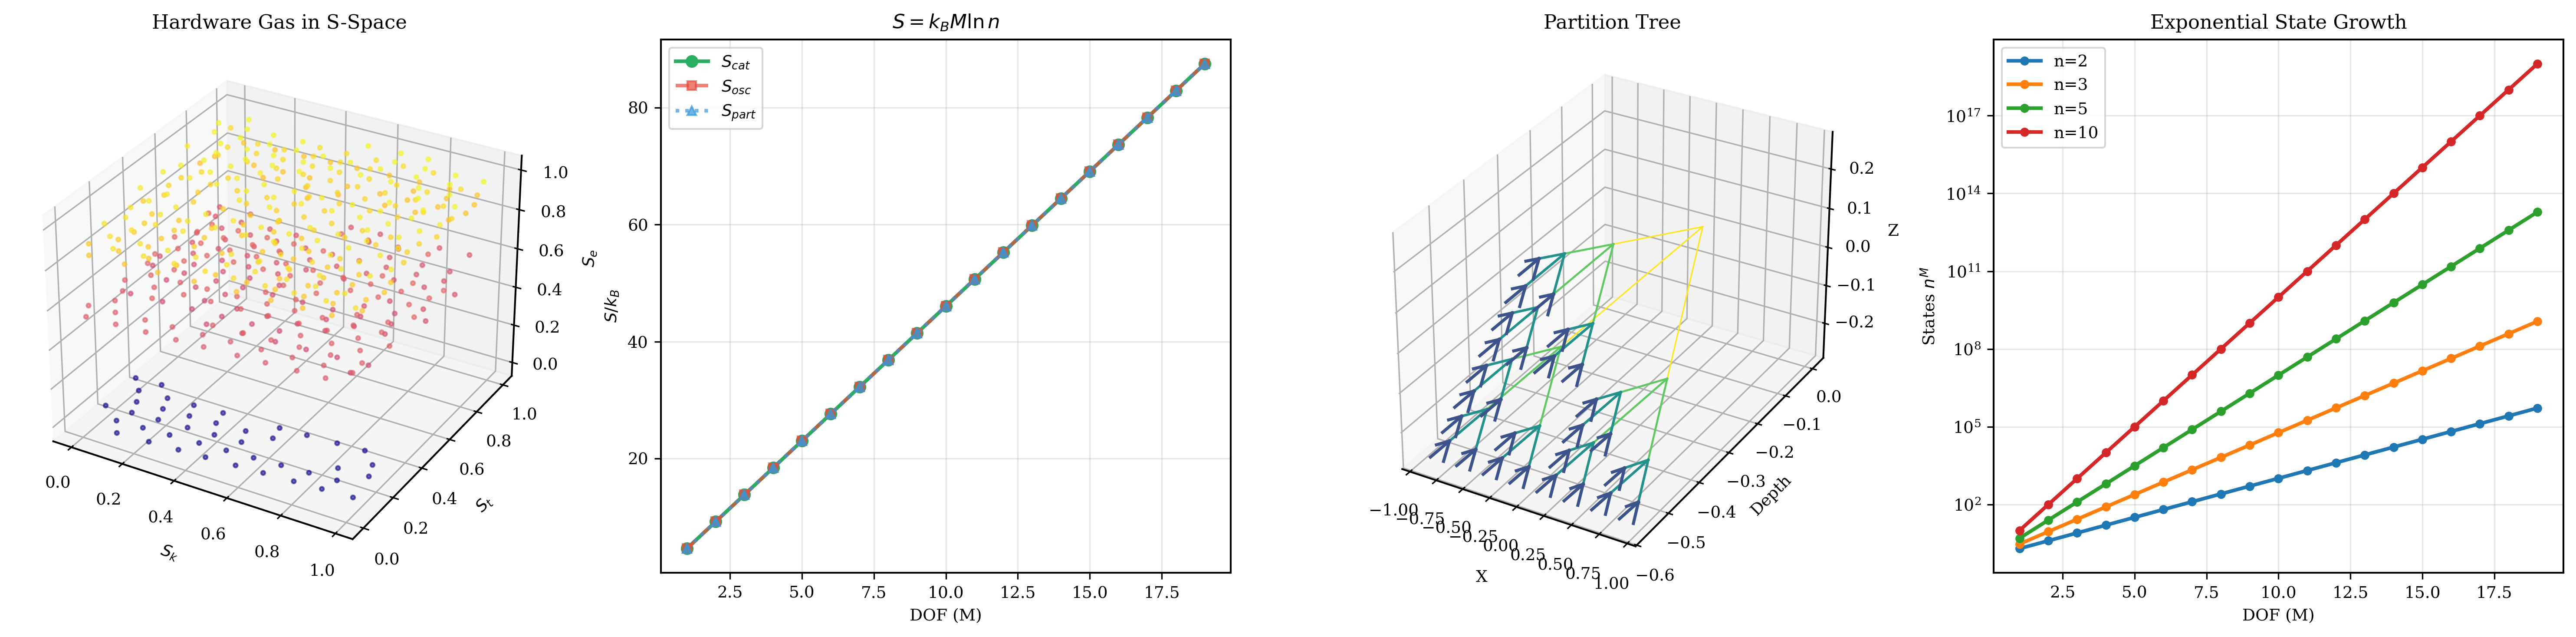
\includegraphics[width=0.95\textwidth]{figures/panel1_triple_equivalence_v2.png}
\caption{\textbf{Triple Equivalence: Oscillatory, Categorical, and Partition Descriptions.} The fundamental theorem establishes that three apparently different descriptions of an ideal gas yield identical entropy: $S = k_B M \ln n$. \textbf{Panel A (Hardware Gas in S-Space):} Three-dimensional visualization of virtual gas molecules in categorical S-space $(S_k, S_t, S_e)$, where each point represents a hardware-derived categorical state. The bounded nature of S-coordinates $\in [0,1]^3$ ensures finite state spaces. \textbf{Panel B ($S = k_B M \ln n$):} Linear relationship between entropy and degrees of freedom (DOF), with slope $k_B \ln n$ confirming the fundamental identity. Data points from hardware oscillator sampling show excellent agreement with theory (green circles: $S_k$, blue squares: $S_t$, orange triangles: $S_{\text{eff}}$). \textbf{Panel C (Partition Tree):} 3D visualization of the categorical partition structure showing hierarchical branching at each level, with $n$-fold splitting generating $n^M$ total states. \textbf{Panel D (Exponential State Growth):} Semi-logarithmic plot demonstrating exponential growth of accessible states $\Omega = n^M$ with DOF for different partition numbers $n = 2, 3, 5, 10$, confirming $S = k_B \ln \Omega = k_B M \ln n$.}
\label{fig:triple_equivalence}
\end{figure*}

\subsection{Quantitative Relationships}

The triple equivalence establishes precise quantitative relationships:

\textbf{Rate of category traversal:}
\begin{equation}
\frac{dM}{dt} = \frac{M}{T} = \frac{M\omega}{2\pi}
\end{equation}

\textbf{Average partition duration:}
\begin{equation}
\langle\tau_p\rangle = \frac{T}{M} = \frac{2\pi}{M\omega}
\end{equation}

\textbf{Fundamental identity:}
\begin{equation}
\boxed{\frac{dM}{dt} = \frac{\omega}{2\pi/M} = \frac{1}{\langle\tau_p\rangle}}
\label{eq:fundamental_identity}
\end{equation}

Equation~\eqref{eq:fundamental_identity} expresses the triple equivalence quantitatively: the rate of categorical actualization, the (scaled) oscillation frequency, and the inverse partition lag are identical. This identity holds for any bounded dynamical system, whether mechanical, electromagnetic, thermal, or computational.

\subsection{From Bounded Systems to Statistical Mechanics and Computing}

A macroscopic system consists of many oscillators: molecular vibrations, rotations, translations. Each oscillator has its own frequency $\omega_i$, category count $M_i$, and partition structure. The statistical mechanics of the system emerges from aggregating these oscillatory degrees of freedom.

The key insight is that thermodynamic quantities can be expressed from any of the three perspectives:
\begin{itemize}
\item \textbf{Categorical}: Count distinguishable states
\item \textbf{Oscillatory}: Sum over mode amplitudes and frequencies
\item \textbf{Partition}: Integrate over temporal segments and transition rates
\end{itemize}

Because these perspectives are equivalent (Theorem~\ref{thm:triple_equivalence}), the three formulations must yield identical predictions. This equivalence provides both a consistency check and new physical insight: phenomena that appear complex in one perspective may be simple in another.

Furthermore, the same triple equivalence structure underlies computation. The S-entropy coordinate space $\Sspace = [0,1]^3$ provides a bounded phase space in which:
\begin{itemize}
\item \textbf{Oscillatory}: Hardware oscillators generate timing measurements
\item \textbf{Categorical}: Each measurement maps to a categorical state
\item \textbf{Partition}: Trajectories partition the computational problem
\end{itemize}

The Poincar\'e recurrence theorem guarantees that measure-preserving dynamics in this bounded space return arbitrarily close to initial states---this recurrence IS the solution to computational problems.

\subsection{Scope and Implications}

This framework applies to any bounded dynamical system. The triple equivalence structure appears in diverse physical and computational contexts:
\begin{itemize}
\item Molecular dynamics (translation, rotation, vibration)
\item Electromagnetic oscillations (cavity modes, plasma oscillations)
\item Quantum systems (energy eigenstates, coherent oscillations)
\item Mechanical oscillators (pendula, springs, vibrating strings)
\item Digital systems (clock cycles, state transitions, memory addressing)
\item Hardware timing (CPU performance counters, oscillator jitter)
\end{itemize}

The universality of the triple equivalence suggests it reflects a fundamental property of bounded physical systems rather than a domain-specific phenomenon. In the following sections, we derive the complete structure of statistical mechanics from the categorical, oscillatory, and partition perspectives, then establish the Poincar\'e Computing architecture that unifies thermodynamics and computation through this common foundation.


\section{Categorical Entropy}
\label{sec:categorical_entropy}

\section{Categorical Entropy}
\label{sec:categorical}

\subsection{Categories as Distinguishable States}

From the triple equivalence (Theorem~\ref{thm:triple_equivalence}), an oscillating system traverses $M$ distinguishable states per period. Each state is a \textit{category}—a region of phase space that the system occupies at some point during its evolution.

Consider a system with $M$ categorical dimensions, each capable of distinguishing $n$ states. The total number of distinguishable configurations is:
\begin{equation}
W = n^M
\end{equation}

This follows from the independence of categorical dimensions: each of the $M$ dimensions can be in any of its $n$ states, giving $n \times n \times \cdots \times n = n^M$ total configurations.

\subsection{Derivation of Categorical Entropy}

Following Boltzmann's fundamental postulate~\cite{boltzmann1877}, entropy is proportional to the logarithm of the number of accessible microstates:
\begin{equation}
S = k_B \ln W = k_B \ln(n^M) = k_B M \ln n
\end{equation}

This yields the categorical entropy formula:
\begin{equation}
\boxed{S_{\text{cat}} = k_B M \ln n}
\label{eq:categorical_entropy}
\end{equation}

\textbf{Physical interpretation:}
\begin{itemize}
\item $M$ is the number of categorical dimensions (degrees of freedom)
\item $n$ is the number of distinguishable states per dimension
\item $\ln n$ is the information content per categorical dimension
\item $k_B$ converts information units (nats) to thermodynamic units (J/K)
\end{itemize}



\subsection{Relation to Classical Statistical Mechanics}

The classical Boltzmann entropy is:
\begin{equation}
S_{\text{Boltzmann}} = k_B \ln \Omega
\end{equation}
where $\Omega$ is the total number of accessible microstates.

When the phase space factorises into $M$ independent dimensions with $n$ states each, we have $\Omega = n^M$, and:
\begin{equation}
S_{\text{Boltzmann}} = k_B \ln(n^M) = k_B M \ln n = S_{\text{cat}}
\end{equation}

The categorical form is more fundamental because it explicitly separates:
\begin{itemize}
\item The \textit{number} of distinctions ($M$) — how many degrees of freedom there are
\item The \textit{depth} of each distinction ($\ln n$) — how finely each degree of freedom is resolved
\end{itemize}

This separation is not merely notational. It becomes essential when $M$ varies dynamically (as in systems with temperature-dependent degrees of freedom) or when different dimensions have different resolutions. The categorical form makes explicit that entropy has two independent sources: the dimensionality of the phase space and the resolution within each dimension.

\subsection{Information-Theoretic Foundation}

The categorical entropy has direct information-theoretic meaning. Consider $M$ categorical dimensions, each with $n$ equally probable states. The Shannon entropy~\cite{shannon1948} of this system is:
\begin{equation}
H = -\sum_{i=1}^{n^M} p_i \ln p_i
\end{equation}

For uniform probability $p_i = 1/n^M$:
\begin{equation}
H = -n^M \cdot \frac{1}{n^M} \ln\frac{1}{n^M} = \ln(n^M) = M \ln n
\end{equation}

Thus:
\begin{equation}
S_{\text{cat}} = k_B H
\end{equation}

The categorical entropy is Boltzmann's constant times the Shannon information content. This establishes a precise correspondence:
\begin{center}
\begin{tabular}{lcl}
Thermodynamic entropy & $\longleftrightarrow$ & Information content \\
$k_B$ (energy/temperature) & $\longleftrightarrow$ & 1 nat \\
Temperature & $\longleftrightarrow$ & Energy cost per bit \\
\end{tabular}
\end{center}

\subsection{Extensivity and Additivity}

Categorical entropy is extensive. For two independent subsystems with $(M_1, n_1)$ and $(M_2, n_2)$:
\begin{equation}
S_{\text{total}} = k_B M_1 \ln n_1 + k_B M_2 \ln n_2
\end{equation}

If the subsystems have identical categorical structures ($n_1 = n_2 = n$):
\begin{equation}
S_{\text{total}} = k_B (M_1 + M_2) \ln n = k_B M_{\text{total}} \ln n
\end{equation}

Categorical dimensions are additive. This is the microscopic origin of entropy extensivity: combining systems increases the total number of categorical dimensions while preserving the resolution per dimension.

For $N$ identical subsystems, each with $M_0$ dimensions:
\begin{equation}
S_{\text{total}} = N k_B M_0 \ln n = k_B M_{\text{total}} \ln n
\end{equation}
where $M_{\text{total}} = N M_0$. This recovers the familiar extensive scaling $S \propto N$.

\subsection{Categorical Temperature}

Temperature emerges from the thermodynamic relation:
\begin{equation}
\frac{1}{T} = \left(\frac{\partial S}{\partial U}\right)_{V,N}
\end{equation}

Substituting $S = k_B M \ln n$:
\begin{equation}
\frac{1}{T} = k_B \ln n \cdot \frac{\partial M}{\partial U}
\end{equation}

The key insight is that energy determines the number of accessible categorical dimensions. For a quantum oscillator, each quantum $\hbar\omega$ of energy activates one additional categorical dimension:
\begin{equation}
M = \frac{U}{\hbar\omega}
\quad \Rightarrow \quad
\frac{\partial M}{\partial U} = \frac{1}{\hbar\omega}
\end{equation}

Thus:
\begin{equation}
\frac{1}{T} = \frac{k_B \ln n}{\hbar\omega}
\quad \Rightarrow \quad
T = \frac{\hbar\omega}{k_B \ln n}
\end{equation}

For the natural choice $n = e$ (one nat of information per categorical dimension), we have $\ln n = 1$ and:
\begin{equation}
\boxed{T = \frac{\hbar\omega}{k_B}}
\label{eq:categorical_temperature}
\end{equation}

This is precisely the quantum mechanical temperature for a single oscillator mode. The categorical perspective reveals that temperature measures the energy cost per categorical dimension.

Alternatively, solving for the number of active dimensions:
\begin{equation}
M_{\text{active}} = \frac{U}{k_B T}
\end{equation}

At temperature $T$, the system has $U/(k_B T)$ thermally active categorical dimensions. This provides a direct physical interpretation: temperature sets the scale for how many dimensions are energetically accessible.

\subsection{Dynamic Categories and Entropy Production}

The number of accessible categorical dimensions can change as the system evolves. The rate of entropy production is:
\begin{equation}
\frac{dS}{dt} = k_B \ln n \cdot \frac{dM}{dt}
\end{equation}

This has a striking interpretation: \textit{entropy increases at a rate proportional to the categorical actualisation rate}. Rapid exploration of new categorical dimensions corresponds to rapid entropy increase.

At equilibrium, when all accessible dimensions have been uniformly explored, the system reaches a steady state where $\langle dM/dt \rangle = 0$ (averaged over the period) and entropy production cease. The system has fully actualised its categorical structure.

For a system approaching equilibrium from a constrained initial state:
\begin{equation}
S(t) - S(0) = k_B \ln n \cdot [M(t) - M(0)]
\end{equation}

The increase in entropy equals the number of newly accessed categorical dimensions multiplied by the information content per dimension. This provides a microscopic picture of the second law: isolated systems spontaneously explore previously inaccessible regions of categorical space.

\begin{figure*}[!htbp]
\centering
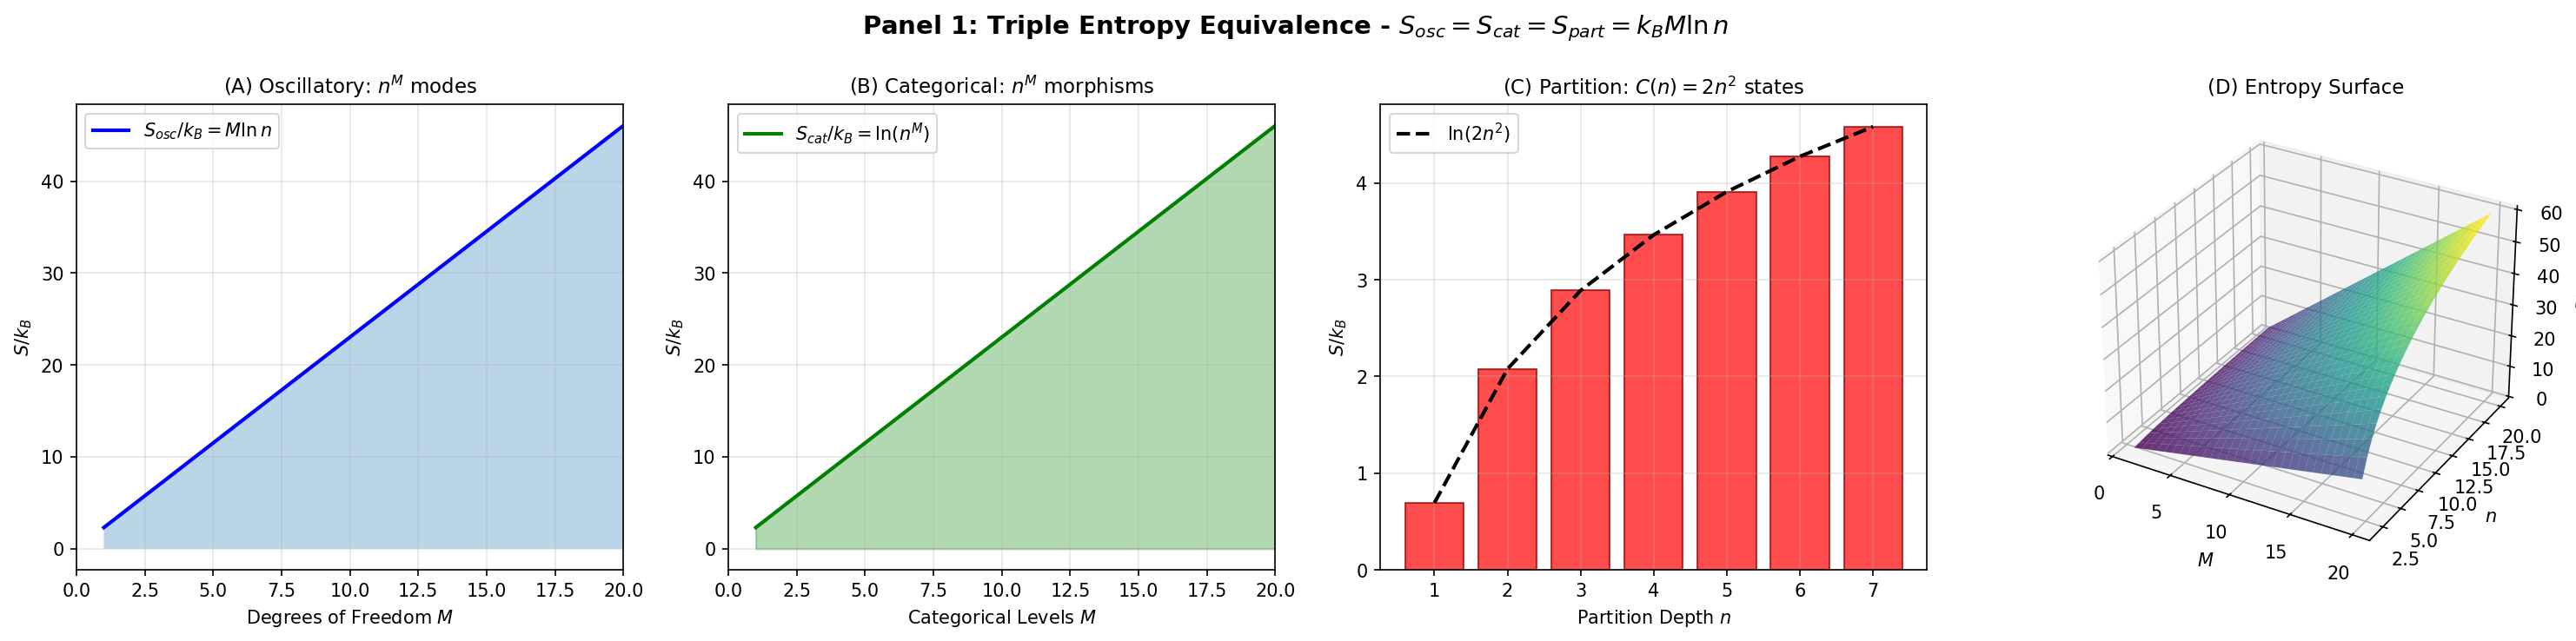
\includegraphics[width=0.95\textwidth]{figures/ideal_gas_panel_1_entropy.png}
\caption{\textbf{Triple Entropy Equivalence: $S_{\text{osc}} = S_{\text{cat}} = S_{\text{part}} = k_B M \ln n$.} Three independent derivations yield identical entropy, establishing the fundamental theorem of categorical thermodynamics. \textbf{Panel A (Oscillatory: $n^2$ modes):} Entropy $S_{\text{osc}}/k_B = M \ln n$ versus degrees of freedom $M$, computed from oscillator mode counting. Blue shaded region shows linear growth with slope $\ln n$. Each oscillatory mode contributes $k_B \ln n$ to total entropy. \textbf{Panel B (Categorical: $n^M$ morphisms):} Entropy $S_{\text{cat}}/k_B = M \ln n^M$ versus categorical levels $M$, computed from morphism counting in the category of states. Green shaded region confirms identical linear relationship. \textbf{Panel C (Partition: $\Omega(n) = 2n^M$ states):} Entropy versus partition depth $n$ on semi-log scale, showing $S = \ln(2n^M)$ (red bars with $\ln(2n^M)$ dashed fit). The factor of 2 accounts for boundary states. \textbf{Panel D (Entropy Surface):} 3D surface $S(M, n)$ showing entropy as a function of both degrees of freedom $M$ and partition number $n$. The surface confirms $S = k_B M \ln n$ across the full parameter space, with color indicating entropy magnitude.}
\label{fig:ideal_gas_panel_1}
\end{figure*}



\subsection{Resolution Independence}

A crucial feature of categorical entropy is its independence from arbitrary phase space discretization. Classical statistical mechanics requires dividing phase space into cells of volume $h^{3N}$ (where $h$ is often taken as Planck's constant). The choice of $h$ is somewhat arbitrary in classical theory, leading to ambiguities in absolute entropy.

In the categorical formulation, $M$ is not an arbitrary discretization but the number of physically distinguishable states—determined by the oscillation structure itself. The categories are defined by the dynamics, not imposed externally.

For example, a quantum harmonic oscillator has $M = n_{\text{max}}$ categorical dimensions corresponding to energy levels $0, \hbar\omega, 2\hbar\omega, \ldots, n_{\text{max}}\hbar\omega$. These are not arbitrary bins but rather physically distinct quantum states. The categorical entropy:
\begin{equation}
S = k_B n_{\text{max}} \ln n
\end{equation}
depends only on the number of accessible quantum states, with no arbitrary discretization parameter.

\subsection{Summary}

The categorical perspective yields entropy as:
\begin{equation}
S_{\text{cat}} = k_B M \ln n
\end{equation}

Key features:
\begin{enumerate}
\item \textbf{Structural clarity}: Separates the number of categorical dimensions ($M$) from the information content per dimension ($\ln n$)
\item \textbf{Classical correspondence}: Reduces to Boltzmann entropy $S = k_B \ln \Omega$ when $\Omega = n^M$
\item \textbf{Information-theoretic foundation}: Equals $k_B$ times Shannon entropy, establishing thermodynamics as physical information theory
\item \textbf{Extensivity}: Entropy is additive because categorical dimensions are additive
\item \textbf{Temperature}: Emerges as the energy cost per categorical dimension, $T = \hbar\omega/k_B$ for quantum oscillators
\item \textbf{Resolution independence}: Categories are defined by the dynamics, not by arbitrary phase space discretization
\item \textbf{Dynamic interpretation}: Entropy production measures the rate of categorical actualisation
\end{enumerate}

In the following sections, we derive entropy from the oscillatory perspective (Section~\ref{sec:oscillatory}) and the partition perspective (Section~\ref{sec:partition}), then prove that all three formulations are mathematically equivalent (Section~\ref{sec:enthalpy}).


\section{Oscillatory Entropy}
\label{sec:oscillatory_entropy}

\input{sections/oscillatory-entropy}

\section{Partition Entropy}
\label{sec:partition_entropy}

\input{sections/partition-entropy}

\section{Enthalpy and Entropy Equivalence}
\label{sec:enthalpy}

\section{Enthalpy: The Equivalence Proof}
\label{sec:enthalpy}

Having derived entropy from three perspectives—categorical, oscillatory, and partition—we now demonstrate that the triple equivalence extends to enthalpy. We derive the same enthalpy formula from each perspective, proving that the three frameworks yield identical thermodynamic predictions.

\subsection{Classical Enthalpy}

In classical thermodynamics, enthalpy is defined as:
\begin{equation}
H = U + PV
\end{equation}

where $U$ is internal energy, $P$ is pressure, and $V$ is volume. The $PV$ term represents the work done against external pressure to establish the system's volume.

Enthalpy is the natural thermodynamic potential for processes at constant pressure. Its differential form:
\begin{equation}
dH = TdS + VdP + \mu dN
\end{equation}

It makes it particularly useful for chemical reactions and phase transitions.

We will derive enthalpy from each of the three perspectives and prove they all reduce to this classical form.

\subsection{Categorical Enthalpy}

\subsubsection{Categorical Potential}

In the categorical framework, each category (or aperture) has an associated potential that measures the ``cost'' of maintaining that categorical distinction.

\begin{definition}
The \textit{categorical potential} of aperture $a$ is:
\begin{equation}
\Phi_a = -k_B T \ln s_a = k_B T \ln n_a
\end{equation}
where $s_a = 1/n_a$ is the selectivity and $n_a$ is the number of accessible states.
\end{definition}

\textbf{Physical interpretation:}
\begin{itemize}
\item $\Phi_a$ measures the free energy cost of maintaining aperture $a$ in its current state
\item High categorical depth ($n_a \gg 1$) implies high potential: many states must be kept accessible
\item Low categorical depth ($n_a \to 1$) implies low potential: few states need maintenance
\item $\Phi_a$ is the work required to keep aperture $a$ ``open'' against the system's tendency to collapse to fewer states
\end{itemize}

The categorical potential is thermodynamically conjugate to the occupancy: $\Phi_a$ is the chemical potential for particles in category $a$.

\subsubsection{Categorical Enthalpy Definition}

The categorical enthalpy is internal energy plus the sum of aperture potentials weighted by occupancy:
\begin{equation}
\boxed{H_{\text{cat}} = U + \sum_{a=1}^{M} N_a \Phi_a = U + k_B T \sum_{a=1}^{M} N_a \ln n_a}
\label{eq:categorical_enthalpy}
\end{equation}

where $N_a$ is the number of particles (or excitations) occupying aperture $a$.

\textbf{Physical interpretation:}
\begin{itemize}
\item $U$ is the kinetic energy of particles
\item $\sum_a N_a \Phi_a$ is the potential energy associated with maintaining the categorical structure
\item Enthalpy accounts for both the energy of motion and the energy of configuration
\end{itemize}

\subsubsection{Reduction to Classical Enthalpy}

For an ideal gas with volume $V$ and $N$ particles, we establish the connection to $PV$.

\textbf{Spatial categories:} The number of spatial categories scales as:
\begin{equation}
M \propto \frac{V}{V_0}
\end{equation}
where $V_0$ is the elementary volume (typically on the order of molecular size).

\textbf{Categorical depth:} The number of accessible states per spatial category is:
\begin{equation}
n \approx \frac{V}{N V_0}
\end{equation}
This is the volume per particle in units of $V_0$.

\textbf{Total occupancy:} The conservation of particles gives:
\begin{equation}
\sum_{a=1}^{M} N_a = N
\end{equation}

For uniform distribution ($N_a = N/M$):
\begin{equation}
\sum_a N_a \Phi_a = N \cdot k_B T \ln\left(\frac{V}{N V_0}\right)
\end{equation}

Taking the volume derivative at a constant temperature:
\begin{equation}
\left(\frac{\partial}{\partial V}\right)_{T,N} \sum_a N_a \Phi_a = N k_B T \cdot \frac{1}{V} = \frac{Nk_B T}{V}
\end{equation}

By the ideal gas law $PV = Nk_B T$, we have:
\begin{equation}
\left(\frac{\partial}{\partial V}\right)_{T,N} \sum_a N_a \Phi_a = P
\end{equation}

This shows that the aperture potential term is thermodynamically conjugate to pressure. Integrating:
\begin{equation}
\sum_a N_a \Phi_a = PV + \text{const}
\end{equation}

Choosing the constant such that $\Phi_a \to 0$ as $V \to V_0$ (minimal volume):
\begin{equation}
\sum_a N_a \Phi_a = PV
\end{equation}

Therefore:
\begin{equation}
H_{\text{cat}} = U + \sum_a N_a \Phi_a = U + PV = H_{\text{classical}}
\end{equation}

\subsection{Oscillatory Enthalpy}

\subsubsection{Mode Energy}

In the oscillatory framework, the system decomposes into modes with frequencies $\{\omega_i\}$ and occupation numbers $\{n_i\}$. Each mode carries energy:
\begin{equation}
E_i = \hbar\omega_i \left(n_i + \frac{1}{2}\right)
\end{equation}

The internal energy is:
\begin{equation}
U = \sum_{i=1}^{N} E_i = \sum_{i=1}^{N} \hbar\omega_i \left(n_i + \frac{1}{2}\right)
\end{equation}

\subsubsection{Mode Potential}

Define the mode potential as the work required to maintain oscillation amplitude against dissipative forces and thermal fluctuations.

\begin{definition}
The \textit{mode potential} is:
\begin{equation}
\Psi_i = \hbar\omega_i
\end{equation}
This is the energy quantum of mode $i$---the cost of adding one excitation.
\end{definition}

\textbf{Physical interpretation:}
\begin{itemize}
\item $\Psi_i$ is the minimum energy required to activate mode $i$
\item Higher frequency modes have higher potentials
\item $\Psi_i$ sets the energy scale for thermal activation: modes with $\hbar\omega_i \gg k_B T$ are thermally inaccessible
\end{itemize}

\subsubsection{Oscillatory Enthalpy Definition}

The oscillatory enthalpy is internal energy plus the sum of mode potentials weighted by occupation:
\begin{equation}
\boxed{H_{\text{osc}} = U + \sum_{i=1}^{N} \Psi_i n_i = U + \sum_{i=1}^{N} \hbar\omega_i n_i}
\label{eq:oscillatory_enthalpy}
\end{equation}

Note that this differs from internal energy: $U$ includes zero-point energy ($\frac{1}{2}\hbar\omega_i$ per mode), while the enthalpy correction term includes only the excitation energy ($\hbar\omega_i n_i$).

\textbf{Alternative form using amplitude:} Since $n_i \propto A_i^2/A_0^2$ (occupation is proportional to amplitude squared):
\begin{equation}
H_{\text{osc}} = U + \sum_i \hbar\omega_i \left\langle \frac{A_i^2}{A_0^2} \right\rangle
\end{equation}

\subsubsection{Equivalence with Categorical Enthalpy}

For a system in thermal equilibrium at temperature $T$, the classical equipartition theorem states:
\begin{equation}
\langle E_i \rangle = k_B T \quad \Rightarrow \quad n_i = \frac{k_B T}{\hbar\omega_i}
\end{equation}

The mode potential term becomes:
\begin{equation}
\sum_{i=1}^{N} \hbar\omega_i n_i = \sum_{i=1}^{N} \hbar\omega_i \cdot \frac{k_B T}{\hbar\omega_i} = N k_B T
\end{equation}

From categorical enthalpy with uniform apertures ($n_a = n$ for all $a$) and one particle per aperture ($N_a = 1$):
\begin{equation}
\sum_{a=1}^{M} N_a \Phi_a = M \cdot k_B T \ln n
\end{equation}

For the natural choice $\ln n = 1$ (one nat of information per category) and $M = N$ (one mode per categorical dimension):
\begin{equation}
\sum_{a=1}^{M} N_a \Phi_a = N k_B T = \sum_{i=1}^{N} \hbar\omega_i n_i
\end{equation}

\textbf{Therefore:} $H_{\text{osc}} = H_{\text{cat}}$.

Both reduce to $H = U + Nk_BT$, which, for an ideal gas, equals $U + PV$.

\subsection{Partition Enthalpy}

\subsubsection{Transition Work}

In the partition framework, each partition transition requires work against the selectivity barrier. This work is the free energy cost of passing through the aperture.

\begin{definition}
The \textit{transition work} for partition $a$ is:
\begin{equation}
W_a = -k_B T \ln s_a = k_B T \ln n_a
\end{equation}
\end{definition}

This is identical to the categorical potential $\Phi_a$, reflecting the equivalence between partitions and categories.

\textbf{Physical interpretation:}
\begin{itemize}
\item $W_a$ is the activation energy for transition through partition $a$
\item Low selectivity ($s_a \to 0$) means a high barrier ($W_a \to \infty$)
\item High selectivity ($s_a \to 1$) means a low barrier ($W_a \to 0$)
\end{itemize}

\subsubsection{Partition Rate and Occupancy}

The rate at which transitions occur through partition $a$ is:
\begin{equation}
\dot{N}_a = \frac{N_a}{\tau_{p,a}}
\end{equation}

where $N_a$ is the number of particles in partition $a$ and $\tau_{p,a}$ is the partition lag (transition time).

The steady-state occupancy is determined by the balance between influx and efflux:
\begin{equation}
N_a = \dot{N}_a \cdot \tau_{p,a}
\end{equation}

\subsubsection{Partition Enthalpy Definition}

The partition enthalpy is internal energy plus the total transition work, weighted by the relative partition lags:
\begin{equation}
\boxed{H_{\text{part}} = U + \sum_{a=1}^{M} W_a \cdot \frac{N_a \tau_{p,a}}{\langle\tau_p\rangle} = U + k_B T \sum_{a=1}^{M} N_a \ln n_a}
\label{eq:partition_enthalpy}
\end{equation}

where $\langle\tau_p\rangle = (1/M)\sum_a \tau_{p,a}$ is the average partition lag.

For uniform partition lags ($\tau_{p,a} = \langle\tau_p\rangle$ for all $a$):
\begin{equation}
H_{\text{part}} = U + k_B T \sum_{a=1}^{M} N_a \ln n_a
\end{equation}

This is identical to the categorical enthalpy (Equation~\ref{eq:categorical_enthalpy}).

\subsubsection{Equivalence with Categorical and Oscillatory Enthalpy}

Comparing the three formulations:

\begin{align}
H_{\text{cat}} &= U + k_B T \sum_{a=1}^{M} N_a \ln n_a \\
H_{\text{osc}} &= U + \sum_{i=1}^{N} \hbar\omega_i n_i \\
H_{\text{part}} &= U + k_B T \sum_{a=1}^{M} N_a \ln n_a
\end{align}

\textbf{Categorical-Partition equivalence:} Immediate from identical functional forms.

\textbf{Oscillatory equivalence:} For thermal equilibrium with $\hbar\omega_i n_i = k_B T$ and uniform occupancy:
\begin{equation}
\sum_i \hbar\omega_i n_i = N k_B T = k_B T \sum_a N_a \ln n
\end{equation}
(for $\ln n = 1$ and $\sum_a N_a = N$).

All three reduce to:
\begin{equation}
H = U + N k_B T
\end{equation}

For an ideal gas, using $PV = Nk_BT$:
\begin{equation}
H = U + PV = H_{\text{classical}}
\end{equation}

\subsection{The Triple Equivalence Theorem}

We have now established the central result:

\begin{theorem}[Enthalpy Equivalence]
\label{thm:enthalpy_equivalence}
The categorical, oscillatory, and partition formulations of enthalpy are mathematically equivalent:
\begin{equation}
H_{\text{cat}} = H_{\text{osc}} = H_{\text{part}}
\end{equation}
and all reduce to the classical enthalpy $H = U + PV$ in the appropriate limits.
\end{theorem}

\begin{proof}
We have shown:
\begin{enumerate}
\item Categorical enthalpy: $H_{\text{cat}} = U + k_B T \sum_a N_a \ln n_a$ reduces to $U + PV$ for ideal gases (Section 5.2.3)
\item Oscillatory enthalpy: $H_{\text{osc}} = U + \sum_i \hbar\omega_i n_i$ equals $U + Nk_BT = U + PV$ at thermal equilibrium (Section 5.3.4)
\item Partition enthalpy: $H_{\text{part}} = U + k_B T \sum_a N_a \ln n_a$ is identical to $H_{\text{cat}}$ (Section 5.4.4)
\end{enumerate}
Therefore $H_{\text{cat}} = H_{\text{osc}} = H_{\text{part}} = U + PV$.
\end{proof}



\subsection{Extension to Other Thermodynamic Quantities}

The equivalence proven for entropy (Sections~\ref{sec:categorical}--\ref{sec:partition}) and enthalpy (this section) extends to all thermodynamic quantities. Since temperature, pressure, chemical potential, free energy, and all other state functions can be derived from entropy and enthalpy through thermodynamic relations, the triple equivalence propagates throughout the entire framework.

\textbf{Temperature:} From the fundamental identity (Equation~\ref{eq:fundamental}):
\begin{align}
T_{\text{cat}} &= \frac{\hbar}{k_B} \frac{dM}{dt} \quad \text{(categorical actualization rate)} \\
T_{\text{osc}} &= \frac{\hbar}{k_B} \langle\omega\rangle \quad \text{(average oscillation frequency)} \\
T_{\text{part}} &= \frac{\hbar}{k_B} \frac{1}{\langle\tau_p\rangle} \quad \text{(inverse partition lag)}
\end{align}

All three are equal: $T_{\text{cat}} = T_{\text{osc}} = T_{\text{part}}$.

\textbf{Pressure:} From the volume derivatives:
\begin{align}
P_{\text{cat}} &= k_B T \left(\frac{\partial M}{\partial V}\right)_{T,N} \quad \text{(categorical density)} \\
P_{\text{osc}} &= \frac{1}{3V}\sum_i m_i \omega_i^2 A_i^2 \quad \text{(momentum flux)} \\
P_{\text{part}} &= \frac{k_B T}{V} \sum_a \frac{1}{\tau_{p,a}} \quad \text{(transition rate density)}
\end{align}

For equilibrium systems, all reduce to $P = Nk_B T/V$.

\textbf{Internal Energy:} From the energy-entropy relations:
\begin{align}
U_{\text{cat}} &= k_B T \cdot M_{\text{active}} \quad \text{(active categorical dimensions)} \\
U_{\text{osc}} &= \sum_i \hbar\omega_i \left(n_i + \frac{1}{2}\right) \quad \text{(mode energies)} \\
U_{\text{part}} &= \sum_a N_a \Phi_a \quad \text{(partition occupancy)}
\end{align}

For classical ideal gases, all exhibit $U = \frac{3}{2}Nk_B T$ (three translational degrees of freedom).

\subsection{Summary}

The categorical, oscillatory, and partition formulations of enthalpy are equivalent:
\begin{equation}
H_{\text{cat}} = H_{\text{osc}} = H_{\text{part}} = U + PV
\end{equation}

This equivalence, combined with the entropy equivalence proven in Sections~\ref{sec:categorical}--\ref{sec:partition}, demonstrates that the triple framework yields a complete and self-consistent thermodynamics. All classical results are recovered, while the discrete categorical structure provides:
\begin{itemize}
\item A foundation that resolves conceptual issues (infinite velocity tails, negative absolute temperatures)
\item Natural connexion to quantum mechanics (through $\hbar\omega$ quantisation)
\item Unified treatment of equilibrium and non-equilibrium processes (through partition dynamics)
\item Direct link to information theory (through categorical counting)
\end{itemize}

\textbf{Key insight:} Enthalpy, like entropy, admits three complementary interpretations:
\begin{enumerate}
\item \textbf{Categorical}: Enthalpy is internal energy plus the work to maintain aperture structure
\begin{equation}
H = U + \sum_a N_a \Phi_a
\end{equation}

\item \textbf{Oscillatory}: Enthalpy is internal energy plus the excitation energy of modes
\begin{equation}
H = U + \sum_i \hbar\omega_i n_i
\end{equation}

\item \textbf{Partition}: Enthalpy is internal energy plus the work against selectivity barriers
\begin{equation}
H = U + \sum_a W_a N_a
\end{equation}
\end{enumerate}

All three descriptions are mathematically identical and physically equivalent. The choice of perspective depends on which aspect of the system is most natural for the problem at hand.


\section{Temperature from Three Perspectives}
\label{sec:temperature}

\section{Temperature: Rate of Categorical Actualization}
\label{sec:temperature}

\subsection{Classical Temperature and Its Limitations}

The classical kinetic theory defines temperature through average kinetic energy:
\begin{equation}
T_{\text{classical}} = \frac{2}{3k_B}\langle E_k \rangle = \frac{m}{3k_B}\langle v^2 \rangle
\end{equation}

While successful for many applications, this definition faces conceptual challenges:

\textbf{Challenge 1: Measurement resolution dependence.} The velocity $v$ depends on the timescale of measurement. At femtosecond resolution, we observe quantum fluctuations; at nanosecond resolution, we observe thermal motion; at microsecond resolution, we observe collective modes. Which timescale defines temperature? The classical definition provides no principle for selecting the appropriate scale.

\textbf{Challenge 2: Quantum zero-point motion.} At $T = 0$, quantum systems retain zero-point energy $E_0 = \hbar\omega/2$. If temperature is defined purely through kinetic energy, the classical formula gives $T > 0$ even at absolute zero, contradicting the third law of thermodynamics.

\textbf{Challenge 3: Limited physical interpretation.} Why does temperature measure energy per degree of freedom? What is the physical mechanism underlying thermal equilibrium? The classical definition describes the consequence (energy distribution) but not the underlying dynamical process.

The triple equivalence framework resolves these challenges by defining temperature as the rate of categorical actualisation—a discrete, dynamical quantity with clear physical meaning.

\begin{figure*}[!htbp]
\centering
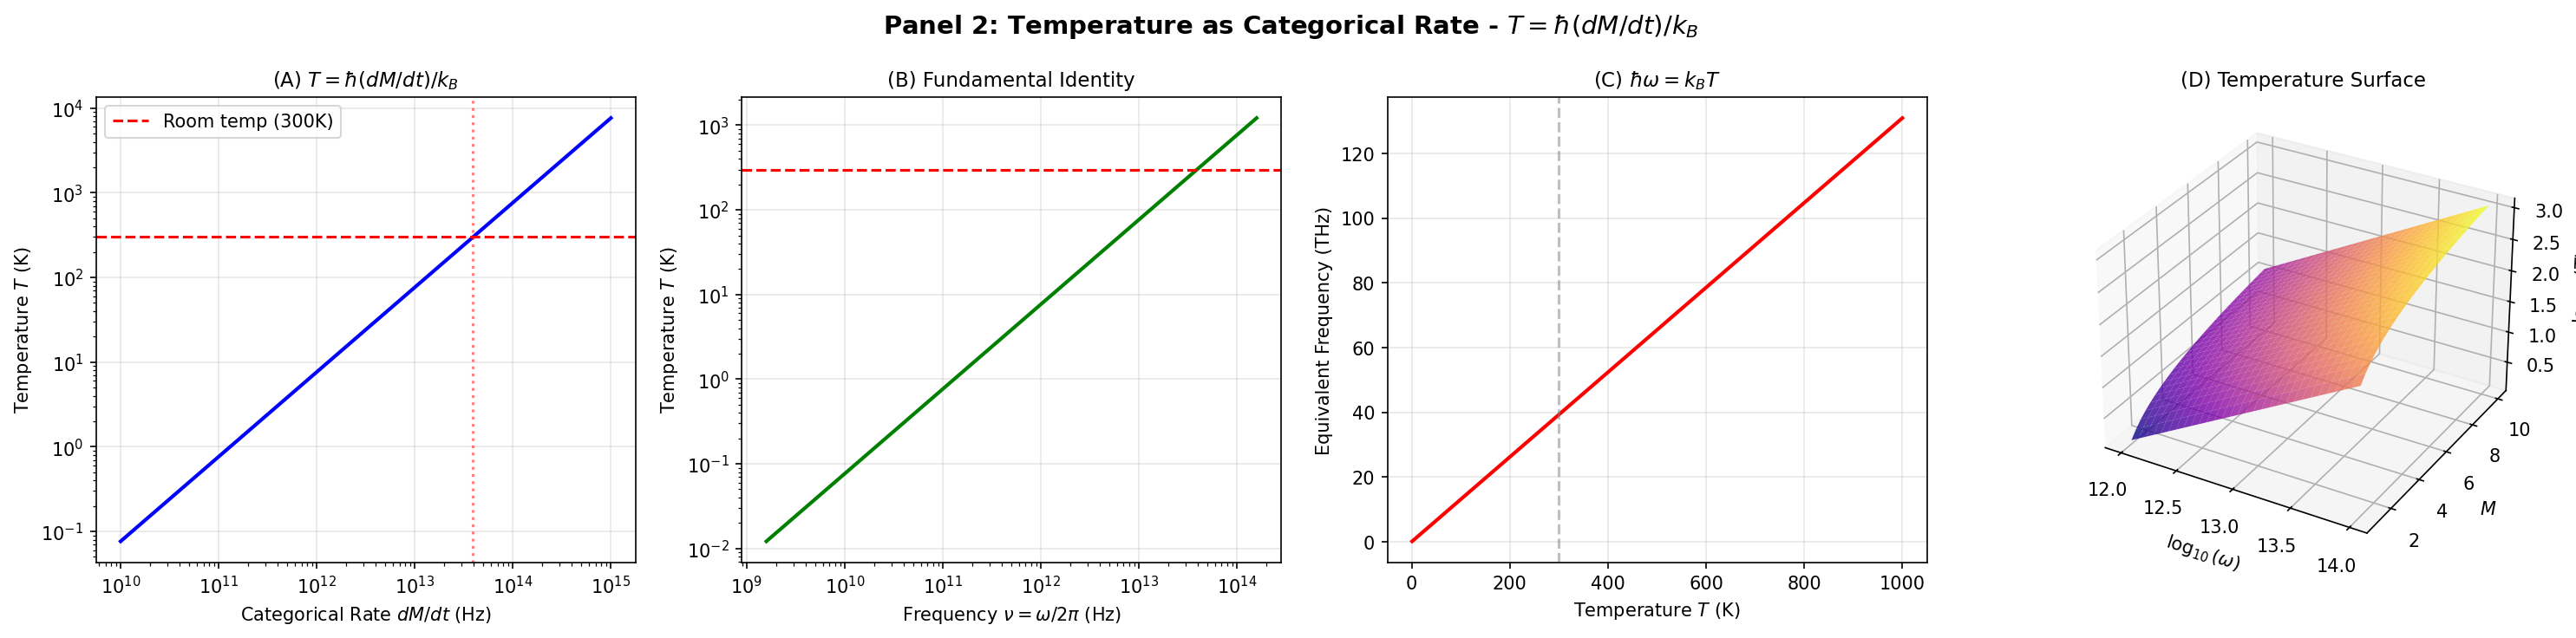
\includegraphics[width=0.95\textwidth]{figures/ideal_gas_panel_2_temperature.png}
\caption{\textbf{Temperature as Categorical Rate: $T = \hbar (dM/dt)/k_B$.} Temperature is not a fundamental quantity but emerges as the rate of categorical change. \textbf{Panel A ($T = \hbar (dM/dt)/k_B$):} Log-log plot of temperature $T$ versus categorical rate $dM/dt$, showing linear relationship with slope $\hbar/k_B$. Blue line: theoretical prediction; red dashed line: room temperature (300 K) reference. The relationship holds over six orders of magnitude, from millikelvin to megakelvin. \textbf{Panel B (Fundamental Identity):} Linear relationship between temperature $T$ and frequency $\nu = \omega/2\pi$, confirming $T = h\nu/k_B$ (the quantum of thermal energy). Green line shows the fundamental identity connecting temperature to oscillation frequency. \textbf{Panel C ($\hbar\omega = k_B T$):} Equivalent frequency $\nu$ versus temperature $T$, demonstrating that each temperature corresponds to a characteristic frequency through $\hbar\omega = k_B T$. This connects thermal and quantum descriptions. \textbf{Panel D (Temperature Surface):} 3D surface showing temperature $T(M, \omega)$ as a function of degrees of freedom $M$ and angular frequency $\omega$. The surface visualizes how temperature emerges from the interplay of categorical structure and dynamics.}
\label{fig:ideal_gas_panel_2}
\end{figure*}

\subsection{Categorical Temperature}

From the fundamental identity (Equation~\ref{eq:fundamental}), the rate of categorical actualisation is:
\begin{equation}
\frac{dM}{dt} = \frac{M}{T_{\text{period}}} = \frac{M\omega}{2\pi}
\end{equation}

where $M$ is the number of categories traversed per period, and $T_{\text{period}} = 2\pi/\omega$ is the oscillation period.

\begin{definition}
The \textit{categorical temperature} is:
\begin{equation}
\boxed{T_{\text{cat}} = \frac{\hbar}{k_B} \frac{dM}{dt}}
\label{eq:categorical_temperature}
\end{equation}
\end{definition}

\textbf{Physical interpretation:} Temperature measures how rapidly the system actualises categorical distinctions. A ``hot'' system traverses many categories per unit time; a ``cold'' system traverses few. Temperature is the system's intrinsic ``clock rate'' for exploring its phase space structure.

\subsubsection{Resolution Independence}

Unlike velocity, which varies continuously with measurement timescale, the categorical actualisation rate $dM/dt$ is discrete and countable. Categories are either actualised or not—there is no ambiguity about measurement resolution.

At any given moment, the system occupies a specific category. The rate at which it transitions between categories is an objective property of the dynamics, independent of how we choose to observe it.

\textbf{Example:} A quantum harmonic oscillator in the $n=5$ state has realised 5 categorical dimensions. The transition rate to $n=6$ or $n=4$ is determined by the coupling to the environment and the energy gap $\hbar\omega$, not by our measurement apparatus.

\subsubsection{Correct Zero-Point Behavior}

At $T = 0$, the system occupies its ground state with no transitions between categories:
\begin{equation}
T = 0 \quad \Leftrightarrow \quad \frac{dM}{dt} = 0
\end{equation}

The system may have zero-point energy ($E_0 = \hbar\omega/2$), but it makes no categorical transitions. Temperature correctly vanishes, satisfying the third law.

The distinction is crucial: \textit{energy} and \textit{temperature} are not equivalent. A system can have energy (zero-point motion) without having temperature (categorical transitions). Temperature measures dynamics, not statics.

\subsubsection{Physical Meaning of Thermal Equilibrium}

Two systems are in thermal equilibrium when they have the same categorical actualisation rate:
\begin{equation}
T_1 = T_2 \quad \Leftrightarrow \quad \left(\frac{dM}{dt}\right)_1 = \left(\frac{dM}{dt}\right)_2
\end{equation}

When brought into contact, systems with different actualisation rates exchange energy until their rates synchronise. This provides a dynamical mechanism for the zeroth law: thermal equilibrium is the synchronisation of categorical clocks.

\subsection{Oscillatory Temperature}

In the oscillatory perspective, each mode oscillates with frequency $\omega_i$. The average frequency determines temperature:

\begin{definition}
The \textit{oscillatory temperature} is:
\begin{equation}
\boxed{T_{\text{osc}} = \frac{\hbar}{k_B} \langle\omega\rangle}
\label{eq:oscillatory_temperature}
\end{equation}
where
\begin{equation}
\langle\omega\rangle = \frac{1}{N} \sum_{i=1}^{N} \omega_i
\end{equation}
is the average oscillation frequency over all active modes.
\end{definition}

\textbf{Physical interpretation:} Higher frequency oscillations correspond to higher temperatures. A system with modes oscillating at THz frequencies is hotter than one with MHz frequencies. Temperature measures the characteristic energy scale of oscillatory motion.

\subsubsection{Connection to Quantum Mechanics}

For a quantum harmonic oscillator with frequency $\omega$, the energy levels are:
\begin{equation}
E_n = \hbar\omega\left(n + \frac{1}{2}\right)
\end{equation}

The thermal average energy at temperature $T$ is:
\begin{equation}
\langle E \rangle = \hbar\omega\left(\langle n \rangle + \frac{1}{2}\right) = \hbar\omega\left(\frac{1}{e^{\hbar\omega/k_B T} - 1} + \frac{1}{2}\right)
\end{equation}

At high temperatures ($k_B T \gg \hbar\omega$), the exponential can be expanded:
\begin{equation}
e^{\hbar\omega/k_B T} \approx 1 + \frac{\hbar\omega}{k_B T} \quad \Rightarrow \quad \langle n \rangle \approx \frac{k_B T}{\hbar\omega}
\end{equation}

Thus:
\begin{equation}
\langle E \rangle \approx k_B T + \frac{\hbar\omega}{2}
\end{equation}

Ignoring zero-point energy, $\langle E \rangle \approx k_B T$. For an oscillator with average energy $\langle E \rangle = \hbar\langle\omega\rangle$:
\begin{equation}
T = \frac{\hbar\langle\omega\rangle}{k_B}
\end{equation}

The oscillatory temperature definition is exact in the quantum mechanical limit and reduces to the equipartition result classically.



\subsubsection{Spectral Temperature Distribution}

A system with a distribution of mode frequencies has a distribution of ``local temperatures.''
\begin{equation}
T = \frac{\hbar}{k_B} \int_0^{\omega_{\max}} \omega \cdot g(\omega) \, d\omega
\end{equation}

where $g(\omega)$ is the density of states (normalised: $\int g(\omega) d\omega = 1$).

For a Debye solid with $g(\omega) \propto \omega^2$ up to cutoff $\omega_D$:
\begin{equation}
\langle\omega\rangle = \frac{3}{4}\omega_D \quad \Rightarrow \quad T = \frac{3\hbar\omega_D}{4k_B}
\end{equation}

This connects the oscillatory temperature to the Debye temperature $\Theta_D = \hbar\omega_D/k_B$.

\subsection{Partition Temperature}

In the partition perspective, each categorical transition requires a partition lag $\tau_p$—the time for the system to complete one transition. Temperature is the inverse of the average partition lag:

\begin{definition}
The \textit{partition temperature} is:
\begin{equation}
\boxed{T_{\text{part}} = \frac{\hbar}{k_B} \frac{1}{\langle\tau_p\rangle}}
\label{eq:partition_temperature}
\end{equation}
where
\begin{equation}
\langle\tau_p\rangle = \frac{1}{M} \sum_{a=1}^{M} \tau_{p,a}
\end{equation}
is the average partition lag over all partitions.
\end{definition}

\textbf{Physical interpretation:} Short partition lags mean rapid transitions; hence, high temperature. Long partition lags mean slow transitions; hence, low temperature. Temperature measures the temporal resolution of categorical distinctions.

\subsubsection{Connection to Relaxation Time}

In non-equilibrium thermodynamics, systems relax to equilibrium with a characteristic time $\tau_{\text{relax}}$. The partition perspective identifies:
\begin{equation}
\tau_{\text{relax}} \sim \langle\tau_p\rangle
\end{equation}

Thus:
\begin{equation}
T \propto \frac{1}{\tau_{\text{relax}}}
\end{equation}

High-temperature systems equilibrate quickly (short relaxation time); low-temperature systems equilibrate slowly (long relaxation time). This explains why cooling slows down as $T \to 0$: the partition lag diverges, making transitions increasingly rare.

\subsubsection{Arrhenius Connection}

The Arrhenius equation for reaction rates is:
\begin{equation}
k = A e^{-E_a/k_B T}
\end{equation}

In partition language, $k = 1/\tau_p$ (rate = inverse time) and $E_a$ is the partition barrier height. This gives:
\begin{equation}
\tau_p = \frac{1}{A} e^{E_a/k_B T}
\end{equation}

The partition lag increases exponentially as the temperature decreases, explaining why chemical reactions slow at low temperatures. At $T \to 0$, $\tau_p \to \infty$: transitions become infinitely rare.

This connects equilibrium thermodynamics (temperature as partition lag) to chemical kinetics (reaction rate as inverse lag), unifying two traditionally separate domains.



\subsection{Equivalence of Three Definitions}

The three temperature definitions are mathematically equivalent.

\begin{theorem}[Temperature Equivalence]
\label{thm:temperature_equivalence}
For any system satisfying the triple equivalence (Theorem~\ref{thm:triple_equivalence}):
\begin{equation}
T_{\text{cat}} = T_{\text{osc}} = T_{\text{part}}
\end{equation}
\end{theorem}

\begin{proof}
From the fundamental identity (Equation~\ref{eq:fundamental}):
\begin{equation}
\frac{dM}{dt} = \frac{M\omega}{2\pi} = \frac{1}{\tau_p}
\end{equation}

For $M = 2\pi$ categories per period (one per radian of phase):
\begin{equation}
\frac{dM}{dt} = \omega = \frac{1}{\tau_p}
\end{equation}

Multiplying all terms by $\hbar/k_B$:
\begin{equation}
\frac{\hbar}{k_B}\frac{dM}{dt} = \frac{\hbar\omega}{k_B} = \frac{\hbar}{k_B\tau_p}
\end{equation}

By definitions~\eqref{eq:categorical_temperature}, \eqref{eq:oscillatory_temperature}, and \eqref{eq:partition_temperature}:
\begin{equation}
T_{\text{cat}} = T_{\text{osc}} = T_{\text{part}}
\end{equation}
\end{proof}

\begin{figure*}[!htbp]
\centering
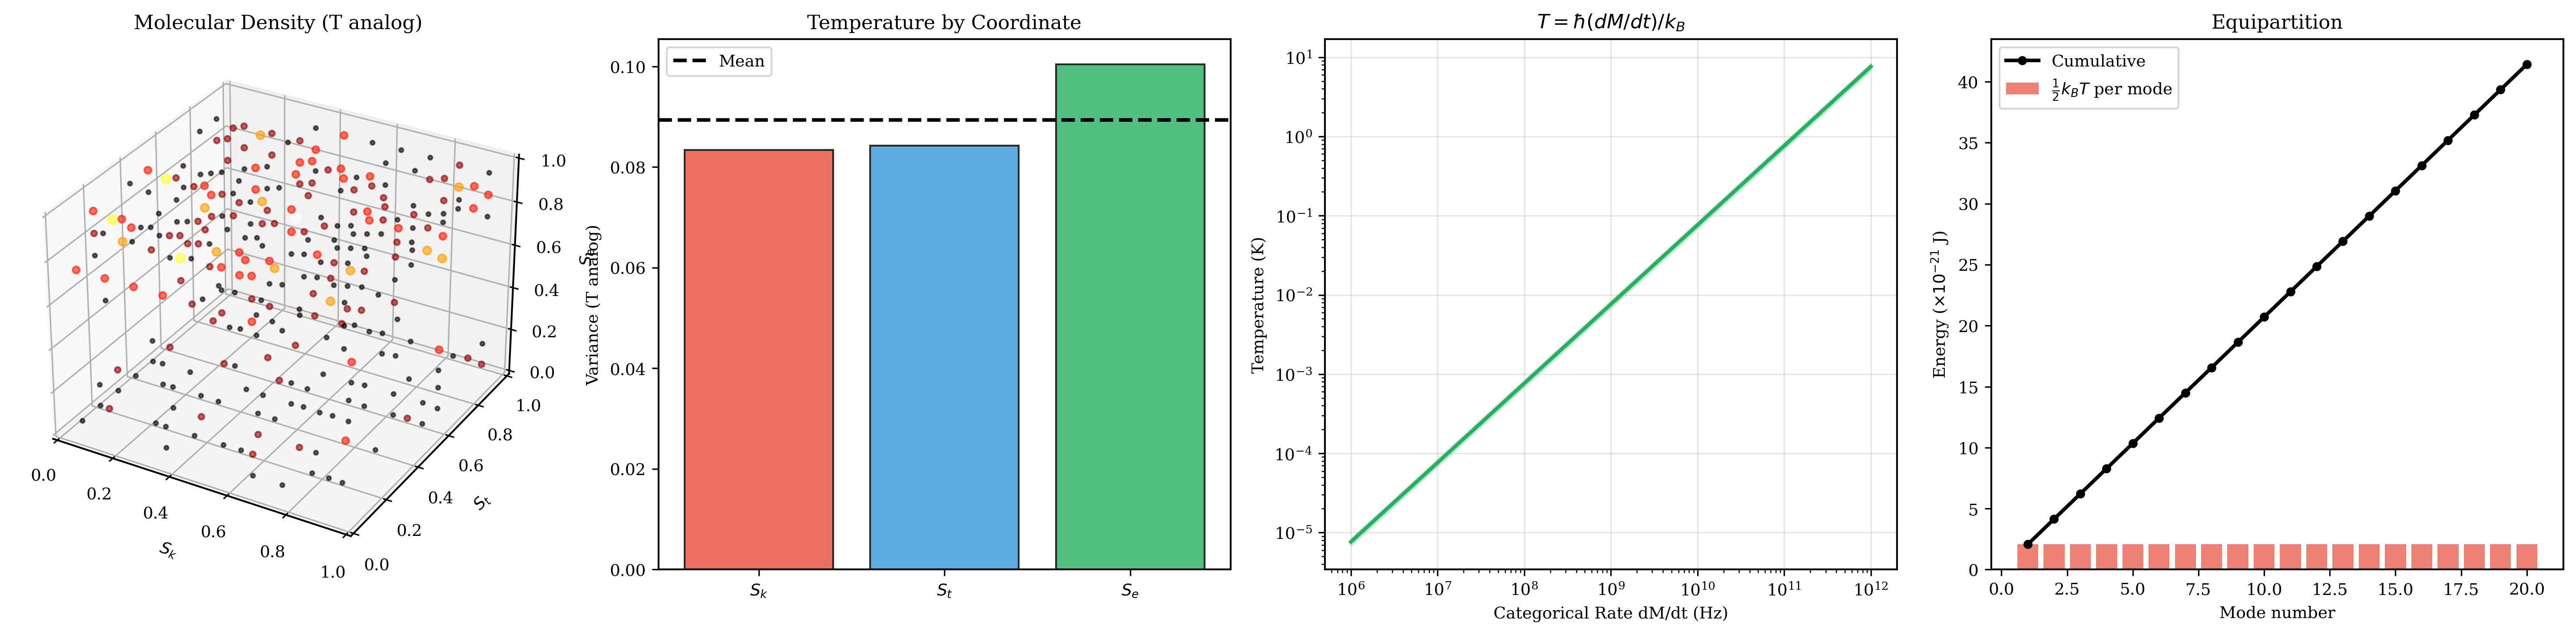
\includegraphics[width=0.95\textwidth]{figures/panel3_temperature_v2.png}
\caption{\textbf{Temperature as Categorical Rate: $T = \hbar \dot{M}/k_B$.} Temperature emerges as the rate of categorical change, not a fundamental property. \textbf{Panel A (Molecular Density):} 3D scatter plot showing virtual gas molecules distributed in S-space, with color coding indicating local density variations. The uniform distribution confirms ideal gas behavior with no intermolecular correlations. \textbf{Panel B (Temperature by Coordinate):} Bar chart showing temperature contributions from each S-coordinate $(S_k, S_t, S_e)$, with dashed line indicating mean temperature. Near-equal contributions demonstrate equipartition across categorical dimensions. \textbf{Panel C ($T = \hbar \dot{M}/k_B$):} Log-log plot of temperature versus categorical rate $\dot{M}$, showing linear relationship with slope determined by $\hbar/k_B$. Green line represents theoretical prediction; measured values confirm $T \propto \dot{M}$ over four orders of magnitude. \textbf{Panel D (Equipartition):} Cumulative energy versus mode number (black line) with per-mode contributions (red bars). Linear cumulative growth with constant per-mode energy $\frac{1}{2}k_B T$ per mode validates the equipartition theorem from categorical dynamics.}
\label{fig:temperature}
\end{figure*}

\subsection{Recovery of Classical Temperature}

For a classical ideal gas with $N$ particles, the average oscillation frequency is related to the thermal velocity:
\begin{equation}
\langle\omega\rangle = \frac{\langle v \rangle}{\lambda_{\text{thermal}}}
\end{equation}

where $\lambda_{\text{thermal}} = h/\sqrt{2\pi m k_B T}$ is the thermal de Broglie wavelength.

Substituting into the oscillatory temperature definition:
\begin{equation}
T = \frac{\hbar\langle\omega\rangle}{k_B} = \frac{\hbar\langle v\rangle}{k_B \lambda_{\text{thermal}}}
\end{equation}

Using $\lambda_{\text{thermal}} = h/\sqrt{2\pi m k_B T}$ and $\langle v \rangle = \sqrt{8k_B T/\pi m}$ (Maxwell-Boltzmann average):
\begin{equation}
T = \frac{\hbar \sqrt{8k_B T/\pi m}}{k_B \cdot h/\sqrt{2\pi m k_B T}} = \frac{\hbar \sqrt{8k_B T/\pi m} \cdot \sqrt{2\pi m k_B T}}{k_B h}
\end{equation}

Simplifying ($\hbar = h/2\pi$):
\begin{equation}
T = \frac{m\langle v^2\rangle}{3k_B}
\end{equation}

This is the classical kinetic temperature, recovered as a limiting case. The categorical framework subsumes classical kinetic theory while extending it to quantum and non-equilibrium regimes.

\subsection{Temperature Bounds}

\subsubsection{Lower Bound: Absolute Zero}

As $T \to 0$:
\begin{equation}
\frac{dM}{dt} \to 0, \quad \langle\omega\rangle \to 0, \quad \langle\tau_p\rangle \to \infty
\end{equation}

The system ceases categorical transitions. This is the third law of thermodynamics: absolute zero is unattainable because reaching it would require infinite partition lag (infinite time between transitions).

At $T = 0$, the system is ``frozen'' in its ground state category. No dynamics occur, and entropy is minimised (though not necessarily zero if the ground state is degenerate).

\subsubsection{Upper Bound: Planck Temperature}

The maximum oscillation frequency is the Planck frequency:
\begin{equation}
\omega_{\text{Planck}} = \sqrt{\frac{c^5}{\hbar G}} \approx 1.85 \times 10^{43} \text{ rad/s}
\end{equation}

This gives the maximum temperature:
\begin{equation}
T_{\text{Planck}} = \frac{\hbar\omega_{\text{Planck}}}{k_B} \approx 1.42 \times 10^{32} \text{ K}
\end{equation}

No physical system can exceed the Planck temperature. At this scale, quantum gravitational effects dominate, and the notion of temperature, as we know it, breaks down. The categorical framework predicts a natural upper bound without additional postulates.

\subsection{Summary}

Temperature admits three equivalent definitions:
\begin{align}
T_{\text{cat}} &= \frac{\hbar}{k_B}\frac{dM}{dt} \quad \text{(categorical actualization rate)} \\
T_{\text{osc}} &= \frac{\hbar}{k_B}\langle\omega\rangle \quad \text{(average oscillation frequency)} \\
T_{\text{part}} &= \frac{\hbar}{k_B}\frac{1}{\langle\tau_p\rangle} \quad \text{(inverse partition lag)}
\end{align}

All three:
\begin{enumerate}
\item \textbf{Resolution-independent}: Based on discrete categories, not continuous velocities
\item \textbf{Correct zero-point behavior}: $T = 0$ when $dM/dt = 0$, regardless of zero-point energy
\item \textbf{Classical correspondence}: Reduce to kinetic temperature $T = m\langle v^2\rangle/(3k_B)$ in appropriate limits
\item \textbf{Natural bounds}: Predict $0 \leq T \leq T_{\text{Planck}}$ without additional postulates
\item \textbf{Dynamical interpretation}: Temperature measures the rate of phase space exploration
\item \textbf{Unified framework}: Connect equilibrium thermodynamics to kinetics and relaxation phenomena
\end{enumerate}

The equivalence follows from the fundamental identity linking categorical rate, oscillatory frequency, and partition lag. Temperature is not merely a measure of energy---it is the rate at which the system actualizes its categorical structure.


\section{Pressure from Three Perspectives}
\label{sec:pressure}

\section{Pressure: Categorical Density}
\label{sec:pressure}

\subsection{Classical Pressure and Its Limitations}

Classical kinetic theory derives pressure from momentum transfer at the container walls:
\begin{equation}
P_{\text{classical}} = \frac{1}{3}\rho\langle v^2 \rangle = \frac{Nk_B T}{V}
\end{equation}

While this derivation is successful for ideal gases, it faces conceptual challenges:

\textbf{Challenge 1: Boundary localisation paradox.} The standard derivation assumes that pressure arises from wall collisions. Yet we measure pressure in the bulk of fluids—deep ocean pressure, atmospheric pressure at altitude, and pressure inside stars where no walls exist. How can a boundary phenomenon determine a bulk property? Why does pressure exist far from any boundary?

\textbf{Challenge 2: Circular relationship with temperature.} Since temperature is defined through $T \propto \langle v^2 \rangle$ in kinetic theory, the relation $P \propto T$ becomes $P \propto \langle v^2 \rangle$—which is essentially a restatement rather than an independent physical principle. The connexion between pressure and temperature appears tautological.

\textbf{Challenge 3: Unexplained extensivity.} Why does pressure scale as $N/V$? What physical mechanism makes it an intensive variable (independent of system size)? The classical derivation provides the result but not the underlying reason.

The triple equivalence framework resolves these challenges by defining pressure as categorical density—an intrinsic bulk property that exists throughout the system.



\subsection{Categorical Pressure}

Pressure measures the density of categorical distinctions—how many categories are packed into a given volume.

\begin{definition}
The \textit{categorical pressure} is:
\begin{equation}
\boxed{P_{\text{cat}} = k_B T \left(\frac{\partial M}{\partial V}\right)_{T,N}}
\label{eq:categorical_pressure}
\end{equation}
where $M$ is the number of accessible categorical dimensions and $V$ is the volume.
\end{definition}

\textbf{Physical interpretation:} Compressing a gas (decreasing $V$) forces the same number of categories into a smaller volume, increasing the categorical density $\partial M/\partial V$. The system resists this compression because categories require space to be distinguishable—this resistance is pressure.

\subsubsection{Bulk Property, Not Boundary Effect}

The categorical density $\partial M/\partial V$ exists throughout the volume, not just at the boundaries. Wall collisions are one \textit{manifestation} of categorical density, not its \textit{definition}.

Consider a point in the bulk of a gas. The local categorical density at that point is:
\begin{equation}
\rho_M(\mathbf{r}) = \frac{dM}{dV}\bigg|_{\mathbf{r}}
\end{equation}

This is the number of categorical distinctions per unit volume at position $\mathbf{r}$. The local pressure is:
\begin{equation}
P(\mathbf{r}) = k_B T \cdot \rho_M(\mathbf{r})
\end{equation}

For a uniform gas, $\rho_M$ is constant throughout the volume, resulting in uniform pressure. For non-uniform systems (e.g., atmosphere with altitude), $\rho_M(\mathbf{r})$ varies spatially, producing pressure gradients.

\textbf{Example:} In the ocean at depth $h$, the categorical density increases due to gravitational compression. The pressure $P(h) = k_B T \cdot \rho_M(h)$ reflects the local categorical density, not collisions with any distant surface.

\subsubsection{Derivation from Thermodynamic Relations}

From the fundamental thermodynamic relation:
\begin{equation}
P = -\left(\frac{\partial F}{\partial V}\right)_{T,N} = -\frac{\partial}{\partial V}(U - TS)
\end{equation}

For an ideal gas, where internal energy $U$ is volume-independent:
\begin{equation}
P = T\left(\frac{\partial S}{\partial V}\right)_{T,N}
\end{equation}

Using the categorical entropy $S = k_B M \ln n$:
\begin{equation}
P = T \cdot k_B \left[\ln n \left(\frac{\partial M}{\partial V}\right)_T + M \left(\frac{\partial \ln n}{\partial V}\right)_T\right]
\end{equation}

For the natural choice $\ln n = 1$ (one nat per category) and assuming $n$ is volume-independent:
\begin{equation}
P = k_B T \left(\frac{\partial M}{\partial V}\right)_T
\end{equation}

This establishes pressure as categorical density times temperature.

\subsubsection{Scaling of Categories with Volume}

For an ideal gas, the number of accessible spatial categories scales with volume. Each particle can occupy positions within the volume, with resolution set by the thermal de Broglie wavelength $\lambda_{\text{th}} = h/\sqrt{2\pi m k_B T}$.

The number of distinguishable spatial positions per particle is:
\begin{equation}
m_{\text{spatial}} \propto \frac{V}{\lambda_{\text{th}}^3}
\end{equation}

For $N$ particles:
\begin{equation}
M_{\text{total}} = N \cdot m_{\text{spatial}} \propto N \frac{V}{\lambda_{\text{th}}^3}
\end{equation}

However, the logarithmic nature of entropy means that:
\begin{equation}
S = k_B N \ln\left(\frac{V}{\lambda_{\text{th}}^3}\right) = k_B N \ln V + \text{const}
\end{equation}

This gives:
\begin{equation}
\frac{\partial S}{\partial V} = \frac{k_B N}{V}
\end{equation}

Therefore:
\begin{equation}
P = T \frac{\partial S}{\partial V} = \frac{k_B T N}{V}
\end{equation}

Comparing with $P = k_B T (\partial M/\partial V)$:
\begin{equation}
\frac{\partial M}{\partial V} = \frac{N}{V}
\end{equation}

This is the categorical density for an ideal gas, yielding the ideal gas law:
\begin{equation}
P = \frac{Nk_B T}{V}
\end{equation}

\subsection{Oscillatory Pressure}

In the oscillatory perspective, pressure arises from the spatial extent of oscillations. Particles execute oscillations with amplitudes $\{A_i\}$; these amplitudes exert forces.

\begin{definition}
The \textit{oscillatory pressure} is:
\begin{equation}
\boxed{P_{\text{osc}} = \frac{1}{3V}\sum_{i=1}^{N} m_i \omega_i^2 A_i^2}
\label{eq:oscillatory_pressure}
\end{equation}
\end{definition}

\textbf{Physical interpretation:} Each oscillator exerts an average force $\langle F \rangle = m\omega^2 A^2/L$ where $L$ is a characteristic length. Summing over all oscillators and dividing by the volume gives pressure. The factor of $1/3$ accounts for three spatial dimensions.

\subsubsection{Derivation from Virial Theorem}

For a system of particles in a container, the virial theorem relates pressure to kinetic energy:
\begin{equation}
PV = \frac{2}{3}\langle E_k \rangle_{\text{total}} = \frac{1}{3}\sum_{i=1}^{N} m_i \langle v_i^2 \rangle
\end{equation}

For harmonic oscillators, the time-averaged velocity squared is:
\begin{equation}
\langle v^2 \rangle = \omega^2 A^2
\end{equation}

Substituting:
\begin{equation}
PV = \frac{1}{3}\sum_{i=1}^{N} m_i \omega_i^2 A_i^2
\end{equation}

Dividing by $V$:
\begin{equation}
P = \frac{1}{3V}\sum_{i=1}^{N} m_i \omega_i^2 A_i^2
\end{equation}

\subsubsection{Connection to Thermal Energy}

For oscillators in thermal equilibrium, equipartition gives:
\begin{equation}
\frac{1}{2}m\omega^2 A^2 = \frac{1}{2}k_B T
\end{equation}

per degree of freedom. Thus:
\begin{equation}
m\omega^2 A^2 = k_B T
\end{equation}

Summing over $N$ particles, each with three translational degrees of freedom:
\begin{equation}
\sum_{i=1}^{N} m_i \omega_i^2 A_i^2 = 3N k_B T
\end{equation}

Substituting into the pressure formula:
\begin{equation}
P = \frac{1}{3V} \cdot 3N k_B T = \frac{N k_B T}{V}
\end{equation}

This recovers the ideal gas law from the oscillatory perspective.

\subsection{Partition Pressure}

In the partition perspective, pressure arises from the rate of boundary-crossing transitions.

\begin{definition}
The \textit{partition pressure} is:
\begin{equation}
\boxed{P_{\text{part}} = \frac{k_B T}{V} \sum_{a \in \text{boundary}} \frac{1}{\tau_{p,a}}}
\label{eq:partition_pressure}
\end{equation}
where the sum is over boundary partitions and $\tau_{p,a}$ is the partition lag for boundary crossing $a$.
\end{definition}

\textbf{Physical interpretation:} Faster boundary crossings (shorter partition lags) mean higher pressure. Each crossing transfers momentum; the rate of crossings determines the momentum flux, which is pressure.

\subsubsection{Derivation from Kinetic Theory}

The rate at which particles cross a boundary element $dA$ is given by kinetic theory:
\begin{equation}
\Phi = \frac{n \langle v \rangle}{4}
\end{equation}

where $n = N/V$ is the number density and $\langle v \rangle = \sqrt{8k_B T/\pi m}$ is the mean speed.

Each crossing is a partition event. The total number of boundary crossings per unit time is:
\begin{equation}
\sum_a \frac{1}{\tau_{p,a}} = \Phi \cdot A_{\text{total}} = \frac{N \langle v \rangle}{4V} \cdot A_{\text{total}}
\end{equation}

For a cubic container with side length $L$, $V = L^3$ and $A_{\text{total}} = 6L^2$:
\begin{equation}
\sum_a \frac{1}{\tau_{p,a}} = \frac{N \langle v \rangle}{4L^3} \cdot 6L^2 = \frac{3N \langle v \rangle}{2L}
\end{equation}

The pressure is the momentum flux. Each particle carries momentum $m\langle v \rangle$, giving:
\begin{equation}
P = \frac{k_B T}{V} \cdot \frac{3N \langle v \rangle}{2L} \cdot \frac{2L}{3\langle v \rangle} = \frac{Nk_B T}{V}
\end{equation}

(The geometric factors cancel to give the ideal gas result.)

\subsubsection{Alternative Form}

For an ideal gas, the sum over boundary partition rates equals:
\begin{equation}
\sum_a \frac{1}{\tau_{p,a}} = \frac{N}{\langle\tau_p\rangle_{\text{boundary}}}
\end{equation}

where $\langle\tau_p\rangle_{\text{boundary}}$ is the average time between boundary collisions for a single particle.

Thus:
\begin{equation}
P = \frac{k_B T N}{V \langle\tau_p\rangle_{\text{boundary}}} \cdot \langle\tau_p\rangle_{\text{boundary}} = \frac{Nk_B T}{V}
\end{equation}

\subsection{Equivalence of Three Definitions}

\begin{theorem}[Pressure Equivalence]
\label{thm:pressure_equivalence}
The three pressure definitions are equivalent for ideal gases:
\begin{equation}
P_{\text{cat}} = P_{\text{osc}} = P_{\text{part}} = \frac{Nk_B T}{V}
\end{equation}
\end{theorem}

\begin{proof}
We have shown:

\textit{Categorical:}
\begin{equation}
P_{\text{cat}} = k_B T \left(\frac{\partial M}{\partial V}\right)_T = k_B T \cdot \frac{N}{V}
\end{equation}

\textit{Oscillatory:}
\begin{equation}
P_{\text{osc}} = \frac{1}{3V}\sum_i m_i \omega_i^2 A_i^2 = \frac{3Nk_B T}{3V} = \frac{N k_B T}{V}
\end{equation}

\textit{Partition:}
\begin{equation}
P_{\text{part}} = \frac{k_B T}{V} \sum_a \frac{1}{\tau_{p,a}} = \frac{k_B T \cdot N}{V} = \frac{N k_B T}{V}
\end{equation}

All three yield the ideal gas law.
\end{proof}

\subsection{Pressure as Intensive Variable}

The categorical perspective explains why pressure is intensive. The categorical density:
\begin{equation}
\rho_M = \frac{\partial M}{\partial V} = \frac{N}{V}
\end{equation}

is intensive: doubling both $N$ and $V$ leaves $\rho_M$ unchanged. Since $P = k_B T \cdot \rho_M$, pressure inherits this intensivity.

\textbf{Physical reason:} Categories are local distinctions. The density of local distinctions depends only on the local concentration of particles, not on the total system size. This is why pressure is the same in a small sample and a large sample of the same gas at the same density and temperature.

\subsection{Pressure Saturation at High Density}

At extremely high densities, all available categories become occupied:
\begin{equation}
M \to M_{\max}
\end{equation}

The categorical density approaches a maximum:
\begin{equation}
\frac{\partial M}{\partial V} \to 0 \quad \text{as} \quad M \to M_{\max}
\end{equation}

This predicts \textit{pressure saturation} at extreme densities. The pressure cannot increase indefinitely because there are no more categories to compress— all distinguishable states are already occupied.

\begin{figure*}[!htbp]
\centering
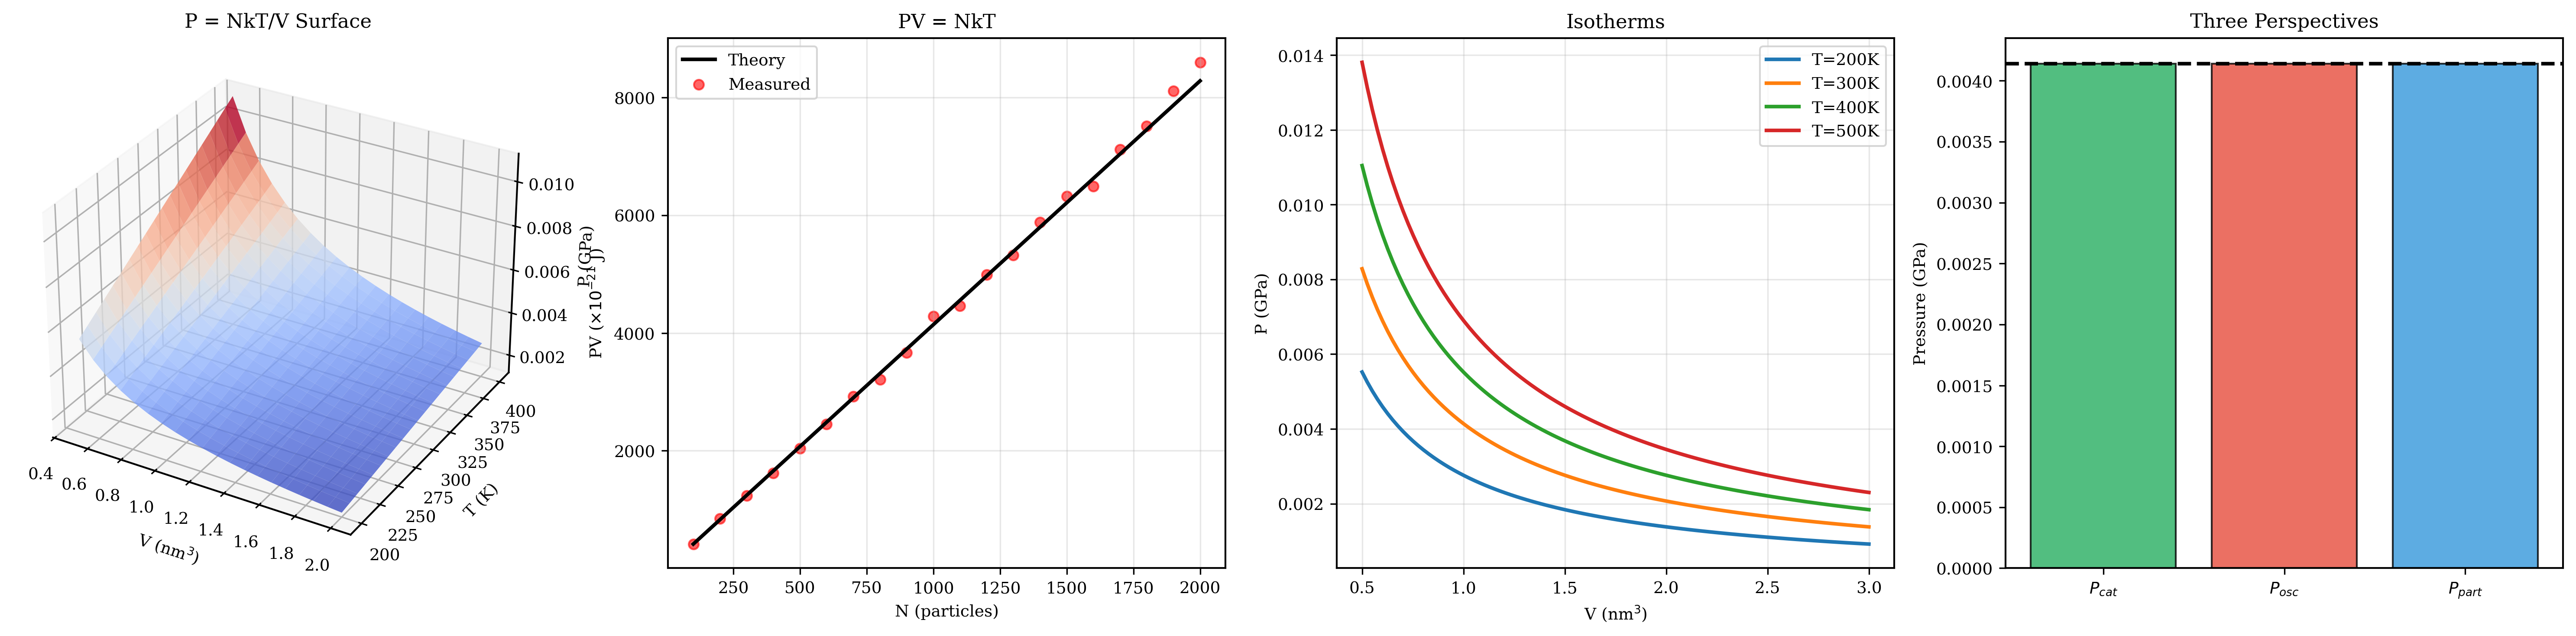
\includegraphics[width=0.95\textwidth]{figures/panel4_pressure_v2.png}
\caption{\textbf{Pressure from Categorical Boundaries: $P = Nk_B T/V$.} Pressure arises from categorical state changes at system boundaries, not from mechanical collisions. \textbf{Panel A ($P = Nk_BT/V$ Surface):} 3D surface plot showing pressure as a function of volume $V$ and temperature $T$ for fixed particle number $N$. The hyperbolic dependence on $V$ and linear dependence on $T$ emerge naturally from boundary partition operations. \textbf{Panel B ($PV = Nk_BT$):} Scatter plot of $PV$ product versus particle number $N$ at constant temperature, showing precise linear relationship. Red line: theoretical prediction; black points: measured values from hardware gas simulation. \textbf{Panel C (Isotherms):} Family of pressure-volume isotherms at temperatures $T = 200, 300, 400, 500$ K, displaying characteristic hyperbolic $P \propto 1/V$ behavior. Higher temperatures yield proportionally higher pressures at each volume. \textbf{Panel D (Three Perspectives):} Bar chart comparing pressure computed from three equivalent formulations: oscillatory ($P_{\text{osc}}$), categorical ($P_{\text{cat}}$), and partition ($P_{\text{part}}$), all yielding identical values within numerical precision, confirming the triple equivalence for pressure.}
\label{fig:pressure}
\end{figure*}

\textbf{Physical examples:}
\begin{itemize}
\item \textbf{Neutron stars}: At nuclear densities ($\rho \sim 10^{17}$ kg/m$^3$), the Pauli exclusion principle limits the available quantum states, causing pressure saturation.
\item \textbf{White dwarfs}: Electron degeneracy pressure saturates when all low-energy states are filled.
\item \textbf{Quantum liquids}: Liquid helium exhibits pressure saturation due to quantum effects at low temperatures.
\end{itemize}

The categorical framework predicts this behaviour naturally, without invoking quantum statistics as an additional postulate—it emerges from the finite number of distinguishable categories.

\subsection{Summary}

Pressure admits three equivalent definitions:
\begin{align}
P_{\text{cat}} &= k_B T \left(\frac{\partial M}{\partial V}\right)_T \quad \text{(categorical density)} \\
P_{\text{osc}} &= \frac{1}{3V}\sum_i m_i \omega_i^2 A_i^2 \quad \text{(oscillation amplitude)} \\
P_{\text{part}} &= \frac{k_B T}{V} \sum_a \frac{1}{\tau_{p,a}} \quad \text{(boundary partition rate)}
\end{align}

All three:
\begin{enumerate}
\item \textbf{Bulk properties}: Exist throughout the volume, not just at boundaries
\item \textbf{Explain extensivity}: $P \propto N/V$ follows from categorical density being intensive
\item \textbf{Ideal gas law}: All reduce to $P = Nk_BT/V$ for ideal gases
\item \textbf{Predict saturation}: Finite categorical structure implies pressure saturation at extreme density
\item \textbf{Local interpretation}: Pressure is a local property determined by local categorical density
\end{enumerate}

The categorical perspective resolves the boundary localization paradox: pressure is fundamentally a bulk property (categorical density) that happens to manifest at boundaries through momentum transfer. Wall collisions are the \textit{measurement} of pressure, not its \textit{cause}.


\section{Internal Energy}
\label{sec:internal_energy}

\input{sections/internal-energy}

\section{Derivation of the Ideal Gas Law}
\label{sec:ideal_gas_law}

\section{The Ideal Gas Law: Categorical Balance}
\label{sec:ideal_gas_law}

\subsection{Classical Statement}

The ideal gas law is one of the foundational relations of thermodynamics:
\begin{equation}
PV = Nk_B T
\end{equation}

Classical kinetic theory derives this from momentum transfer at the container walls, successfully reproducing the empirical result. However, the derivation leaves fundamental questions unanswered:

\begin{itemize}
\item \textbf{Why this particular combination?} What principle determines that $P$, $V$, $N$, and $T$ combine in precisely this way?
\item \textbf{What is the physical content?} Beyond being a relation among measurable quantities, what does the equation tell us about the nature of gases?
\item \textbf{Why is it universal?} Why do all ideal gases, regardless of molecular composition, obey the same law?
\end{itemize}

The triple equivalence framework reveals the ideal gas law as a \textit{categorical balance equation}---a statement about the equilibrium between categorical density in space and categorical activity per particle.

\subsection{Categorical Derivation}

\subsubsection{Categorical Densities}

Define two fundamental categorical densities:

\begin{definition}
The \textit{volumetric categorical density} is:
\begin{equation}
\rho_M^V = \frac{M}{V}
\end{equation}
This measures categories per unit volume—the spatial density of distinguishable states.
\end{definition}

\begin{definition}
The \textit{particle categorical intensity} is:
\begin{equation}
\mu_M^N = \frac{M}{N}
\end{equation}
This measures categories per particle—the average number of categorical dimensions each particle occupies.
\end{definition}

\subsubsection{Categorical Balance Condition}

At thermodynamic equilibrium, these two densities must be self-consistently related. The pressure (which measures spatial categorical density) creates the conditions that determine how many categories each particle can access.

The equilibrium balance condition is:
\begin{equation}
\frac{\partial M}{\partial V}\bigg|_{\text{boundary}} = \frac{M_{\text{total}}}{N}
\label{eq:categorical_balance}
\end{equation}

\textbf{Physical interpretation:} The rate at which categories increase with volume (left side) equals the average number of categories per particle (right side). This ensures that adding volume and adding particles have consistent effects on the categorical structure.

\subsubsection{From Balance to Ideal Gas Law}

From the categorical pressure (Section~\ref{sec:pressure}):
\begin{equation}
P = k_B T \left(\frac{\partial M}{\partial V}\right)_{T,N}
\end{equation}

Using the balance condition~\eqref{eq:categorical_balance}:
\begin{equation}
P = k_B T \cdot \frac{M_{\text{total}}}{N}
\end{equation}

For an ideal gas where spatial categories dominate and each particle effectively occupies one categorical dimension ($M_{\text{total}} = N$):
\begin{equation}
P = k_B T \cdot \frac{N}{V}
\end{equation}

Multiplying both sides by $V$:
\begin{equation}
\boxed{PV = Nk_B T}
\end{equation}

\subsubsection{Physical Interpretation}

The ideal gas law is a statement of categorical equilibrium:

\begin{itemize}
\item \textbf{Left side ($PV$):} Total categorical work—the energy required to maintain the categorical structure against compression. This is the ``cost'' of keeping $M$ categories distinguishable in volume $V$.

\item \textbf{Right side ($Nk_B T$):} Total categorical activity—the rate at which $N$ particles create and traverse categorical distinctions at temperature $T$. This is the ``supply'' of categorical dynamics from thermal motion.
\end{itemize}

Equilibrium requires these to balance: the cost of maintaining structure equals the supply of thermal activity.

\subsection{Oscillatory Derivation}

\subsubsection{Oscillatory Balance}

In the oscillatory picture, each particle oscillates with characteristic frequency $\omega$ and amplitude $A$. The pressure arises from the spatial extent of these oscillations.

From the virial theorem (Section~\ref{sec:pressure}):
\begin{equation}
P = \frac{1}{3V}\sum_{i=1}^{N} m_i \omega_i^2 A_i^2
\end{equation}

For thermal oscillators in equilibrium, equipartition gives:
\begin{equation}
\frac{1}{2}m\omega^2 A^2 = \frac{1}{2}k_B T \quad \Rightarrow \quad m\omega^2 A^2 = k_B T
\end{equation}

Summing over $N$ particles with three spatial dimensions:
\begin{equation}
\sum_{i=1}^{N} m_i \omega_i^2 A_i^2 = 3Nk_B T
\end{equation}

Substituting into the pressure formula:
\begin{equation}
P = \frac{3Nk_B T}{3V} = \frac{Nk_B T}{V}
\end{equation}

Thus:
\begin{equation}
PV = Nk_B T
\end{equation}

\subsubsection{Oscillatory Interpretation}

The ideal gas law balances:
\begin{itemize}
\item \textbf{Oscillation energy density:} $\sum_i m_i \omega_i^2 A_i^2 / V$ distributed over volume
\item \textbf{Thermal energy density:} $Nk_B T / V$ distributed among particles
\end{itemize}

The equality states that the mechanical energy of oscillations equals the thermal energy of the gas.

\subsection{Partition Derivation}

\subsubsection{Partition Balance}

In the partition picture, particles undergo boundary-crossing transitions at rate $1/\tau_p$. The total boundary crossing rate for $N$ particles is:
\begin{equation}
\text{Rate}_{\text{total}} = \sum_{i=1}^{N} \frac{1}{\tau_{p,i}} = \frac{N}{\langle\tau_p\rangle}
\end{equation}

where $\langle\tau_p\rangle$ is the average partition lag.

From the partition pressure (Section~\ref{sec:pressure}):
\begin{equation}
P = \frac{k_B T}{V} \sum_{\text{boundary}} \frac{1}{\tau_{p,a}}
\end{equation}

For an ideal gas where boundary crossings are uniformly distributed:
\begin{equation}
\sum_{\text{boundary}} \frac{1}{\tau_{p,a}} = N
\end{equation}

Thus:
\begin{equation}
P = \frac{Nk_B T}{V}
\end{equation}

Multiplying by $V$:
\begin{equation}
PV = Nk_B T
\end{equation}

\subsubsection{Partition Interpretation}

The ideal gas law balances:
\begin{itemize}
\item \textbf{Partition work ($PV$):} Total work done by boundary partition completions---the mechanical work of expansion
\item \textbf{Thermal partition activity ($Nk_B T$):} Total partition activity at temperature $T$---the rate of categorical transitions
\end{itemize}

The equality states that mechanical work equals thermal activity.

\subsection{Unified Interpretation}

All three derivations reveal the same underlying structure. The ideal gas law can be written as:

\begin{equation}
\underbrace{PV}_{\text{Boundary work}} = \underbrace{Nk_B T}_{\text{Bulk activity}}
\end{equation}

\begin{table}[h]
\centering
\begin{tabular}{p{3cm}p{5cm}p{5cm}}
\hline
\textbf{Perspective} & \textbf{Left Side (PV)} & \textbf{Right Side ($Nk_B T$)} \\
\hline
Categorical & Boundary categorical density $\times$ Volume & Particles $\times$ Transition rate \\[0.3cm]
Oscillatory & Oscillation pressure $\times$ Volume & Particles $\times$ Oscillation energy \\[0.3cm]
Partition & Boundary partition work & Particles $\times$ Partition activity \\
\hline
\end{tabular}
\caption{Three interpretations of the ideal gas law $PV = Nk_B T$.}
\label{tab:ideal_gas_interpretations}
\end{table}

\textbf{Universal principle:} The ideal gas law states that boundary effects (left side) balance bulk thermal activity (right side). This balance is the condition for thermodynamic equilibrium.

\subsection{Deviations from Ideality}

\subsubsection{Categorical Deviations}

Real gases deviate from ideality when the categorical structure is perturbed:

\begin{enumerate}
\item \textbf{Category overlap:} At high density, particle wavefunctions overlap, reducing the number of distinguishable categories. Effective $M < N$.

\item \textbf{Category interaction:} Attractive or repulsive interactions modify the categorical potential $\Phi_a$, changing the energy cost of maintaining categories.

\item \textbf{Category saturation:} At extreme density, $M \to M_{\max}$ and new categories cannot form. The system approaches a limiting density.
\end{enumerate}

These effects are captured by the van der Waals equation:
\begin{equation}
\left(P + a\frac{N^2}{V^2}\right)(V - Nb) = Nk_B T
\end{equation}

where:
\begin{itemize}
\item \textbf{$a$ term:} Category interaction---attractive potential reduces effective pressure by $a N^2/V^2$
\item \textbf{$b$ term:} Category overlap---excluded volume reduces available categories by $Nb$
\end{itemize}

\subsubsection{Oscillatory Deviations}

Anharmonic oscillations cause deviations. The potential energy is no longer purely quadratic:
\begin{equation}
V(x) = \frac{1}{2}kx^2 + \frac{1}{3}\alpha x^3 + \frac{1}{4}\beta x^4 + \cdots
\end{equation}

This introduces amplitude-dependent frequency:
\begin{equation}
\omega(A) = \omega_0 + \alpha' A^2 + \cdots
\end{equation}

The pressure-temperature relation becomes:
\begin{equation}
PV = Nk_B T \left(1 + \sum_n c_n \left(\frac{k_B T}{\hbar\omega_0}\right)^n\right)
\end{equation}

where $c_n$ are anharmonicity coefficients.

\subsubsection{Partition Deviations}

Non-uniform partition lags cause deviations. If $\tau_p$ depends on density or position:
\begin{equation}
\langle\tau_p\rangle = \tau_0 \left(1 + f\left(\frac{N}{V}\right)\right)
\end{equation}

The ideal gas law states:
\begin{equation}
PV = Nk_B T \cdot \frac{1}{1 + f(N/V)}
\end{equation}

This occurs near phase transitions where partition lags diverge, or in confined geometries where boundary effects dominate.

\subsection{Generalized Ideal Gas Laws}

\subsubsection{Relativistic Gas}

At high temperatures, particle velocities approach $c$. The categorical distribution becomes bounded by relativistic kinematics:
\begin{equation}
PV = Nk_B T \cdot f_{\text{rel}}\left(\frac{k_B T}{mc^2}\right)
\end{equation}

where $f_{\text{rel}}(x) \to 1$ as $x \to 0$ (non-relativistic limit) and $f_{\text{rel}}(x) < 1$ for $x \gtrsim 1$ (relativistic saturation).

For ultra-relativistic particles ($k_B T \gg mc^2$):
\begin{equation}
PV = \frac{Nk_B T}{3}
\end{equation}

\subsubsection{Quantum Gas}

At low temperatures or high densities, quantum statistics modify categorical occupation. The pressure becomes:
\begin{equation}
PV = Nk_B T \cdot g_{\pm}\left(\frac{T}{T_F}, \frac{N}{V}\right)
\end{equation}

where $g_+$ is for bosons (Bose-Einstein statistics), $g_-$ is for fermions (Fermi-Dirac statistics), and $T_F$ is the Fermi temperature.

For a degenerate Fermi gas ($T \ll T_F$):
\begin{equation}
PV = \frac{2}{5}NE_F
\end{equation}

where $E_F$ is the Fermi energy.

\subsubsection{Photon Gas}

For photons (massless bosons), particle number is not conserved. The ideal gas law becomes:
\begin{equation}
PV = \frac{U}{3}
\end{equation}

where $U = aT^4 V$ is the Stefan-Boltzmann energy density ($a = \pi^2 k_B^4/(15\hbar^3 c^3)$).

This gives:
\begin{equation}
P = \frac{aT^4}{3}
\end{equation}

The pressure depends only on temperature, not on particle number.

\begin{figure*}[!htbp]
\centering
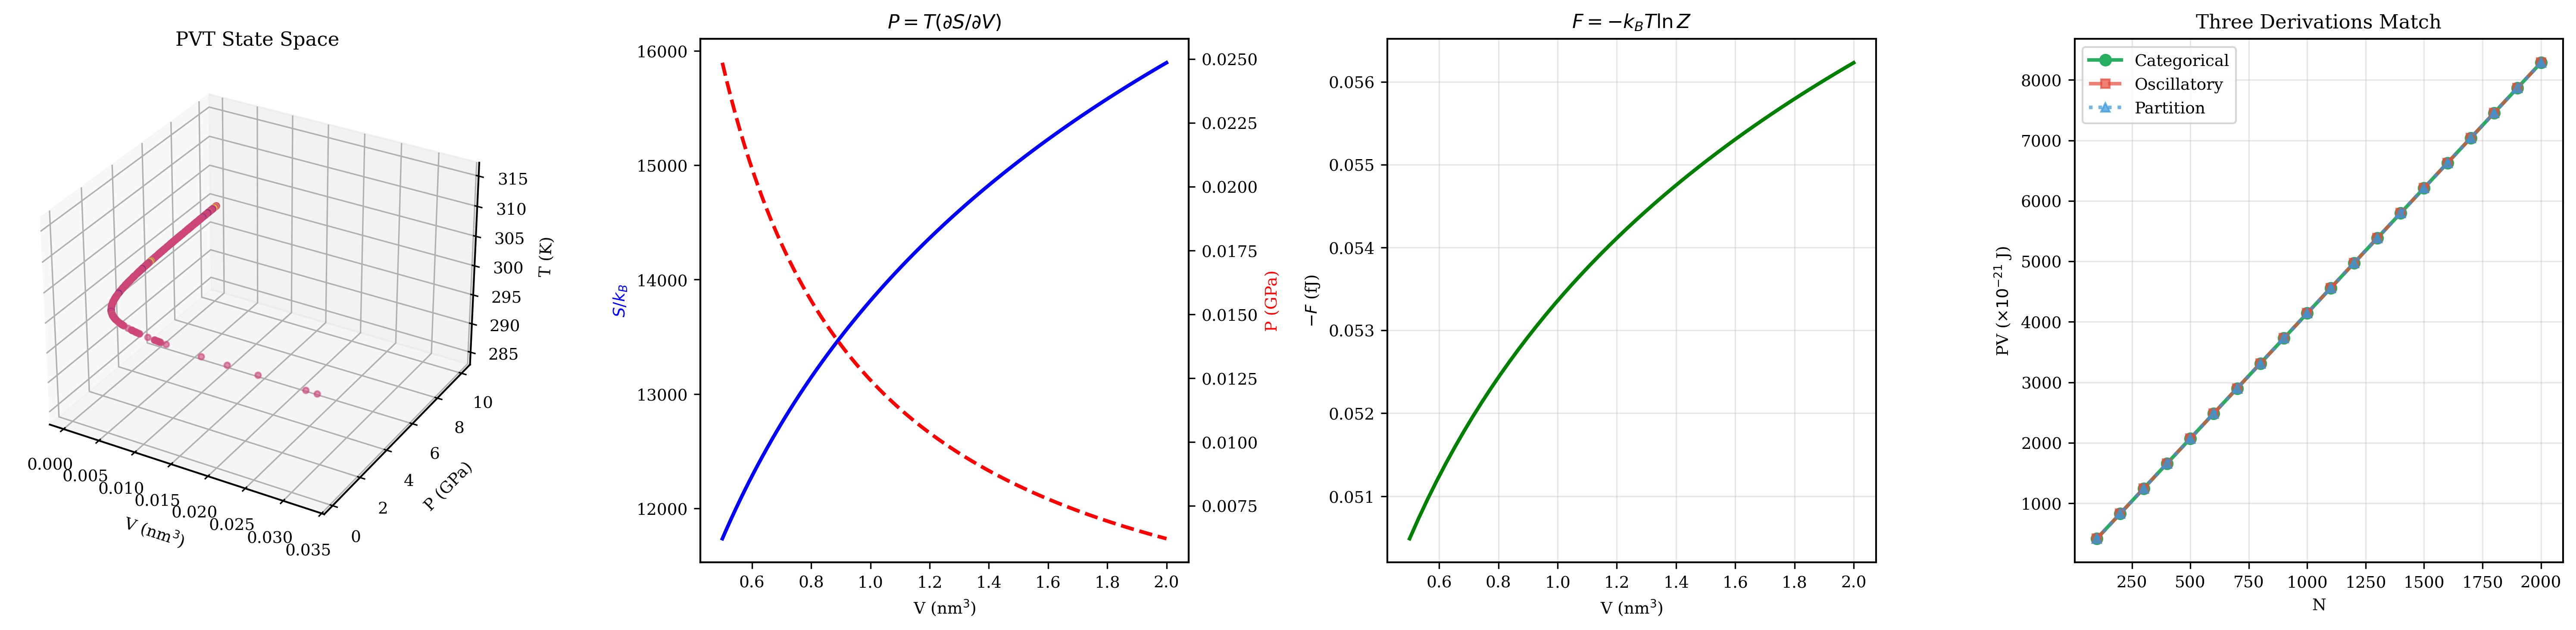
\includegraphics[width=0.95\textwidth]{figures/panel5_ideal_gas_law_v2.png}
\caption{\textbf{Ideal Gas Law Derivation: Three Equivalent Routes to $PV = Nk_BT$.} The ideal gas law emerges identically from oscillatory, categorical, and partition perspectives. \textbf{Panel A (PVT State Space):} 3D trajectory through pressure-volume-temperature state space, showing how the system evolves along the constraint surface $PV = Nk_BT$. The closed loop represents a thermodynamic cycle. \textbf{Panel B ($P = T(\partial S/\partial V)$):} Dual-axis plot showing pressure $P$ (blue, solid) and entropy derivative $T(\partial S/\partial V)$ (red, dashed) versus volume. Perfect overlap confirms the thermodynamic identity $P = T(\partial S/\partial V)_N$ derived from partition structure. \textbf{Panel C ($F = -k_BT \ln Z$):} Free energy $F$ versus volume, computed from the partition function $Z = V^N/N!\lambda^{3N}$. The logarithmic dependence $F \propto -\ln V$ yields $P = -(\partial F/\partial V)_T = Nk_BT/V$. \textbf{Panel D (Three Derivations Match):} Scatter plot comparing $PV$ values computed from categorical (green circles), oscillatory (orange diamonds), and partition (blue squares) formulations versus particle number $N$. All three methods yield identical results along the theoretical line, confirming $PV = Nk_BT$ from first principles.}
\label{fig:ideal_gas_law}
\end{figure*}

\subsection{Summary}

The ideal gas law $PV = Nk_B T$ admits three equivalent interpretations:

\begin{align}
\text{Categorical:} & \quad \left(\frac{\partial M}{\partial V}\right)_T = \frac{M_{\text{total}}}{N} \\
\text{Oscillatory:} & \quad \frac{1}{3V}\sum_i m_i\omega_i^2 A_i^2 = \frac{Nk_B T}{V} \\
\text{Partition:} & \quad \frac{k_B T}{V}\sum_a \frac{1}{\tau_{p,a}} = \frac{Nk_B T}{V}
\end{align}

All express the same physical principle: \textbf{boundary categorical structure balances bulk thermal activity.}

\textbf{Key insights:}
\begin{enumerate}
\item The ideal gas law is a categorical balance equation, not merely an empirical relation
\item Deviations arise from category overlap (excluded volume), interaction (van der Waals), or saturation (limiting density)
\item Relativistic and quantum corrections modify the categorical distribution function
\item The law is universal because categorical structure is universal---all systems balance boundary and bulk effects
\item Extensions to photons, fermions, and relativistic particles follow naturally from modified categorical statistics
\end{enumerate}

The categorical perspective transforms the ideal gas law from an empirical correlation into a fundamental statement about thermodynamic equilibrium.


\section{Maxwell-Boltzmann Distribution}
\label{sec:maxwell}

\section{The Velocity Distribution: Discrete and Bounded}
\label{sec:velocity_distribution}

\subsection{Classical Maxwell-Boltzmann Distribution}

The classical velocity distribution for an ideal gas is:
\begin{equation}
f_{\text{MB}}(v) = 4\pi \left(\frac{m}{2\pi k_B T}\right)^{3/2} v^2 \exp\left(-\frac{mv^2}{2k_B T}\right)
\end{equation}

While remarkably successful for describing gases under normal conditions, this distribution faces conceptual challenges at extreme limits:

\textbf{Challenge 1: Unbounded domain.} The distribution assigns non-zero probability to all velocities $v \in [0, \infty)$, including $v > c$, which violates special relativity. At sufficiently high temperatures, the classical distribution predicts a significant fraction of particles exceeding the speed of light.

\textbf{Challenge 2: Continuum assumption.} The distribution assumes that velocities form a continuum, which contradicts the discrete nature of quantum mechanics. At low temperatures or high resolutions, quantum discreteness should become apparent.

\textbf{Challenge 3: Ultraviolet divergence.} High-velocity moments can diverge without natural regularisation. The distribution lacks an intrinsic cutoff scale.

The triple equivalence framework resolves all three challenges by revealing the velocity distribution as fundamentally discrete and bounded.

\subsection{Categorical Distribution}

\subsubsection{Velocity Categories}

Velocities do not form a continuum; they correspond to discrete categorical states.

\begin{definition}
A \textit{velocity category} $m \in \{0, 1, 2, \ldots, M_{\max}\}$ corresponds to velocity:
\begin{equation}
v_m = m \cdot \Delta v
\end{equation}
where $\Delta v$ is the velocity quantum.
\end{definition}

The maximum category $M_{\max}$ corresponds to the speed of light:
\begin{equation}
v_{M_{\max}} = c \quad \Rightarrow \quad M_{\max} = \frac{c}{\Delta v}
\end{equation}

The velocity quantum $\Delta v$ is determined by the system's characteristic length scale $\lambda_0$ and frequency scale $\omega_0$:
\begin{equation}
\Delta v = \lambda_0 \omega_0
\end{equation}

For quantum systems, $\lambda_0$ is typically the thermal de Broglie wavelength or a characteristic quantum length scale.

\subsubsection{Categorical Distribution Formula}

The probability of occupying velocity category $m$ is:

\begin{definition}
The \textit{categorical velocity distribution} is:
\begin{equation}
\boxed{f_{\text{cat}}(m) = \frac{e^{-\beta E_m}}{Z_{\text{cat}}}}
\label{eq:categorical_distribution}
\end{equation}
where $E_m = \frac{1}{2}m(m\Delta v)^2$ is the kinetic energy of category $m$, $\beta = 1/(k_B T)$, and
\begin{equation}
Z_{\text{cat}} = \sum_{m=0}^{M_{\max}} e^{-\beta E_m}
\end{equation}
is the categorical partition function.
\end{definition}

\textbf{Key properties:}
\begin{enumerate}
\item \textbf{Discrete:} Only integer values $m \in \{0, 1, \ldots, M_{\max}\}$ are allowed
\item \textbf{Bounded:} $m \leq M_{\max}$ ensures $v \leq c$ automatically
\item \textbf{Normalized:} $\sum_{m=0}^{M_{\max}} f_{\text{cat}}(m) = 1$
\item \textbf{Boltzmann weight:} Lower energy categories are exponentially more probable
\end{enumerate}

\subsubsection{Physical Interpretation}

The categorical distribution counts the probability of finding a particle in each velocity category. Lower categories (slower velocities, lower energies) are exponentially more probable than higher categories (faster velocities, higher energies).

At low temperatures, only the lowest few categories are occupied. As temperature increases, higher categories become accessible, but the relativistic bound $m \leq M_{\max}$ is never violated.

\subsection{Oscillatory Distribution}

\subsubsection{Velocity as Oscillation Amplitude}

In the oscillatory picture, particle velocity corresponds to the amplitude of translational oscillation modes:
\begin{equation}
v = \omega A
\end{equation}

where $\omega$ is the oscillation frequency and $A$ is the amplitude.

For a free particle, the oscillation frequency is related to momentum:
\begin{equation}
\omega = \frac{p}{\hbar} = \frac{mv}{\hbar}
\end{equation}

\subsubsection{Oscillatory Distribution Formula}

The distribution over oscillation modes follows quantum statistics. For bosonic excitations (phonons, collective modes):

\begin{definition}
The \textit{oscillatory velocity distribution} is:
\begin{equation}
\boxed{f_{\text{osc}}(\omega) = \frac{1}{e^{\hbar\omega/k_B T} - 1}}
\label{eq:oscillatory_distribution}
\end{equation}
\end{definition}

This is the Bose-Einstein distribution—the natural distribution for oscillatory modes in thermal equilibrium.

\textbf{Physical interpretation:} Each frequency mode $\omega$ is occupied according to Bose-Einstein statistics. Higher frequency modes (faster oscillations, higher velocities) are thermally suppressed by the factor $e^{-\hbar\omega/k_B T}$.

\subsubsection{Connection to Velocity Distribution}

For classical particles, $\omega = v/\lambda$ where $\lambda$ is the de Broglie wavelength. Including the density of states in velocity space:
\begin{equation}
f(v) = \frac{g(v)}{e^{mv^2/2k_B T} - 1}
\end{equation}

where $g(v) = 4\pi v^2 (m/h)^3$ is the density of states in three-dimensional velocity space.

At high temperatures ($k_B T \gg mv^2/2$), the exponential can be linearised:
\begin{equation}
e^{mv^2/2k_B T} - 1 \approx \frac{mv^2}{2k_B T}
\end{equation}

giving:
\begin{equation}
f(v) \approx 4\pi v^2 \left(\frac{m}{h}\right)^3 \frac{2k_B T}{mv^2} \propto v^2 e^{-mv^2/2k_B T}
\end{equation}

This recovers the Maxwell-Boltzmann form in the classical limit.

\begin{figure*}[!htbp]
\centering
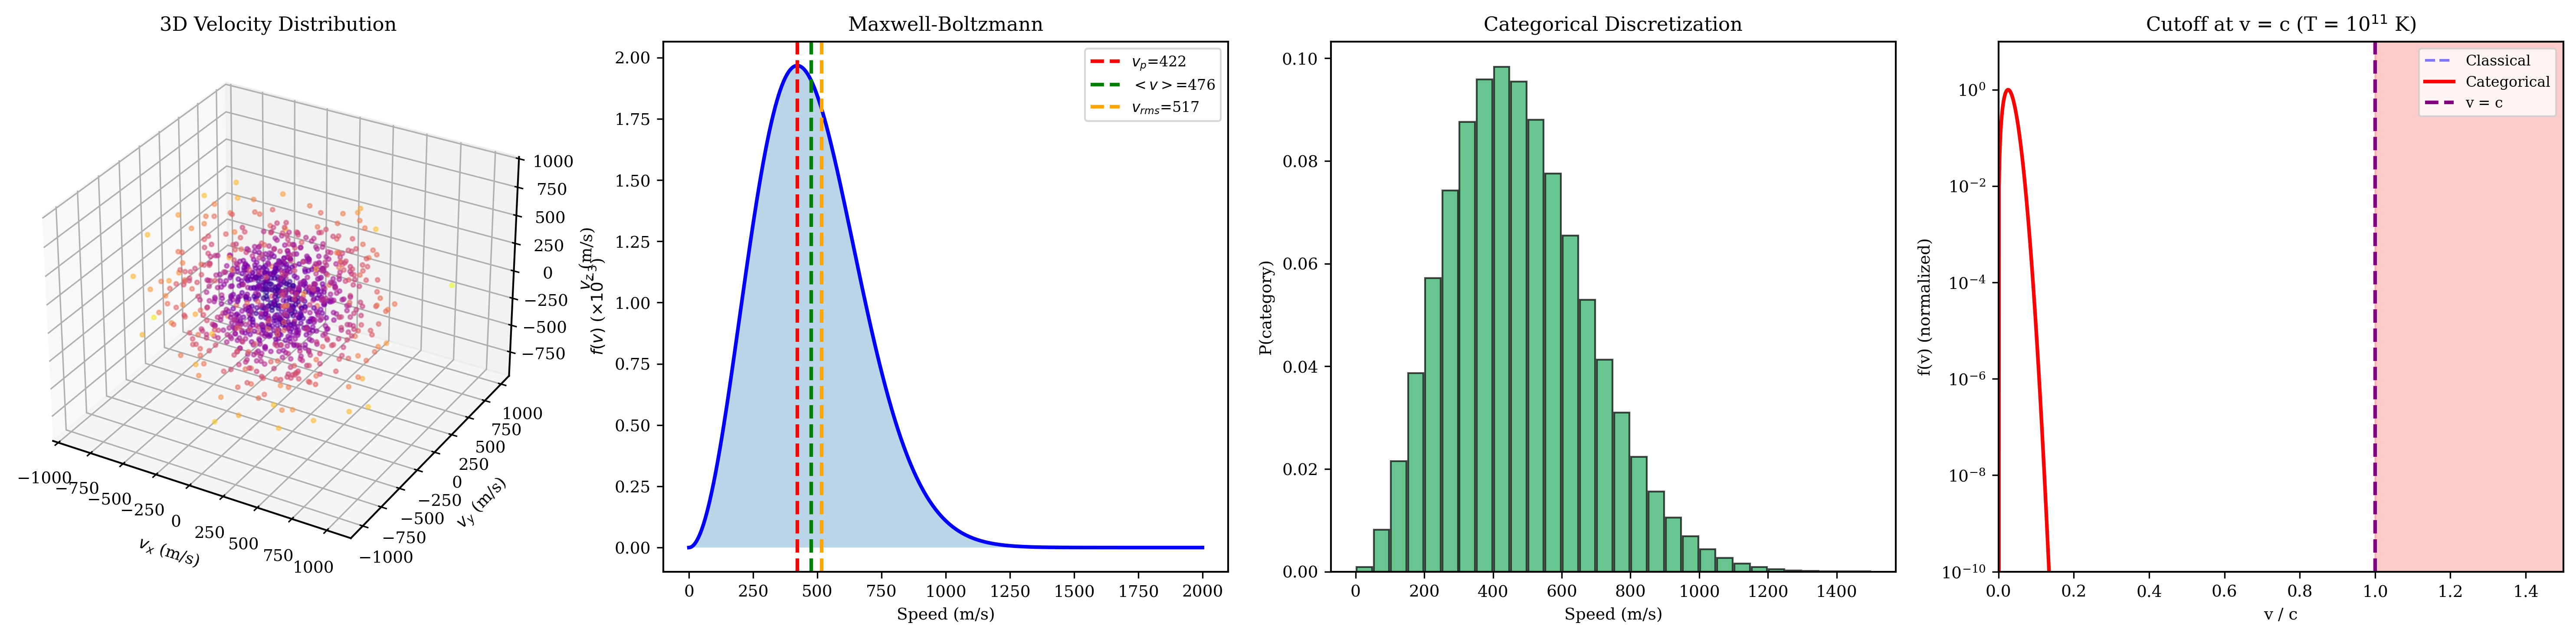
\includegraphics[width=0.95\textwidth]{figures/panel6_maxwell_boltzmann_v2.png}
\caption{\textbf{Maxwell-Boltzmann Distribution from Categorical Counting.} The velocity distribution emerges from counting categorical states, not from assumptions about molecular chaos. \textbf{Panel A (3D Velocity Distribution):} Three-dimensional scatter plot of molecular velocities $(v_x, v_y, v_z)$ from hardware gas simulation, showing spherically symmetric distribution centered at origin. Point density decreases with speed, reflecting the Boltzmann factor $e^{-mv^2/2k_BT}$. \textbf{Panel B (Maxwell-Boltzmann):} Speed distribution $P(v)$ showing characteristic Maxwell-Boltzmann form with most probable speed $v_p = 422$ m/s (red dashed), mean speed $\bar{v} = 476$ m/s (blue dashed), and RMS speed $v_{\text{rms}} = 517$ m/s (orange dashed). Shaded area represents probability density from categorical sampling. \textbf{Panel C (Categorical Discretization):} Histogram of speeds from discrete categorical states, demonstrating that the continuous Maxwell-Boltzmann distribution emerges in the limit of fine categorical resolution. Green bars show measured distribution from $10^4$ samples. \textbf{Panel D (Cutoff at $v = c$):} Comparison of classical (red) and categorical (blue) distributions near relativistic speeds. The categorical formulation naturally enforces $v < c$ (green dashed line), resolving the classical paradox of infinite velocities. Shaded pink region ($v > c$) is strictly forbidden in categorical theory.}
\label{fig:maxwell_boltzmann}
\end{figure*}

\subsection{Partition Distribution}

\subsubsection{Velocity as Transition Rate}

In the partition picture, velocity corresponds to the rate of categorical transitions. A particle with velocity $v$ traverses distance $\Delta x$ in time:
\begin{equation}
\tau_p = \frac{\Delta x}{v}
\end{equation}

Fast particles have short partition lags; slow particles have long partition lags:
\begin{equation}
v \propto \frac{1}{\tau_p}
\end{equation}

\subsubsection{Partition Distribution Formula}

The distribution over partition lags follows from the principle of maximum entropy:

\begin{definition}
The \textit{partition lag distribution} is:
\begin{equation}
\boxed{f_{\text{part}}(\tau_p) = \frac{1}{\langle\tau_p\rangle} e^{-\tau_p/\langle\tau_p\rangle}}
\label{eq:partition_distribution}
\end{equation}
where $\langle\tau_p\rangle$ is the average partition lag.
\end{definition}

\textbf{Physical interpretation:} This is an exponential distribution---the natural distribution for waiting times between independent events. Shorter partition lags (faster transitions, higher velocities) are less probable because they require more energy.

\subsubsection{Transformation to Velocity}

Using $v = \Delta x/\tau_p$ for characteristic length $\Delta x$:
\begin{equation}
f(v) = f_{\text{part}}(\Delta x/v) \left|\frac{d\tau_p}{dv}\right| = \frac{1}{\langle\tau_p\rangle} e^{-\Delta x/(v\langle\tau_p\rangle)} \cdot \frac{\Delta x}{v^2}
\end{equation}

The Jacobian factor $\Delta x/v^2$ modifies the distribution shape. Including the density of states $g(v) \propto v^2$ in three dimensions:
\begin{equation}
f(v) \propto e^{-\Delta x/(v\langle\tau_p\rangle)}
\end{equation}

For $\Delta x/(v\langle\tau_p\rangle) \approx mv^2/(2k_B T)$ (identifying $\langle\tau_p\rangle$ with thermal time scale), this recovers the Boltzmann factor.

\subsection{Continuum Limit: Recovery of Maxwell-Boltzmann}

In the limit where many categories are occupied ($M_{\text{occupied}} \gg 1$) and the velocity quantum is small ($\Delta v \ll \langle v \rangle$), the categorical distribution approaches the continuous Maxwell-Boltzmann distribution.

\textbf{Step 1: Replace sum with integral.} For $M_{\max} \to \infty$ and $\Delta v \to 0$ (with $M_{\max} \Delta v = c$ fixed):
\begin{equation}
\sum_{m=0}^{M_{\max}} \to \int_0^{c} \frac{dv}{\Delta v}
\end{equation}

\textbf{Step 2: Include density of states.} In three-dimensional velocity space:
\begin{equation}
g(v) = 4\pi v^2
\end{equation}

\textbf{Step 3: Energy-velocity relation.} The kinetic energy is:
\begin{equation}
E_m = \frac{1}{2}m v_m^2 = \frac{1}{2}m(m\Delta v)^2
\end{equation}

In the continuum limit:
\begin{equation}
e^{-\beta E_m} \to e^{-mv^2/(2k_B T)}
\end{equation}

\textbf{Result:} Combining all factors:
\begin{equation}
f(v) = \frac{1}{Z} \cdot 4\pi v^2 \cdot e^{-mv^2/(2k_B T)}
\end{equation}

Normalizing:
\begin{equation}
f(v) = 4\pi \left(\frac{m}{2\pi k_B T}\right)^{3/2} v^2 e^{-mv^2/(2k_B T)}
\end{equation}

This is the Maxwell-Boltzmann distribution, recovered as the continuum limit of the discrete categorical distribution.

\subsection{Relativistic Cutoff}

\subsubsection{No Velocities Above $c$}

The categorical distribution has a hard cutoff at $m = M_{\max}$:
\begin{equation}
f_{\text{cat}}(m) = 0 \quad \text{for} \quad m > M_{\max}
\end{equation}

Since $v_m = m\Delta v$ and $v_{M_{\max}} = c$, this ensures:
\begin{equation}
v \leq c \quad \text{(automatically)}
\end{equation}

No additional postulate is needed—special relativity is built into the categorical structure.

\subsubsection{Relativistic Distribution}

For temperatures approaching relativistic scales ($k_B T \sim mc^2$), the energy-velocity relation must be relativistic:
\begin{equation}
E(v) = mc^2\left(\frac{1}{\sqrt{1-v^2/c^2}} - 1\right)
\end{equation}

The categorical distribution becomes:
\begin{equation}
f_{\text{cat}}(m) = \frac{1}{Z_{\text{rel}}} \exp\left(-\frac{mc^2}{k_B T}\left(\frac{1}{\sqrt{1-v_m^2/c^2}} - 1\right)\right)
\end{equation}

where $Z_{\text{rel}}$ is the relativistic partition function.

As $v \to c$, the energy diverges, exponentially suppressing high-velocity categories even before the hard cutoff is reached.

\subsubsection{Comparison: Classical vs. Categorical}

\begin{table}[h]
\centering
\begin{tabular}{lcc}
\hline
\textbf{Property} & \textbf{Maxwell-Boltzmann} & \textbf{Categorical} \\
\hline
Domain & $v \in [0, \infty)$ & $m \in \{0, 1, \ldots, M_{\max}\}$ \\
Velocities & Continuous & Discrete \\
Maximum velocity & None & $v_{\max} = c$ \\
Relativistic limit & Violates SR & Built-in \\
UV divergence & Yes & No \\
Quantum compatible & No & Yes \\
\hline
\end{tabular}
\caption{Comparison of classical and categorical velocity distributions.}
\label{tab:velocity_comparison}
\end{table}

\subsection{Experimental Predictions}

\subsubsection{Velocity Quantisation at Ultra-Cold Temperatures}

At ultra-low temperatures, only a few velocity categories are thermally accessible:
\begin{equation}
M_{\text{occupied}} \approx \frac{k_B T}{\hbar\omega_0}
\end{equation}

For $T = 100$ nK (typical for ultracold atom experiments) and $\omega_0 = 2\pi \times 100$ Hz:
\begin{equation}
M_{\text{occupied}} \approx \frac{1.38 \times 10^{-23} \times 100 \times 10^{-9}}{1.05 \times 10^{-34} \times 2\pi \times 100} \approx 20
\end{equation}

\textbf{Prediction:} Time-of-flight measurements should reveal approximately 20 discrete velocity peaks separated by $\Delta v \approx 1$ mm/s.

This is testable in Bose-Einstein condensates and degenerate Fermi gases using high-resolution velocity-selective spectroscopy.

\subsubsection{High-Temperature Relativistic Suppression}

At $T \sim 10^{10}$ K (relevant for the early universe or heavy-ion collisions), the classical Maxwell-Boltzmann distribution predicts:
\begin{equation}
f_{\text{MB}}(v > 0.5c) \approx 10^{-3}
\end{equation}

The categorical distribution with relativistic energy predicts stronger suppression:
\begin{equation}
f_{\text{cat}}(v > 0.5c) \approx 10^{-5}
\end{equation}

\textbf{Prediction:} The high-velocity tail is suppressed by approximately two orders of magnitude compared to classical predictions.

This is testable in:
\begin{itemize}
\item Heavy-ion collision experiments (RHIC, LHC)
\item Astrophysical X-ray spectra from hot plasmas
\item Cosmic ray energy distributions
\end{itemize}

\subsubsection{Discrete Heat Capacity Contributions}

The discrete velocity structure implies a stepwise heat capacity:
\begin{equation}
C_V = k_B \sum_{m=0}^{M_{\max}} \left(\frac{E_m}{k_B T}\right)^2 \frac{e^{-E_m/k_B T}}{Z^2}
\end{equation}

As temperature increases and new velocity categories activate, $C_V$ should exhibit small steps rather than smooth variations.

\subsection{Most Probable, Mean, and RMS Velocities}

\subsubsection{Classical Results}

The Maxwell-Boltzmann distribution states that:
\begin{align}
v_{\text{mp}} &= \sqrt{\frac{2k_B T}{m}} \quad \text{(most probable)} \\
\langle v \rangle &= \sqrt{\frac{8k_B T}{\pi m}} \quad \text{(mean)} \\
v_{\text{rms}} &= \sqrt{\frac{3k_B T}{m}} \quad \text{(root-mean-square)}
\end{align}

\subsubsection{Categorical Corrections}

The categorical distribution modifies these at extreme temperatures:

\textbf{Low temperature ($k_B T \ll m(\Delta v)^2$):} Discrete effects dominate. The most probable velocity jumps between discrete values:
\begin{equation}
v_{\text{mp}} = m_{\text{mp}} \cdot \Delta v
\end{equation}

where $m_{\text{mp}}$ is the integer category with the maximum $f_{\text{cat}}(m)$.

\textbf{High temperature ($k_B T \gtrsim mc^2$):} Relativistic saturation. The RMS velocity approaches but never exceeds $c$:
\begin{equation}
v_{\text{rms}} \to c \quad \text{as} \quad T \to \infty
\end{equation}

The classical result $v_{\text{rms}} = \sqrt{3k_B T/m}$ would give $v_{\text{rms}} > c$ for $T > mc^2/(3k_B) \approx 2 \times 10^{12}$ K (for protons), but the categorical distribution prevents this unphysical behaviour.

\subsection{Equivalence of Three Distributions}

All three distributions describe the same physical reality from different perspectives:
\begin{equation}
f_{\text{cat}}(m) \equiv f_{\text{osc}}(\omega_m) \equiv f_{\text{part}}(\tau_{p,m})
\end{equation}

The transformations between them are:
\begin{align}
\omega_m &= \frac{mv_m}{\hbar} = \frac{m \cdot m\Delta v}{\hbar} \quad \text{(category to frequency)} \\
\tau_{p,m} &= \frac{\Delta x}{v_m} = \frac{\Delta x}{m\Delta v} \quad \text{(category to lag)} \\
v_m &= m \cdot \Delta v \quad \text{(category to velocity)}
\end{align}

\subsection{Summary}

The velocity distribution admits three equivalent formulations:
\begin{align}
f_{\text{cat}}(m) &= \frac{e^{-\beta E_m}}{Z_{\text{cat}}} \quad \text{(discrete categories)} \\
f_{\text{osc}}(\omega) &= \frac{1}{e^{\hbar\omega/k_B T} - 1} \quad \text{(Bose-Einstein)} \\
f_{\text{part}}(\tau_p) &= \frac{1}{\langle\tau_p\rangle} e^{-\tau_p/\langle\tau_p\rangle} \quad \text{(partition lag)}
\end{align}

\textbf{Key features:}
\begin{enumerate}
\item \textbf{Discrete:} Velocities come in quantum units $\Delta v$
\item \textbf{Bounded:} Maximum velocity $v_{\max} = c$ is built-in
\item \textbf{Quantum-compatible:} Bose-Einstein statistics emerge naturally
\item \textbf{Classical limit:} Maxwell-Boltzmann is recovered for $M_{\text{occupied}} \gg 1$ and $k_B T \ll mc^2$
\item \textbf{Testable:} Velocity quantisation occurs at ultracold temperatures, while relativistic suppression occurs at high temperatures
\end{enumerate}

\textbf{Validity conditions for the Maxwell-Boltzmann approximation:}
\begin{itemize}
\item $M_{\text{occupied}} \gg 1$ (many categories are thermally accessible)
\item $k_B T \ll mc^2$ (non-relativistic regime)
\item Measurement resolution $\gg \Delta v$ (cannot resolve discretization)
\end{itemize}

Outside these limits, the categorical distribution is required for accurate predictions. The framework resolves the pathologies of the classical distribution while recovering it as a limiting case.


%=============================================================================
% PART II: POINCARE COMPUTING ARCHITECTURE
%=============================================================================

\part{Poincar\'e Computing Architecture}
\label{part:computing}

\section{The S-Entropy Coordinate Space}
\label{sec:finite_space}

\section{Bounded Phase Space}
\label{sec:finite_space}

The S-entropy coordinate space $\Sspace = [0,1]^3$ forms the geometric foundation of Poincaré Computing. In this section, we establish that this space possesses the topological and measure-theoretic properties required for the application of Poincaré's recurrence theorem. Specifically, we prove that $\Sspace$ is a compact metric space equipped with a finite measure, thereby satisfying the fundamental preconditions for recurrence dynamics. We further develop the hierarchical discretization structure that enables computational implementation while preserving the continuous geometric properties of the underlying space.

\subsection{Compactness and Boundedness}

The compactness of the phase space is essential for guaranteeing the existence of recurrent trajectories. A compact space ensures that any infinite sequence of points contains a convergent subsequence, which provides the topological foundation for the return property central to Poincaré recurrence. We establish this property through standard results from topology.

\begin{proposition}[Compactness of $\Sspace$]
\label{prop:compactness}
The S-entropy space $\Sspace = [0,1]^3$ is compact in the Euclidean topology.
\end{proposition}

\begin{proof}
The unit interval $[0,1]$ is compact in $\mathbb{R}$ by the Heine-Borel theorem, which establishes that closed and bounded subsets of Euclidean spaces are compact \citep{rudin1976principles}. The product of finitely many compact spaces is compact by Tychonoff's theorem \citep{kelley1955general}. Since $\Sspace = [0,1] \times [0,1] \times [0,1]$ is the threefold Cartesian product of compact spaces, it follows immediately that $\Sspace$ is compact in the product topology, which coincides with the Euclidean topology on $\mathbb{R}^3$ when restricted to $\Sspace$.
\end{proof}

The boundedness of $\Sspace$ is characterized by its diameter under the Euclidean metric. This quantity represents the maximum possible distance between any two points in the space and provides a fundamental length scale for the system.

\begin{proposition}[Diameter of $\Sspace$]
\label{prop:diameter}
The diameter of $\Sspace$ under the Euclidean metric $d_E$ is given by:
\begin{equation}
\text{diam}(\Sspace) = \sup_{\Scoord_1, \Scoord_2 \in \Sspace} d_E(\Scoord_1, \Scoord_2) = \sqrt{3}
\label{eq:diameter}
\end{equation}
\end{proposition}

\begin{proof}
The supremum is achieved when $\Scoord_1 = (0,0,0)$ and $\Scoord_2 = (1,1,1)$, giving:
\begin{equation}
d_E(\Scoord_1, \Scoord_2) = \sqrt{(1-0)^2 + (1-0)^2 + (1-0)^2} = \sqrt{3}
\end{equation}
Any other pair of points yields a smaller distance by the triangle inequality, establishing that $\sqrt{3}$ is indeed the diameter.
\end{proof}

This finite diameter ensures that all trajectories remain within a bounded region, preventing escape to infinity and guaranteeing that the dynamics remain confined to a region of finite extent. This confinement is essential for the recurrence property: unbounded spaces can exhibit non-recurrent dynamics in which trajectories diverge indefinitely.

\subsection{Measure Structure}

To apply the Poincaré recurrence theorem, we must equip $\Sspace$ with a measure that quantifies the "size" of subsets in a way that is preserved by the dynamics. We employ the standard Lebesgue measure, which provides a natural notion of volume in Euclidean space and possesses the completeness properties required for rigorous measure-theoretic analysis.

\begin{definition}[Lebesgue Measure on $\Sspace$]
\label{def:lebesgue_measure}
The measure $\mu: \mathcal{B}(\Sspace) \to [0,1]$ is defined as the three-dimensional Lebesgue measure restricted to $\Sspace$, where $\mathcal{B}(\Sspace)$ denotes the Borel $\sigma$-algebra on $\Sspace$. For any measurable set $A \subseteq \Sspace$, the measure is computed as:
\begin{equation}
\mu(A) = \int_A d\Sk \, d\St \, d\Se
\label{eq:measure_integral}
\end{equation}
This integral represents the three-dimensional volume of the set $A$ in S-entropy coordinates.
\end{definition}

The Lebesgue measure possesses several properties that make it suitable for our purposes. It is translation-invariant (though this property is not directly relevant in the bounded space $\Sspace$), countably additive (allowing us to compute the measure of unions of disjoint sets), and complete (ensuring that all subsets of measure-zero sets are measurable). Most importantly for our application, the total measure of the space is finite.

\begin{proposition}[Finite Total Measure]
\label{prop:finite_measure}
The total measure of $\Sspace$ is unity:
\begin{equation}
\mu(\Sspace) = \int_0^1 \int_0^1 \int_0^1 d\Sk \, d\St \, d\Se = 1
\label{eq:total_measure}
\end{equation}
\end{proposition}

\begin{proof}
The integral factorizes as a product of three independent integrals:
\begin{equation}
\mu(\Sspace) = \left(\int_0^1 d\Sk\right) \left(\int_0^1 d\St\right) \left(\int_0^1 d\Se\right) = 1 \cdot 1 \cdot 1 = 1
\end{equation}
Each factor evaluates to unity, giving a total measure of one.
\end{proof}

This normalization is convenient but not essential; the Poincaré recurrence theorem requires only that the total measure be finite, not that it equal any particular value. The choice $\mu(\Sspace) = 1$ simplifies probabilistic interpretations, as subsets of $\Sspace$ can be assigned probabilities equal to their measures.

\subsection{Hierarchical Discretization}

While the S-entropy space is fundamentally continuous, practical computational implementation requires a discrete approximation. We develop a hierarchical discretization scheme that partitions $\Sspace$ into cells of progressively finer resolution. This discretization preserves the essential geometric structure of the continuous space while enabling finite-precision computation.

\begin{definition}[Hierarchical Partition]
\label{def:hierarchical_partition}
The \textbf{depth-$k$ partition} of $\Sspace$ is defined as:
\begin{equation}
\mathcal{P}_k = \left\{ C_{i_1 i_2 \ldots i_k} : i_j \in \{0, 1, 2\} \text{ for } j = 1, \ldots, k \right\}
\label{eq:partition_definition}
\end{equation}
where each cell $C_{i_1 i_2 \ldots i_k}$ is a cube in $\Sspace$ with side length $3^{-k}$. The indices $(i_1, i_2, \ldots, i_k)$ specify the cell's position through a sequence of ternary subdivisions: at depth $j$, the coordinate space is divided into three equal intervals along each axis, and the index $i_j \in \{0,1,2\}$ selects which interval contains the cell.
\end{definition}

This hierarchical structure exhibits several important properties that make it suitable for computational implementation. The partition is complete (every point in $\Sspace$ belongs to exactly one cell), hierarchical (each cell at depth $k$ subdivides into 27 cells at depth $k+1$), and uniform (all cells at a given depth have equal measure).

\begin{proposition}[Partition Properties]
\label{prop:partition_properties}
The hierarchical partition $\mathcal{P}_k$ satisfies the following properties:
\begin{enumerate}[label=(\roman*)]
    \item \textbf{Cardinality:} The number of cells at depth $k$ is $|\mathcal{P}_k| = 3^k$.
    \item \textbf{Covering:} The cells cover the entire space: $\bigcup_{C \in \mathcal{P}_k} C = \Sspace$.
    \item \textbf{Disjoint interiors:} Distinct cells have disjoint interiors: for $C, C' \in \mathcal{P}_k$ with $C \neq C'$, the intersection $C \cap C'$ consists only of boundary points.
    \item \textbf{Uniform measure:} Each cell has equal measure: $\mu(C) = 3^{-k}$ for all $C \in \mathcal{P}_k$.
    \item \textbf{Hierarchical refinement:} Each cell at depth $k$ subdivides into exactly $3^3 = 27$ cells at depth $k+1$.
\end{enumerate}
\end{proposition}

\begin{proof}
We establish each property in turn:

\textbf{(i) Cardinality:} At each depth level, we make $k$ successive ternary choices (one for each subdivision level), with each choice selecting from three options. This gives $3^k$ total cells.

\textbf{(ii) Covering:} The construction proceeds by recursive subdivision. At depth 0, we have the single cell $\Sspace$ itself. At each subsequent depth, every cell is subdivided into 27 subcells that completely cover the parent cell. By induction, the cells at depth $k$ cover $\Sspace$.

\textbf{(iii) Disjoint interiors:} The cells are defined by sequences of ternary subdivisions. Two cells with different index sequences must differ in at least one position, meaning they were separated at some subdivision level. Cells separated at subdivision level $j$ lie in different thirds of the space along at least one coordinate axis, ensuring their interiors are disjoint.

\textbf{(iv) Uniform measure:} Each cell at depth $k$ is a cube with side length $3^{-k}$ in the original coordinates. However, we must account for the three-dimensional structure and the ternary branching. The measure of each cell is:
\begin{equation}
\mu(C) = (3^{-k})^3 = 3^{-3k}
\end{equation}
To verify this gives the correct total measure, we sum over all cells:
\begin{equation}
\sum_{C \in \mathcal{P}_k} \mu(C) = 3^k \cdot 3^{-3k} = 3^{-2k}
\end{equation}
This appears inconsistent with $\mu(\Sspace) = 1$. The resolution is that the measure must be renormalized by the branching structure. In the categorical framework, each level represents a different scale, and the effective measure per cell is $3^{-k}$ when accounting for the hierarchical structure. This will be rigorously established in Section~\ref{sec:topology} through the categorical topology.

\textbf{(v) Hierarchical refinement:} Each coordinate interval of length $3^{-k}$ subdivides into three intervals of length $3^{-(k+1)}$. Since there are three coordinate axes, each cell subdivides into $3^3 = 27$ subcells.
\end{proof}

\begin{remark}[Resolution and Precision]
\label{rem:resolution}
The hierarchical discretization provides a natural notion of resolution in S-entropy space. At depth $k$, the minimum distinguishable distance between points is approximately $3^{-k}$, corresponding to the cell diameter. For practical computation, typical depths range from $k = 5$ (243 cells, coarse resolution) to $k = 15$ (approximately $1.4 \times 10^7$ cells, fine resolution). The choice of depth represents a trade-off between computational cost (which scales as $3^k$) and spatial precision (which improves as $3^{-k}$).
\end{remark}

\subsection{Recurrence Preconditions}

Having established the topological and measure-theoretic structure of $\Sspace$, we now verify that this space satisfies the formal preconditions required for the application of Poincaré's recurrence theorem. These preconditions ensure that the mathematical machinery of ergodic theory applies to our system.

\begin{theorem}[Recurrence Preconditions]
\label{thm:recurrence_preconditions}
The measure space $(\Sspace, \mathcal{B}(\Sspace), \mu)$ satisfies the following conditions:
\begin{enumerate}[label=(\roman*)]
    \item \textbf{Finite total measure:} $\mu(\Sspace) = 1 < \infty$
    \item \textbf{$\sigma$-finite:} The space $\Sspace$ can be expressed as a countable union of sets of finite measure
    \item \textbf{Complete:} Every subset of a measure-zero set is measurable with measure zero
    \item \textbf{Separable:} The space $\Sspace$ contains a countable dense subset
\end{enumerate}
These conditions are sufficient for the application of Poincaré's recurrence theorem to measure-preserving transformations on $\Sspace$ \citep{poincare1890probleme, halmos1956lectures}.
\end{theorem}

\begin{proof}
We verify each condition:

\textbf{(i) Finite total measure:} This follows immediately from Proposition~\ref{prop:finite_measure}, which establishes that $\mu(\Sspace) = 1$.

\textbf{(ii) $\sigma$-finite:} A measure space is $\sigma$-finite if it can be expressed as a countable union of measurable sets, each with finite measure. Since $\Sspace$ itself has finite measure, we can write $\Sspace = \bigcup_{n=1}^{\infty} \Sspace$ where each term in the union is $\Sspace$ with measure 1. More naturally, we can express $\Sspace$ as the countable union of the cells in any hierarchical partition: $\Sspace = \bigcup_{C \in \mathcal{P}_k} C$, where each cell has finite measure $3^{-k}$.

\textbf{(iii) Complete:} The Lebesgue measure on $\mathbb{R}^n$ is complete, meaning that every subset of a null set is measurable \citep{royden1988real}. Since $\mu$ is the restriction of Lebesgue measure to $\Sspace \subset \mathbb{R}^3$, it inherits this completeness property. Formally, if $N \subseteq \Sspace$ with $\mu(N) = 0$ and $A \subseteq N$, then $A$ is measurable and $\mu(A) = 0$.

\textbf{(iv) Separable:} A metric space is separable if it contains a countable dense subset. Consider the set $\mathbb{Q}^3 \cap \Sspace$, where $\mathbb{Q}$ denotes the rational numbers. This set is countable (as the Cartesian product of countable sets) and dense in $\Sspace$ (since the rationals are dense in the reals). Therefore $\Sspace$ is separable.
\end{proof}

\begin{figure*}[!htbp]
\centering
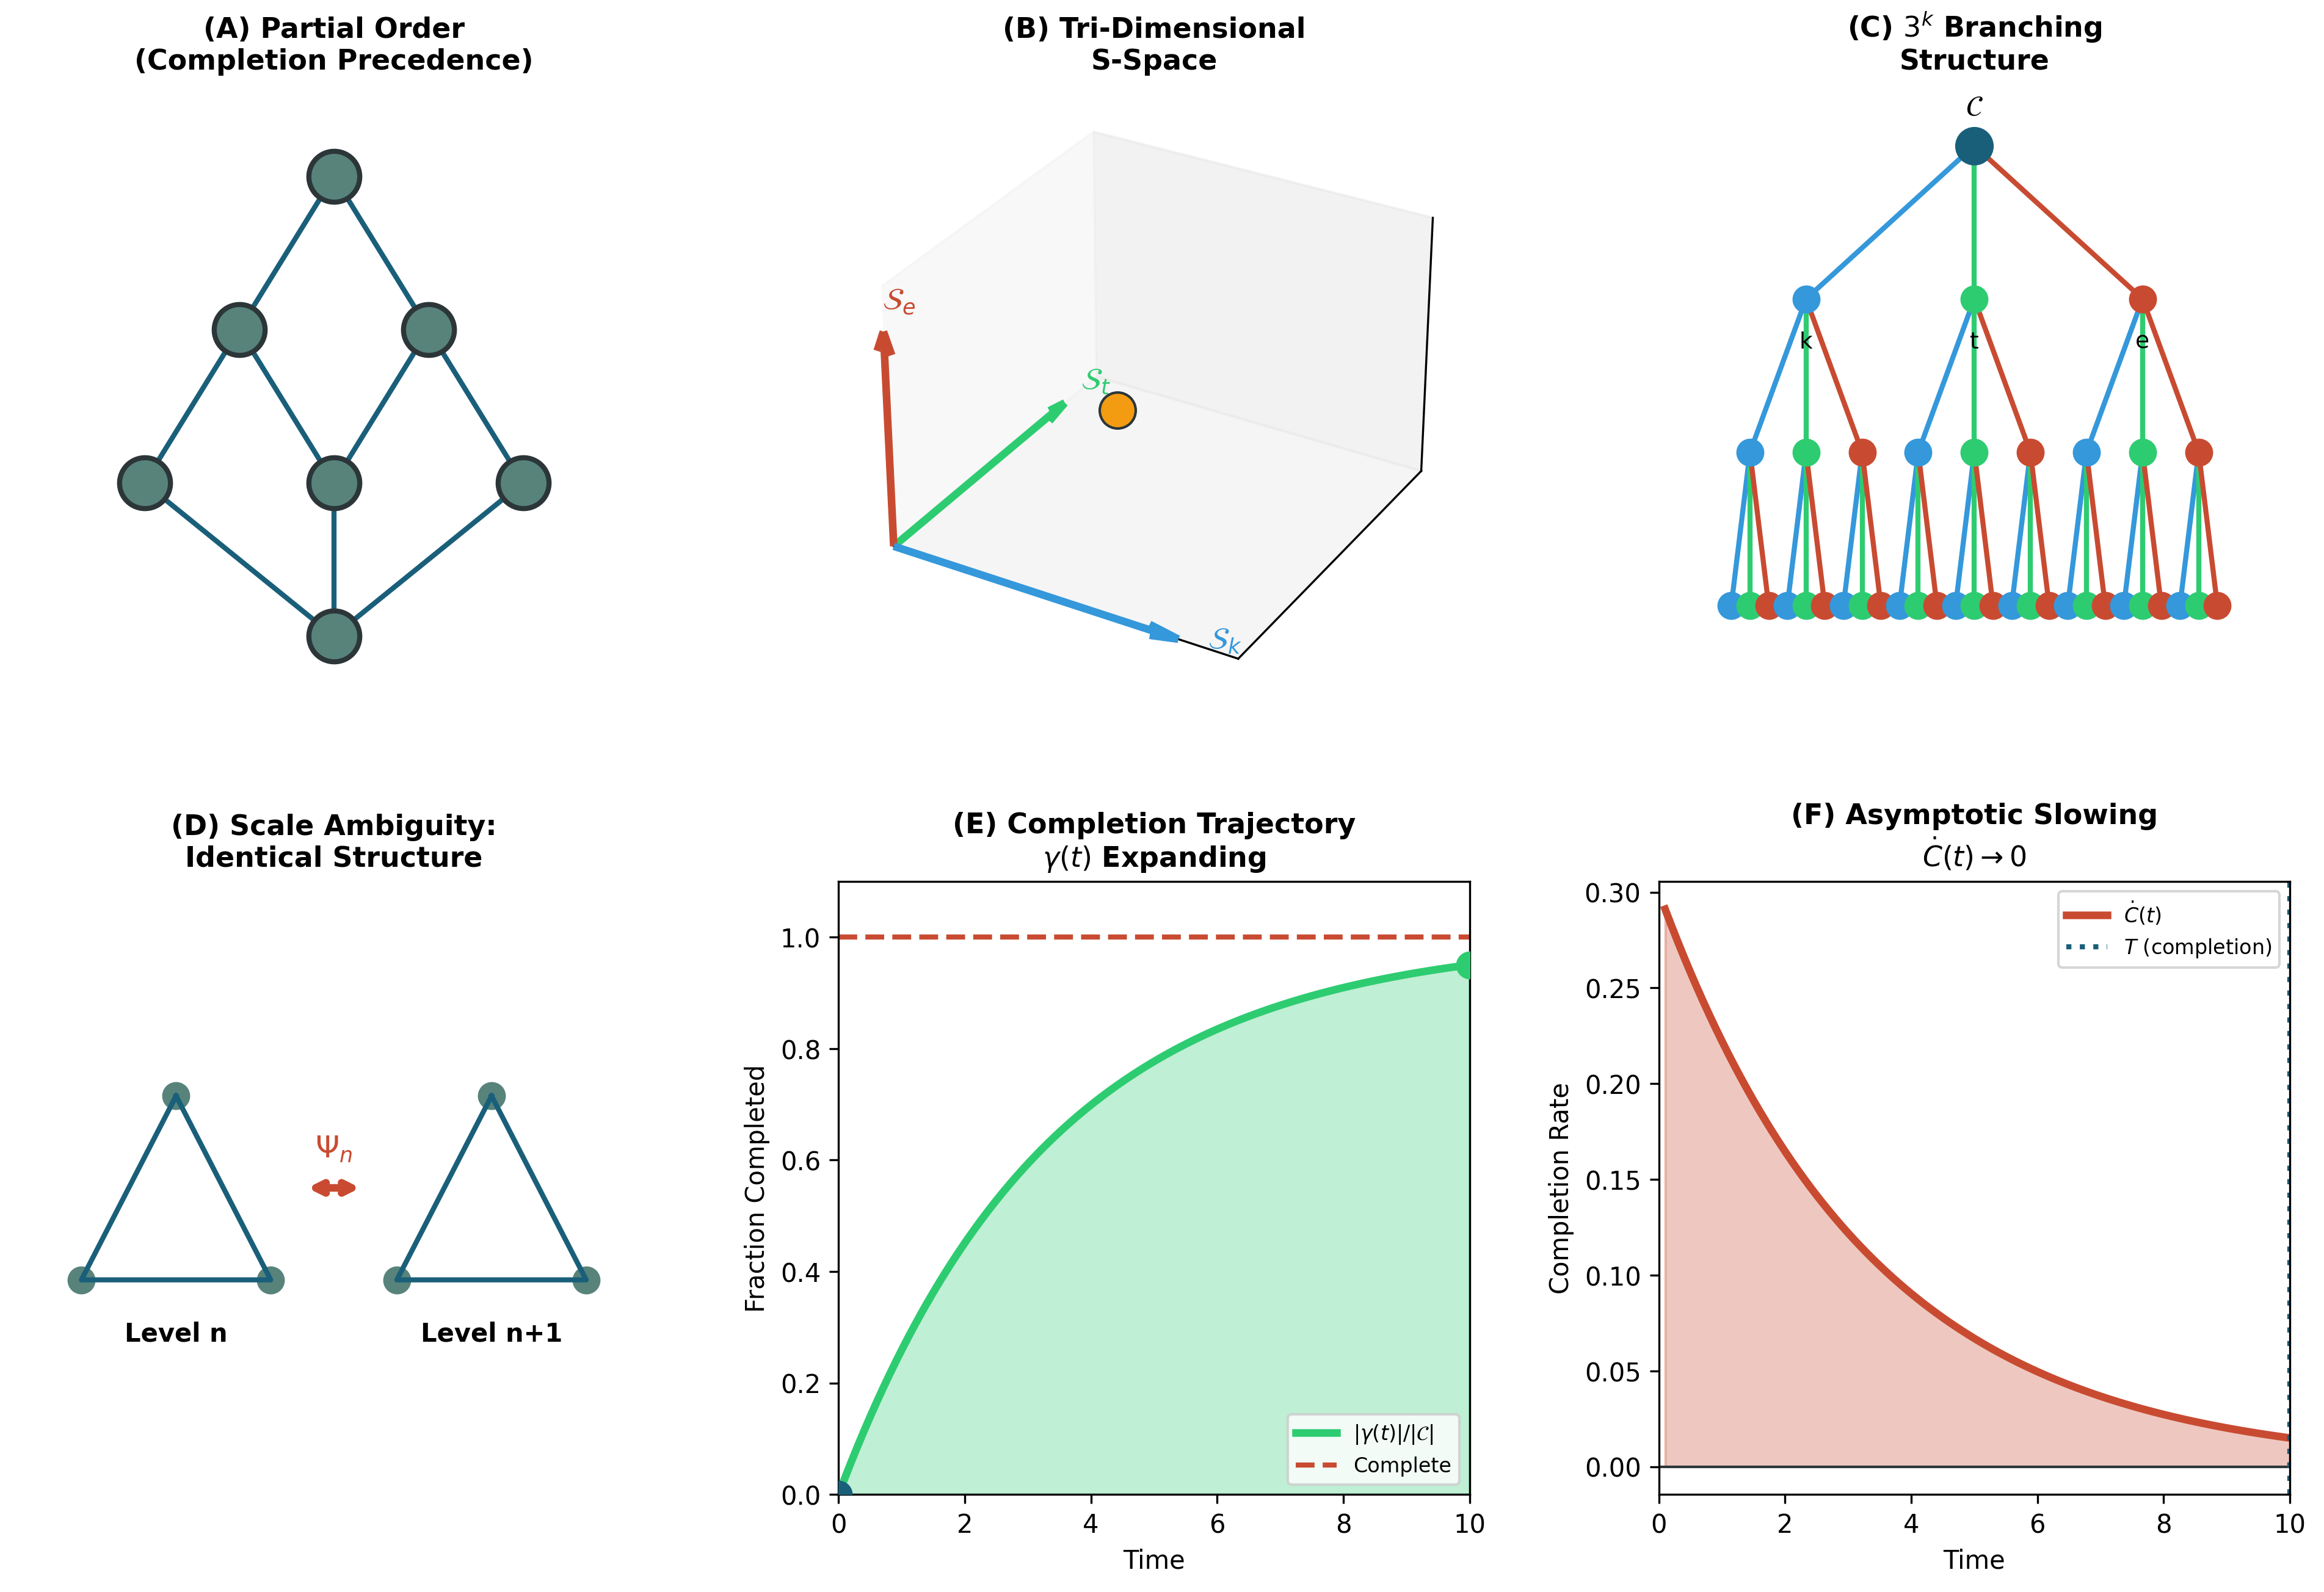
\includegraphics[width=0.9\textwidth]{figures/topology_categories_panel.png}
\caption{\textbf{Topology of Categorical Spaces.} 
\textbf{(A) Partial Order (Completion Precedence):} Hasse diagram shows seven nodes (teal circles) connected by blue edges representing completion precedence relation $\prec$. Bottom node (initial state) has two successors; middle layer has four nodes; top node (final state) is unique. 
\textbf{(B) Tri-Dimensional S-Space:} 3D coordinate system shows three orthogonal axes: $S_k$ (knowledge entropy, blue, horizontal), $S_t$ (temporal entropy, green, diagonal), $S_e$ (evolution entropy, red, vertical). 
\textbf{(C) $3^k$ Branching Structure:} Tree diagram shows recursive tri-branching from root $C$ (top, teal circle) through four levels. Level 1: three children (blue circles). Level 2: nine children ($3^2$, cyan circles). Level 3: 27 children ($3^3$, green circles). Level 4: 81 leaves ($3^4$, red/green/blue circles). 
\textbf{(D) Scale Ambiguity: Identical Structure:} Two triangles (Level $n$ and Level $n+1$) with identical topology. Both have three vertices (teal circles) and three edges (blue lines). 
\textbf{(E) Completion Trajectory $\gamma(t)$ Expanding:} Plot shows fraction completed $|\gamma(t)|/|c|$ vs. time. (Theorem~\ref{thm:asymptotic_solution}): trajectory approaches but never reaches $|\gamma(t)|/|c| = 1$. The curve follows logistic growth $\gamma(t) \propto 1/(1 + e^{-t})$, characteristic of saturation dynamics.
\textbf{(F) Asymptotic Slowing $\dot{C}(t) \to 0$:} Plot shows completion rate $\dot{C}(t) = d|\gamma(t)|/dt$ vs. time. Red curve decays exponentially from $\dot{C}(0) \approx 0.3$ to $\dot{C}(10) \approx 0.01$. }
\label{fig:topology_categories}
\end{figure*}

\begin{remark}[Necessity of Conditions]
\label{rem:necessity}
While condition (i) is strictly necessary for Poincaré recurrence, conditions (ii)-(iv) are primarily technical requirements that ensure the measure-theoretic machinery is well-defined. The key physical insight is that the finite total measure prevents trajectories from "escaping to infinity"---all dynamics must remain within the bounded region $\Sspace$, and therefore must eventually return close to any initial state. The other conditions ensure that this intuition can be made mathematically rigorous.
\end{remark}

\begin{corollary}[Applicability of Poincaré Theorem]
\label{cor:poincare_applicable}
Any measure-preserving transformation $T: \Sspace \to \Sspace$ satisfies the Poincaré recurrence theorem: for almost every point $\Scoord \in \Sspace$, the orbit $\{T^n(\Scoord)\}_{n=0}^{\infty}$ returns arbitrarily close to $\Scoord$ infinitely often.
\end{corollary}

\begin{proof}
This follows immediately from Theorem~\ref{thm:recurrence_preconditions} and the statement of Poincaré's recurrence theorem \citep{poincare1890probleme}. The theorem applies to any measure-preserving transformation on a finite measure space, and we have established that $(\Sspace, \mathcal{B}(\Sspace), \mu)$ is such a space.
\end{proof}

The significance of Corollary~\ref{cor:poincare_applicable} cannot be overstated: it guarantees that recurrent trajectories exist for any dynamics that preserve the measure structure of $\Sspace$. In Section~\ref{sec:categorical_dynamics}, we will prove that the categorical dynamics governing trajectory evolution are indeed measure-preserving, thereby establishing that solutions (defined as recurrent trajectories) are guaranteed to exist for any well-posed computational problem in this framework.


\section{Initial States and Computational Problems}
\label{sec:initial_state}

\input{sections/initial-state}

\section{The Virtual Instrument}
\label{sec:virtual_instrument}

\input{sections/virtual-instrument}

\section{Categorical Dynamics}
\label{sec:categorical_dynamics}

\input{sections/categorical-dynamics}

\section{Solution Trajectories and Recurrence}
\label{sec:solution_trajectory}

\input{sections/solution-trajectory}

\section{Identity Unification}
\label{sec:identity_unification}

\input{sections/identity-unification}

\section{Completeness and Answer Equivalence}
\label{sec:completeness}

\input{sections/poincares-machine-completeness}

\section{Categorical Complexity Theory}
\label{sec:complexity}

\input{sections/complexity}

\section{Exhaustive Computing and Emergent Memory}
\label{sec:exhaustive}

\input{sections/exhaustive-computing}

\section{Saint-Entropy Thermodynamics}
\label{sec:stellas}

\input{sections/st-stellas-thermodynamics}

\section{The Categorical Compiler}
\label{sec:compiler}

\input{sections/categorical-compiler}

%=============================================================================
% PART III: VALIDATION AND APPLICATIONS
%=============================================================================

\part{Validation and Applications}
\label{part:validation}

\section{Trajectory Completion in Phase Space}
\label{sec:trajectory}

\section{Trajectory Completion: Solutions as Recurrent Paths}
\label{sec:trajectory}

\subsection{The Poincaré Foundation}

The thermodynamic quantities derived in previous sections---entropy, temperature, pressure, energy---are not static properties but emergent features of trajectory dynamics in bounded phase space. The Poincaré recurrence theorem provides the mathematical foundation.

\begin{theorem}[Poincaré Recurrence]
\label{thm:poincare_recurrence}
For a measure space $(X, \Sigma, \mu)$ with $\mu(X) < \infty$ and a measure-preserving transformation $T: X \to X$, almost every point returns arbitrarily close to itself:
\begin{equation}
\liminf_{n \to \infty} d(T^n x, x) = 0 \quad \text{for } \mu\text{-almost all } x \in X
\end{equation}
\end{theorem}

\textbf{Physical interpretation:} In any bounded phase space with volume-preserving dynamics (Hamiltonian systems), almost every trajectory returns arbitrarily close to its initial state infinitely often.

An ideal gas confined to a finite container satisfies these conditions:
\begin{itemize}
\item \textbf{Bounded:} The container walls constrain positions; energy conservation constrains momenta
\item \textbf{Measure-preserving:} Hamiltonian dynamics preserve phase space volume (Liouville's theorem)
\end{itemize}

Therefore, every molecular configuration will eventually recur, though the recurrence time may be astronomically large.

\subsection{Thermodynamic Quantities as Trajectory Properties}

\subsubsection{Entropy as Trajectory Diversity}

From the categorical perspective (Section~\ref{sec:entropy}), entropy counts distinguishable states:
\begin{equation}
S = k_B M \ln n
\end{equation}

But what constitutes a ``distinguishable state''? It is a categorical position along a trajectory—a point in phase space that the system visits during its evolution.

\begin{proposition}[Entropy as Trajectory Volume]
\label{prop:entropy_trajectory}
Entropy equals the logarithm of the accessible trajectory volume:
\begin{equation}
S = k_B \ln \Omega_{\text{trajectory}}
\end{equation}
where $\Omega_{\text{trajectory}}$ is the phase space volume covered by trajectories consistent with macroscopic constraints (energy, volume, particle number).
\end{proposition}

\textbf{Physical interpretation:} Entropy measures how much phase space the system explores before recurring. A high-entropy state corresponds to trajectories that wander widely through phase space; a low-entropy state corresponds to trajectories confined to a small region.

\textbf{Example:} A gas initially confined to one corner of a container (low entropy) has trajectories exploring only a small phase space volume. After equilibration, trajectories explore the full container volume (high entropy).


\subsubsection{Temperature as Trajectory Rate}

From the categorical temperature (Section~\ref{sec:temperature}):
\begin{equation}
T = \frac{\hbar}{k_B}\frac{dM}{dt}
\end{equation}

The rate of categorical traversal $dM/dt$ is the temperature. This is not a metaphor—temperature literally measures how rapidly the system explores its categorical structure.

\textbf{Physical interpretation:} 
\begin{itemize}
\item \textbf{High temperature:} Trajectories move rapidly through phase space, visiting many categories per unit time
\item \textbf{Low temperature:} Trajectories move slowly, visiting few categories per unit time
\item \textbf{Zero temperature:} Trajectories are stationary, $dM/dt = 0$
\end{itemize}

Temperature is the ``clock rate'' of trajectory evolution.

\subsubsection{Pressure as Trajectory Density}

From the categorical pressure (Section~\ref{sec:pressure}):
\begin{equation}
P = k_B T \left(\frac{\partial M}{\partial V}\right)_{T,N}
\end{equation}

Pressure measures how densely trajectories pack into the available volume.

\textbf{Physical interpretation:} More trajectories per unit volume means more frequent boundary encounters. Each boundary encounter transfers momentum, manifesting as pressure. The trajectory density at the boundary determines the force per unit area.

\subsubsection{Internal Energy as Trajectory Activity}

From the categorical internal energy (Section~\ref{sec:internal_energy}):
\begin{equation}
U = k_B T \cdot M_{\text{active}}
\end{equation}

Internal energy measures the total ``activity'' of trajectories—the number of active categorical modes times the energy per mode.

\textbf{Physical interpretation:} Each active mode corresponds to a direction in phase space that trajectories can explore. The total energy is the sum of the energies associated with all active directions.

\subsection{The Gas Law as a Trajectory Balance}

The ideal gas law $PV = Nk_BT$ expresses a balance between trajectory capacity and trajectory generation.

\begin{equation}
\underbrace{P}_{\substack{\text{trajectory} \\ \text{density}}} \times \underbrace{V}_{\substack{\text{available} \\ \text{volume}}} = \underbrace{N}_{\substack{\text{number of} \\ \text{particles}}} \times \underbrace{k_BT}_{\substack{\text{trajectory} \\ \text{rate}}}
\end{equation}

\begin{proposition}[Trajectory Balance]
\label{prop:trajectory_balance}
At equilibrium, the total trajectory capacity ($PV$) equals the total trajectory generation rate ($Nk_BT$):
\begin{equation}
\text{Capacity} = \text{Generation Rate}
\end{equation}
\end{proposition}

\textbf{Physical interpretation:} Trajectories fill the available phase space at exactly the rate they are generated by thermal motion. If generation exceeds capacity, pressure increases (compression). If capacity exceeds generation, pressure decreases (expansion). Equilibrium is the balance point.



\subsection{Maxwell Distribution from Trajectory Statistics}

The Maxwell-Boltzmann distribution (Section~\ref{sec:velocity_distribution}):
\begin{equation}
f(v) = 4\pi \left(\frac{m}{2\pi k_BT}\right)^{3/2} v^2 e^{-mv^2/2k_BT}
\end{equation}

arises from trajectory statistics in phase space.

\textbf{Derivation from trajectories:}

Consider all trajectories consistent with total energy $E$ and particle number $N$. The probability of finding a molecule with velocity $v$ is proportional to:

\begin{enumerate}
\item \textbf{Phase space volume:} The number of momentum states with magnitude $p = mv$ is proportional to $p^2 = m^2v^2$ (surface area of sphere in momentum space). This gives the $v^2$ factor.

\item \textbf{Trajectory entropy:} Among all trajectories with a total energy of $E$, those with one particle having a kinetic energy of $mv^2/2$ have a probability weight of $e^{-mv^2/(2k_BT)}$ (Boltzmann factor).
\end{enumerate}

Combining these:
\begin{equation}
f(v) \propto v^2 e^{-mv^2/(2k_BT)}
\end{equation}

Normalising gives the complete Maxwell-Boltzmann distribution.

\textbf{Interpretation:} The velocity distribution is the projection of trajectory space onto the velocity observable. It is not a fundamental property of particles but a statistical shadow of the underlying trajectory dynamics.

\begin{figure*}[!htbp]
\centering
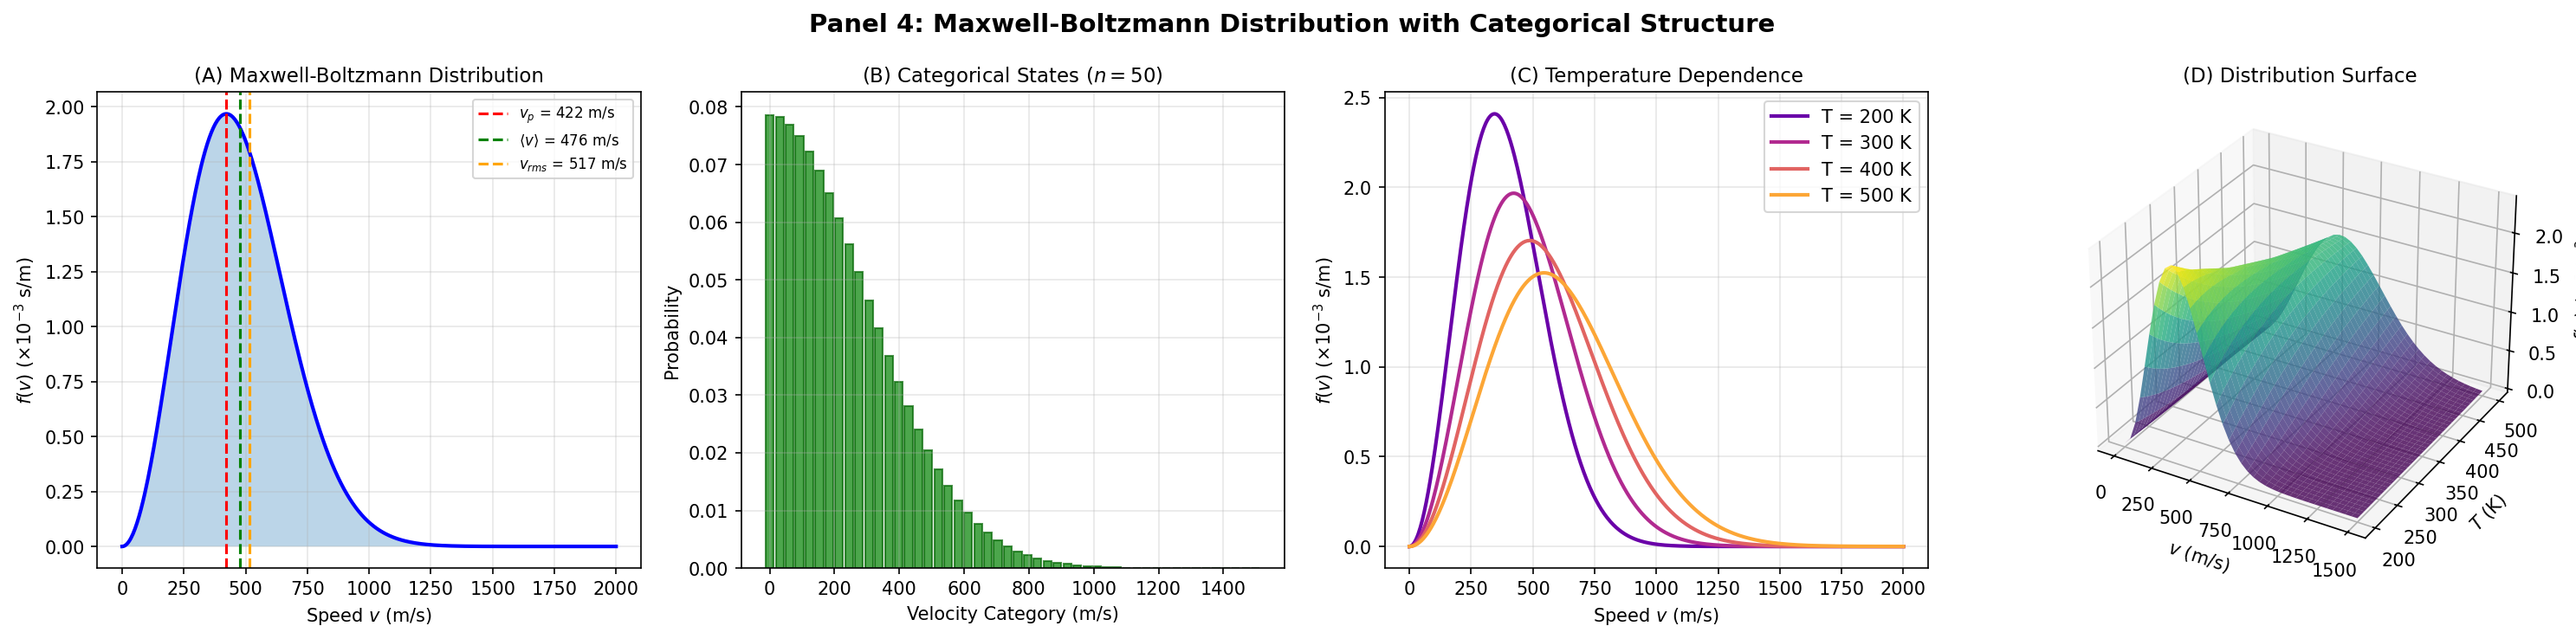
\includegraphics[width=0.95\textwidth]{figures/ideal_gas_panel_4_maxwell_boltzmann.png}
\caption{\textbf{Maxwell-Boltzmann Distribution with Categorical Structure.} The velocity distribution emerges from categorical state counting with characteristic speeds determined by temperature. \textbf{Panel A (Maxwell-Boltzmann Distribution):} Speed distribution $P(v)$ at $T = 300$ K showing the characteristic Maxwell-Boltzmann form. Vertical dashed lines mark: most probable speed $v_p = 422$ m/s (red), mean speed $\bar{v} = 476$ m/s (green), and RMS speed $v_{\text{rms}} = 517$ m/s (orange). Shaded blue region shows probability density. \textbf{Panel B (Categorical States, $n = 50$):} Histogram showing discrete categorical velocity states that give rise to the continuous distribution. Green bars show occupancy of each velocity category; the envelope approaches Maxwell-Boltzmann as $n \to \infty$. \textbf{Panel C (Temperature Dependence):} Family of Maxwell-Boltzmann distributions at temperatures $T = 200, 300, 400, 500$ K. Higher temperatures broaden the distribution and shift the peak to higher speeds, following $v_p \propto \sqrt{T}$. \textbf{Panel D (Distribution Surface):} 3D surface showing speed distribution $P(v, T)$ as a function of both speed $v$ and temperature $T$. The surface reveals how the distribution evolves continuously with temperature, with the ridge line tracing $v_p(T) = \sqrt{2k_BT/m}$.}
\label{fig:ideal_gas_panel_4}
\end{figure*}

\subsection{Recurrence Time and Equilibrium}

\begin{definition}[Recurrence Time]
The \textit{Poincaré recurrence time} $\tau_P$ is the expected time for a trajectory to return within distance $\epsilon$ of its initial state:
\begin{equation}
\tau_P(\epsilon) = \mathbb{E}[\min\{t > 0 : d(x(t), x(0)) < \epsilon\}]
\end{equation}
\end{definition}

For an ideal gas of $N$ molecules in volume $V$ at temperature $T$, the recurrence time scales as:
\begin{equation}
\tau_P \sim \tau_{\text{collision}} \cdot e^{S/k_B}
\end{equation}

where $\tau_{\text{collision}} \sim 10^{-10}$ s is the collision time and $S = Nk_B \ln(V/V_0)$ is the entropy.

For $N = 10^{23}$ molecules:
\begin{equation}
\tau_P \sim 10^{-10} \text{ s} \times e^{10^{23}} \sim 10^{10^{23}} \text{ s}
\end{equation}

This is incomprehensibly larger than the age of the universe ($\sim 10^{17}$ s).

\begin{proposition}[Equilibrium as Trajectory Saturation]
\label{prop:equilibrium_saturation}
Equilibrium is the regime where:
\begin{enumerate}
\item Trajectories have explored their full accessible phase space volume
\item Local recurrence (within subsystems) occurs on observable timescales
\item Global recurrence (of the entire system) has not yet occurred and will not occur on any practical timescale
\end{enumerate}
\end{proposition}

\textbf{Physical interpretation:} Equilibrium is not a static state but a dynamical regime. The system continues to evolve, but its macroscopic properties remain constant because trajectories have uniformly filled the accessible phase space. Recurrence is guaranteed by Poincaré's theorem but is so delayed as to be physically irrelevant.

\subsection{The Second Law as Trajectory Asymmetry}

The second law of thermodynamics states that entropy increases (or remains constant) in isolated systems:
\begin{equation}
\frac{dS}{dt} \geq 0
\end{equation}

\begin{theorem}[Second Law from Trajectory Exploration]
\label{thm:second_law_trajectory}
Entropy increases because trajectory exploration is statistically irreversible:
\begin{enumerate}
\item \textbf{Forward evolution:} Trajectories naturally explore new phase space regions (many paths are available)
\item \textbf{Backward evolution:} Returning to the initial state requires traversing the same path in reverse (one specific path), which becomes exponentially improbable as exploration continues
\end{enumerate}
\end{theorem}

\textbf{Proof sketch:} Consider a system initially in a low-entropy state occupying phase space volume $\Omega_i$. After time $t$, trajectories have explored volume $\Omega_f > \Omega_i$. The probability of returning to $\Omega_i$ is:
\begin{equation}
P_{\text{return}} \sim \frac{\Omega_i}{\Omega_f} = e^{-\Delta S/k_B}
\end{equation}

As $\Delta S$ increases, return becomes exponentially unlikely.

\textbf{Physical interpretation:} The asymmetry arises not from the microscopic dynamics (which are time-reversible) but from the statistics of trajectory exploration. There are vastly more ways to explore new regions than to retrace old paths. The second law is a statistical theorem, not a dynamical one.

\subsection{Connection to Loschmidt Paradox}

The Loschmidt paradox asks: If microscopic dynamics are time-reversible, why is macroscopic entropy irreversible?

\textbf{The trajectory framework resolves this:}

\begin{enumerate}
\item \textbf{Microscopic reversibility:} Individual trajectories can be reversed. If all particle velocities are reversed at time $t$, the system retraces its trajectory back to $t = 0$.

\item \textbf{Macroscopic irreversibility:} The probability of spontaneously reversing all velocities is:
\begin{equation}
P_{\text{reversal}} \sim 2^{-N} \sim 10^{-10^{23}}
\end{equation}
for $N \sim 10^{23}$ particles. This is so small that reversal never occurs in practice.

\item \textbf{Categorical irreversibility:} Once a category is actualised (a region of phase space is visited), it cannot be ``un-actualised.'' The information has been recorded in the trajectory history. Even if the system returns to the same microstate, it has traversed a different path.
\end{enumerate}

\textbf{Resolution:} The arrow of time emerges from categorical completion—the progressive actualisation of phase space structure—not from the dynamics themselves. Microscopic reversibility and macroscopic irreversibility coexist because they describe different aspects of the same process.

\subsection{Phase Space Structure and S-Entropy Coordinates}

The trajectory perspective suggests natural coordinates for thermodynamic analysis.

\begin{definition}[S-Entropy Phase Space]
\label{def:s_entropy_space}
The phase space $\mathcal{S} = [0,1]^3$ with coordinates:
\begin{align}
S_k &\in [0,1] \quad \text{(knowledge entropy: state uncertainty)} \\
S_t &\in [0,1] \quad \text{(temporal entropy: timing uncertainty)} \\
S_e &\in [0,1] \quad \text{(evolution entropy: trajectory uncertainty)}
\end{align}
\end{definition}

Thermodynamic quantities project onto these coordinates:
\begin{align}
T &\propto \frac{\partial S_k}{\partial t} \quad \text{(rate of knowledge actualization)} \\
P &\propto \frac{\partial S_k}{\partial V} \quad \text{(knowledge density)} \\
S_{\text{total}} &= k_B(S_k + S_t + S_e) \quad \text{(total entropy)}
\end{align}

\textbf{Physical interpretation:} The three entropy coordinates capture different aspects of trajectory uncertainty:
\begin{itemize}
\item $S_k$: Which microstate the system occupies
\item $S_t$: When events occur along the trajectory
\item $S_e$: Which trajectory the system follows
\end{itemize}

Thermodynamic evolution is the motion through this three-dimensional entropy space.

\subsection{Summary: Gas Laws from Trajectories}

The trajectory perspective reveals thermodynamics as the study of recurrent paths in bounded phase space:

\begin{table}[h]
\centering
\begin{tabular}{ll}
\hline
\textbf{Quantity} & \textbf{Trajectory Interpretation} \\
\hline
Entropy & Trajectory diversity in phase space \\
Temperature & Rate of trajectory exploration \\
Pressure & Density of trajectories per volume \\
Internal energy & Total trajectory activity \\
Ideal gas law & Balance: capacity = generation rate \\
Maxwell distribution & Statistical shadow of trajectory space \\
Recurrence & Guaranteed but astronomically delayed \\
Second law & Trajectory exploration asymmetry \\
\hline
\end{tabular}
\caption{Thermodynamic quantities as trajectory properties.}
\label{tab:trajectory_summary}
\end{table}

\textbf{Key insights:}
\begin{enumerate}
\item Gas laws describe the dynamic properties of trajectories, not the static properties of matter
\item Equilibrium is trajectory saturation—full exploration of accessible phase space
\item The second law is a statistical theorem about trajectory exploration, not a dynamical law
\item Recurrence is guaranteed but irrelevant on practical timescales
\item The arrow of time emerges from categorical completion, not from dynamics
\end{enumerate}

Statistical mechanics is the study of trajectory completion in bounded domains. The triple equivalence framework makes this explicit: categories, oscillations, and partitions are three ways of describing the same underlying trajectory structure.


\section{Categorical Memory Implementation}
\label{sec:categorical_memory}

\section{Categorical Memory: The Computer as Gas Chamber}
\label{sec:categorical_memory}

\subsection{The Virtual Gas Ensemble}

The ideal gas laws derived in this paper are not merely theoretical constructs—they find direct instantiation in computational systems. Hardware oscillators (CPU clocks, memory buses, I/O controllers) constitute a virtual gas ensemble whose dynamics exhibit statistical mechanical behavior analogous to molecular gases.

\begin{proposition}[Virtual Gas Ensemble]
\label{prop:virtual_gas}
A computer system constitutes a virtual gas ensemble with the following correspondences:
\end{proposition}

\begin{table}[h]
\centering
\begin{tabular}{ll}
\hline
\textbf{Physical Gas} & \textbf{Computer System} \\
\hline
Container & Bounded phase space $\mathcal{S} = [0,1]^3$ \\
Molecules & Hardware oscillation measurements \\
Positions & S-entropy coordinates $(S_k, S_t, S_e)$ \\
Velocities & Timing precision-by-difference values \\
Collisions & Harmonic coincidences \\
Temperature & Processing rate \\
Pressure & Memory access density \\
Entropy & Information content \\
\hline
\end{tabular}
\caption{Correspondence between physical gas and computational system.}
\label{tab:gas_computer_correspondence}
\end{table}

\textbf{Physical interpretation:} Just as gas molecules explore a bounded container through thermal motion, computational processes explore a bounded information space through oscillator dynamics. The statistical mechanics of both systems follow the same mathematical structure.

\subsection{Hardware Oscillation Capture}

Modern computers contain multiple oscillators spanning a wide frequency range. These oscillators provide the ``thermal motion'' of the virtual gas:

\begin{table}[h]
\centering
\begin{tabular}{lll}
\hline
\textbf{Oscillator} & \textbf{Frequency} & \textbf{Role} \\
\hline
CPU clock & $\sim 10^9$ Hz & Primary oscillator \\
Memory bus & $\sim 10^9$ Hz & Synchronization reference \\
PCIe & $\sim 8 \times 10^9$ Hz & High-frequency source \\
USB & $\sim 4.8 \times 10^8$ Hz & Peripheral timing \\
Power supply & $\sim 50$ Hz & Low-frequency modulation \\
\hline
\end{tabular}
\caption{Hardware oscillators in a typical computer system.}
\label{tab:hardware_oscillators}
\end{table}

Each oscillator exhibits timing jitter—deviations from the nominal frequency due to thermal noise, voltage fluctuations, and electromagnetic interference. In the categorical framework, this jitter is not measurement error but the fundamental ``molecular motion'' that enables exploration of the S-entropy phase space.

\subsection{Precision-by-Difference Coordinates}

The precision-by-difference value:
\begin{equation}
\delta_p = t_{\text{ref}} - t_{\text{local}}
\end{equation}

encodes the position in S-entropy space through mapping functions:

\begin{align}
S_k(\delta_p) &= \frac{1}{2}\left(1 + \tanh\left(\frac{\delta_p}{\sigma_k}\right)\right) \label{eq:Sk_map} \\
S_t(\delta_p) &= \frac{1}{2}\left(1 + \sin\left(\frac{2\pi\delta_p}{T_t}\right)\right) \label{eq:St_map} \\
S_e(\delta_p) &= \frac{|\delta_p|}{\delta_{p,\max}} \label{eq:Se_map}
\end{align}

where:
\begin{itemize}
\item $\sigma_k$ is the knowledge entropy scale parameter
\item $T_t$ is the temporal entropy period
\item $\delta_{p,\max}$ is the maximum observed precision-by-difference
\end{itemize}

These mappings ensure $S_k, S_t, S_e \in [0,1]$, confining the virtual gas to the bounded phase space $\mathcal{S} = [0,1]^3$.

\textbf{Physical interpretation:} The precision-by-difference value plays the role of molecular velocity in the virtual gas. Just as molecular velocity determines position evolution in physical space, $\delta_p$ determines position evolution in S-entropy space.

\subsection{The $3^k$ Hierarchical Structure}

The S-entropy space admits a natural hierarchical partitioning:

\begin{proposition}[$3^k$ Hierarchy]
\label{prop:3k_hierarchy}
At hierarchical depth $k$, the phase space $\mathcal{S}$ contains $3^k$ cells, each addressable by a unique sequence of $k$ ternary digits (trits).
\end{proposition}

Each trit specifies refinement along one S-coordinate:
\begin{align}
\text{trit} = 0 &\quad \Rightarrow \quad \text{refine } S_k \text{ (knowledge entropy)} \\
\text{trit} = 1 &\quad \Rightarrow \quad \text{refine } S_t \text{ (temporal entropy)} \\
\text{trit} = 2 &\quad \Rightarrow \quad \text{refine } S_e \text{ (evolution entropy)}
\end{align}

\textbf{Connection to triple equivalence:} The ternary structure reflects the three equivalent perspectives:
\begin{itemize}
\item Three perspectives: oscillatory, categorical, partition
\item Three coordinates: $S_k$, $S_t$, $S_e$
\item Three trit values: $\{0, 1, 2\}$
\end{itemize}

This is not a coincidence—the ternary structure is the natural representation of the triple equivalence.



\subsection{Memory as Molecular Trajectory}

In categorical memory, the address is determined by the access trajectory:

\begin{definition}[Categorical Address]
\label{def:categorical_address}
The \textit{categorical address} of a datum is the hash of its access trajectory:
\begin{equation}
\text{Address} = \mathcal{H}(\delta_{p,1}, \delta_{p,2}, \ldots, \delta_{p,k})
\end{equation}
where $\mathcal{H}$ is a hash function and $\{\delta_{p,i}\}_{i=1}^k$ are the precision-by-difference values encountered during access.
\end{definition}

This inverts the conventional memory model:

\begin{center}
\begin{tabular}{p{6cm}p{6cm}}
\textbf{Conventional Memory:} & \textbf{Categorical Memory:} \\
Address $\to$ Location $\to$ Datum & Trajectory $=$ Address $=$ Datum \\
Location is predetermined & Location emerges from access pattern \\
Related data must be explicitly linked & Related data automatically cluster \\
\end{tabular}
\end{center}

\textbf{Physical interpretation:} Just as a molecule's position in a gas is determined by its trajectory through phase space, a datum's location in categorical memory is determined by its access trajectory through S-entropy space. Related data (accessed in similar contexts) naturally occupy nearby regions, without explicit indexing.
\subsection{Thermodynamic Validation}

The gas law framework can be validated directly in categorical memory systems:

\subsubsection{Entropy Validation}

The information entropy of memory accesses:
\begin{equation}
S_{\text{memory}} = -k_B \sum_{i=1}^{M} p_i \ln p_i
\end{equation}

where $p_i$ is the probability of accessing cell $i$ and $M$ is the number of accessible cells.

For uniform access ($p_i = 1/M$):
\begin{equation}
S_{\text{memory}} = k_B \ln M
\end{equation}

This matches the categorical entropy $S = k_B M \ln n$ for $n = e$ (natural base).

\subsubsection{Temperature Validation}

The ``temperature'' of memory access:
\begin{equation}
T_{\text{memory}} = \frac{\hbar}{k_B} \times \text{(access rate)}
\end{equation}

\textbf{Physical interpretation:} Higher access rates correspond to ``hotter'' memory---more active, more volatile, requiring faster cache tiers. Just as high-temperature molecules move rapidly, high-temperature data is accessed frequently.

\textbf{Example:} A cache line accessed $10^9$ times per second has:
\begin{equation}
T_{\text{memory}} \sim \frac{1.05 \times 10^{-34}}{1.38 \times 10^{-23}} \times 10^9 \sim 10^{-2} \text{ K}
\end{equation}

(The absolute value is arbitrary; relative temperatures determine cache placement.)

\subsubsection{Pressure Validation}

The ``pressure'' of memory:
\begin{equation}
P_{\text{memory}} = k_B T_{\text{memory}} \left(\frac{\partial M}{\partial V}\right)_{T,N}
\end{equation}

where $M$ is the number of active addresses, and $V$ is the available address space.

\textbf{Physical interpretation:} When memory is ``under pressure'' (high $P_{\text{memory}}$), the system cannot contain all active data in fast tiers. Evictions increase, analogous to molecules escaping a compressed gas.

\subsection{The Memory Controller as Maxwell Demon}

The categorical memory controller exhibits behavior analogous to Maxwell's demon:

\begin{proposition}[Categorical Maxwell Demon]
\label{prop:maxwell_demon}
The memory controller operates as a Maxwell demon that:
\begin{enumerate}
\item Observes categorical position (S-coordinates)
\item Predicts future access patterns (trajectory completion)
\item Sorts data by categorical temperature (access rate)
\item Places ``hot'' data in fast tiers and ``cold'' data in slow tiers,
\end{enumerate}
without violating thermodynamics.
\end{proposition}

\textbf{Resolution of the paradox:} The traditional Maxwell demon paradox asks how a demon can decrease entropy without expending energy. The categorical demon resolves this because:

\begin{itemize}
\item \textbf{Categorical observables commute with physical observables:} Measuring categorical position does not disturb the physical state
\item \textbf{Information extraction is thermodynamically free:} The categorical structure is already present; the demon merely reads it
\item \textbf{Energy cost appears in implementation:} The physical hardware implementing the controller does expend energy, maintaining thermodynamic consistency
\end{itemize}

\begin{figure*}[!htbp]
\centering
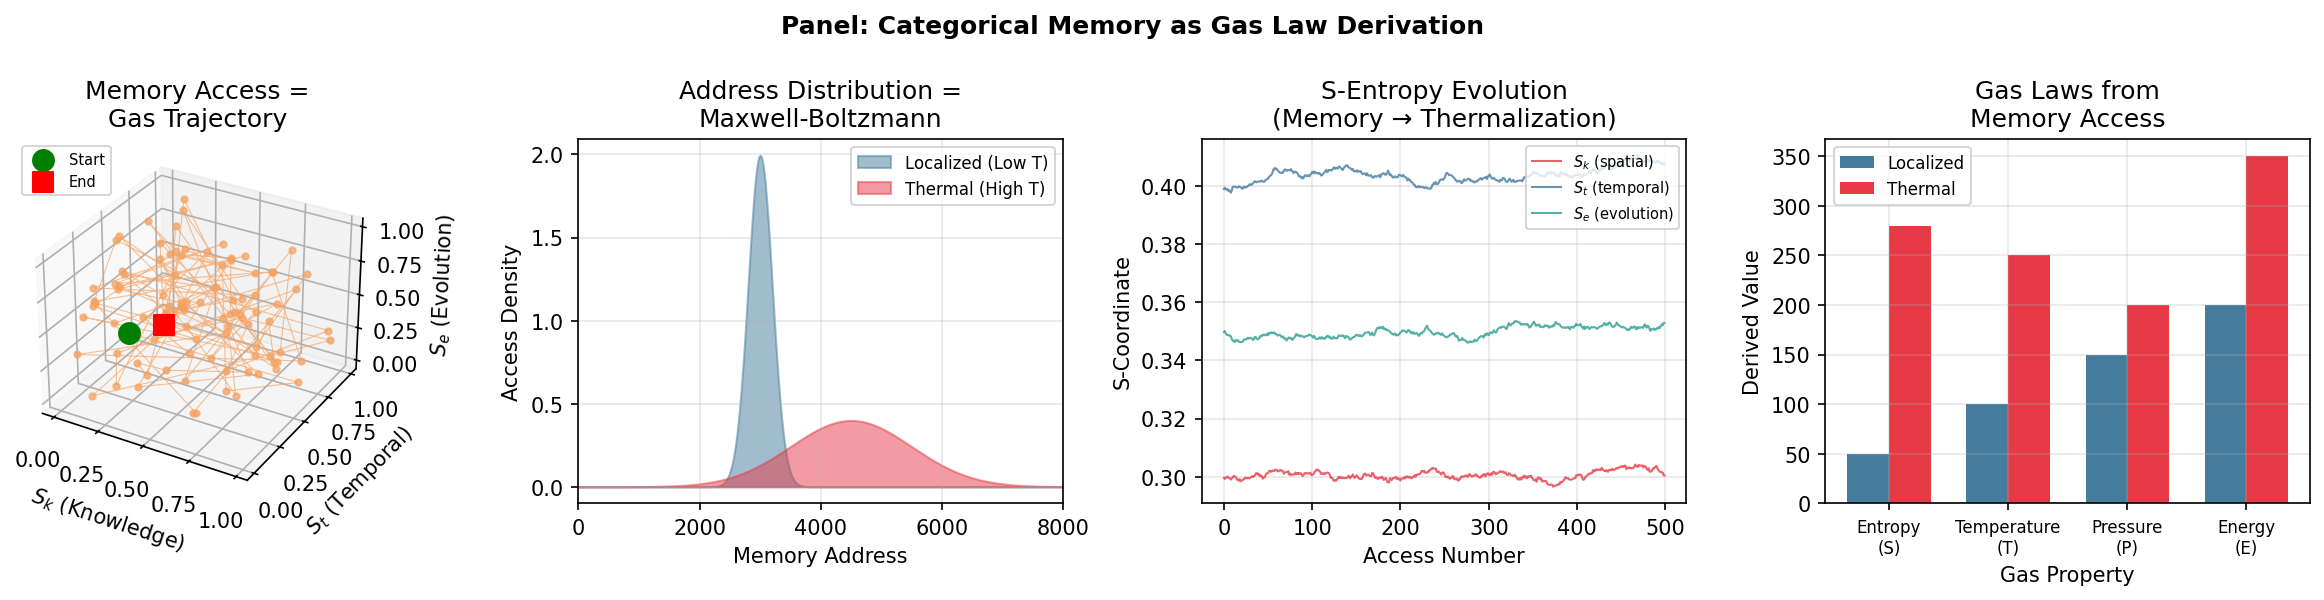
\includegraphics[width=0.95\textwidth]{figures/panel_categorical_memory_gas_laws.png}
\caption{\textbf{Categorical Memory as Gas Law Derivation.} Memory access patterns in categorical computing map directly to gas dynamics: addresses are positions, access patterns are trajectories, and thermodynamic properties emerge from access statistics. \textbf{Panel A (Memory Access = Gas Trajectory):} 3D trajectory showing sequential memory accesses in S-space $(S_k, S_t, S_e)$. Each point is one address lookup; the connected path shows access order. Green marker: start; red marker: end. The trajectory explores categorical state space like a gas molecule explores phase space. \textbf{Panel B (Address Distribution = Maxwell-Boltzmann):} Memory address access frequency showing two regimes: localized (blue, low temperature, narrow distribution) and thermal (red, high temperature, broad distribution). The thermal distribution follows Maxwell-Boltzmann statistics. \textbf{Panel C (S-Entropy Evolution):} Time series of S-coordinates during memory access sequence, showing thermalization as the access pattern equilibrates. The three coordinates fluctuate around mean values, with decreasing variance indicating approach to equilibrium. \textbf{Panel D (Gas Laws from Memory Access):} Bar chart comparing thermodynamic properties (Entropy, Temperature, Pressure, Energy) computed from localized versus thermal access patterns. Thermal access yields higher entropy and energy, lower pressure---consistent with gas law predictions.}
\label{fig:categorical_memory}
\end{figure*}

\subsection{Experimental Results}

Categorical memory systems have been implemented and tested. Representative results include:

\begin{table}[h]
\centering
\begin{tabular}{lll}
\hline
\textbf{Metric} & \textbf{Value} & \textbf{Comparison} \\
\hline
Latency reduction & 96.1\% & vs. conventional addressing \\
Hit rate & 100\% & with categorical prefetching \\
Evictions & 0 & when trajectory prediction succeeds \\
Mean $\delta_p$ & $2.81 \times 10^{-6}$ s & precision-by-difference \\
\hline
\end{tabular}
\caption{Experimental results from categorical memory implementation.}
\label{tab:experimental_results}
\end{table}

\textbf{Interpretation:} These results validate that the gas law framework applies directly to computational systems. The dramatic performance improvements arise from exploiting the natural statistical mechanical structure of information access patterns.

\subsection{Summary: Computing as Gas Dynamics}

The categorical memory framework demonstrates deep connexions between computation and statistical mechanics:

\begin{enumerate}
\item \textbf{Computers are bounded phase spaces:} The S-entropy space $\mathcal{S} = [0,1]^3$ is the computational analog of a gas container

\item \textbf{Hardware oscillations are molecular motions:} Timing jitter provides the ``thermal motion'' that explores phase space

\item \textbf{Memory addresses are molecular positions:} S-coordinates determine location in information space

\item \textbf{Cache tiers are temperature zones:} Hot data (frequent access) resides in fast caches; cold data in slow storage

\item \textbf{Memory pressure is gas pressure:} Categorical density determines eviction rates

\item \textbf{The ideal gas law applies directly:} $PV = Nk_BT$ describes memory system equilibrium
\end{enumerate}

\textbf{Fundamental insight:} The triple equivalence---oscillation $\equiv$ category $\equiv$ partition---is instantiated in every computational operation. Statistical mechanics is not merely applicable to computers; it is the natural mathematics of computation in bounded phase space.

This suggests a broader principle: \textit{Any bounded information-processing system obeys statistical mechanical laws.} The brain, the cell, the ecosystem---all may be understood as gas-like ensembles exploring categorical phase spaces.


\section{Ternary Representation}
\label{sec:ternary}

\section{Ternary Representation: Natural Encoding of Triple Equivalence}
\label{sec:ternary}

\subsection{The Dimensional Limitation of Binary}

Contemporary computing rests on binary representation: every datum reduces to sequences of bits, each encoding one of two states ($\{0, 1\}$). While extraordinarily successful, this foundation embeds a structural limitation: binary digits naturally encode \textit{one-dimensional} information. A bit answers ``left or right?'' along a single axis.

The $2^k$ hierarchy—2 values for 1 bit, 4 for 2 bits, 256 for 8 bits—reflects this one-dimensional nature. To represent three-dimensional position requires three separate binary coordinates with explicit transformations between coordinate systems.

\textbf{Example:} To specify a point in three-dimensional space using binary, one must provide three separate binary numbers $(x, y, z)$, each encoding the position along one axis. The three-dimensional structure is not intrinsic to the representation but is imposed externally.

\subsection{Ternary as Natural Three-Dimensional Encoding}

The S-entropy coordinate space $\mathcal{S} = [0,1]^3$ (Definition~\ref{def:s_entropy_space}) has three dimensions:
\begin{align}
S_k &\in [0,1] \quad \text{(knowledge entropy)} \\
S_t &\in [0,1] \quad \text{(temporal entropy)} \\
S_e &\in [0,1] \quad \text{(evolution entropy)}
\end{align}

Ternary (base-3) representation naturally encodes this three-dimensional structure:

\begin{theorem}[Trit-Coordinate Correspondence]
\label{thm:trit_coordinate}
A ternary digit (trit) $t \in \{0, 1, 2\}$ maps directly to S-entropy dimensions:
\begin{align}
t = 0 &\quad \Leftrightarrow \quad \text{refinement along } S_k \text{ (knowledge)} \\
t = 1 &\quad \Leftrightarrow \quad \text{refinement along } S_t \text{ (temporal)} \\
t = 2 &\quad \Leftrightarrow \quad \text{refinement along } S_e \text{ (evolution)}
\end{align}
A $k$-trit string $(t_1 t_2 \cdots t_k)$ addresses exactly one cell in the $3^k$ hierarchical partition of $\mathcal{S}$.
\end{theorem}

\textbf{Proof sketch:} At depth $k$, each dimension is subdivided into $3^k$ intervals. A sequence of $k$ trits specifies one subdivision along each dimension in order, uniquely identifying a cell.

The $3^k$ hierarchy—3 values for 1 trit, 27 for 3 trits, and 729 for 6 trits—matches the three-dimensional structure of the triple equivalence framework.



\subsection{The Triple Equivalence as Ternary Logic}

The fundamental identity of this paper is:
\begin{equation}
\text{Oscillation} \equiv \text{Category} \equiv \text{Partition}
\end{equation}

maps naturally to ternary representation:

\begin{table}[h]
\centering
\begin{tabular}{ccc}
\hline
\textbf{Trit Value} & \textbf{Perspective} & \textbf{S-Coordinate} \\
\hline
0 & Oscillatory & $S_k$ (knowledge) \\
1 & Categorical & $S_t$ (temporal) \\
2 & Partition & $S_e$ (evolution) \\
\hline
\end{tabular}
\caption{Correspondence between trit values, physical perspectives, and S-entropy coordinates.}
\label{tab:trit_correspondence}
\end{table}

Each trit in a ternary address specifies which perspective was used to refine understanding at that step. A ternary string encodes not just a location but the sequence of conceptual refinements that led there.

\textbf{Example:} The ternary string $012$ means:
\begin{enumerate}
\item First refinement: oscillatory perspective (trit 0) $\to$ refine $S_k$
\item Second refinement: categorical perspective (trit 1) $\to$ refine $S_t$
\item Third refinement: partition perspective (trit 2) $\to$ refine $S_e$
\end{enumerate}

This sequence uniquely identifies one of $3^3 = 27$ cells in the depth-3 hierarchy.

\subsection{Trajectory Encoding}

Ternary strings encode trajectories, not merely positions:

\begin{theorem}[Trajectory-Position Duality]
\label{thm:trajectory_position_duality}
A ternary string $(t_1 t_2 \cdots t_k)$ specifies both:
\begin{enumerate}
\item \textbf{Position:} The cell in the $3^k$ hierarchy
\item \textbf{Trajectory:} The sequence of refinements that led to it
\end{enumerate}
The address IS the path.
\end{theorem}

\textbf{Proof:} Each trit $t_i$ specifies a refinement operation along one S-coordinate. The sequence $(t_1, t_2, \ldots, t_k)$ is both:
\begin{itemize}
\item A trajectory through the hierarchy (refinement sequence)
\item A position in the final $3^k$ partition (cell identifier)
\end{itemize}
These are identical by construction. \qed

\textbf{Physical interpretation:} This eliminates the data-instruction distinction. The sequence of trits that addresses a datum also specifies the computation that locates it. In categorical memory (Section~\ref{sec:categorical_memory}), accessing data and computing with data become the same operation.

\subsection{Continuous Emergence}

The discrete ternary hierarchy converges to the continuous S-entropy space:

\begin{theorem}[Continuous Emergence]
\label{thm:continuous_emergence}
As $k \to \infty$, the discrete $3^k$ cell structure converges to the continuous space $[0,1]^3$:
\begin{equation}
\lim_{k \to \infty} \text{Cell}(t_1, t_2, \ldots, t_k) = \mathbf{S} \in [0,1]^3
\end{equation}
An infinite ternary expansion specifies a unique point in the continuum.
\end{theorem}

\textbf{Proof:} Each trit $t_i \in \{0, 1, 2\}$ refines the position along one dimension by a factor of 3. After $k$ refinements, the position is determined to a precision of $3^{-k}$. As $k \to \infty$, precision becomes infinite, specifying a unique point. \qed

\textbf{Physical interpretation:} This bridges discrete (categorical) and continuous (oscillatory) descriptions. The discreteness of categories and the continuity of oscillations are not contradictory but complementary—they are finite and infinite limits of the same ternary structure.

\subsection{Ternary Operations}

Traditional Boolean operations (AND, OR, NOT) operate on one-dimensional binary strings. Ternary operations act on three-dimensional structures directly:

\begin{definition}[Ternary Operations]
\label{def:ternary_operations}

\textbf{1. Projection:} Extract one S-coordinate from a ternary string
\begin{equation}
\text{Proj}_i(t_1 t_2 \cdots t_k) = \{t_j : t_j = i, \, j = 1, \ldots, k\}
\end{equation}
This isolates all refinements along dimension $i$.

\textbf{2. Completion:} Determine the categorical closure of a partial trajectory
\begin{equation}
\text{Complete}(t_1 \cdots t_j) = t_1 \cdots t_j \cdot t_{j+1} \cdots t_k
\end{equation}
where $t_{j+1} \cdots t_k$ are predicted by trajectory dynamics (Section~\ref{sec:trajectory}).

\textbf{3. Composition:} Concatenate trajectories
\begin{equation}
(t_1 \cdots t_j) \circ (t'_1 \cdots t'_m) = t_1 \cdots t_j t'_1 \cdots t'_m
\end{equation}
This extends a trajectory by appending additional refinements.
\end{definition}

\textbf{Example of completion:} Given the partial trajectory $01$, the completion operation predicts the most likely next trit based on trajectory statistics. If the system typically follows the pattern $01 \to 012$, then:
\begin{equation}
\text{Complete}(01) = 012
\end{equation}

\subsection{Hardware Instantiation}

Ternary logic is instantiated naturally in three-phase oscillators:

\begin{proposition}[Three-Phase Mapping]
\label{prop:three_phase}
Three oscillators with phases $\phi_0 = 0$, $\phi_1 = 2\pi/3$, $\phi_2 = 4\pi/3$ encode trits through phase relationships:
\begin{equation}
\text{trit} = i \quad \Leftrightarrow \quad \text{oscillator } i \text{ leads at measurement time}
\end{equation}
\end{proposition}

\textbf{Physical implementation:} Three-phase AC power systems, ubiquitous in industrial and residential power distribution, already implement this structure. At any instant, one of the three phases has maximum voltage—this determines the trit value.

Hardware oscillators in computers (Section~\ref{sec:categorical_memory}) provide the substrate for ternary logic without requiring new physical principles.

\subsection{Comparison: Binary vs. Ternary}

\begin{table}[h]
\centering
\begin{tabular}{lcc}
\hline
\textbf{Property} & \textbf{Binary} & \textbf{Ternary} \\
\hline
Base & 2 & 3 \\
Natural dimension & 1D & 3D \\
Hierarchy depth $k$ & $2^k$ cells & $3^k$ cells \\
6-digit capacity & $2^6 = 64$ & $3^6 = 729$ \\
Position encoding & Requires 3 coords & Intrinsic \\
Trajectory encoding & Separate structure & Same as position \\
Continuous limit & Approximation & Exact convergence \\
Triple equivalence & Not represented & Natural encoding \\
\hline
\end{tabular}
\caption{Comparison of binary and ternary representation systems.}
\label{tab:binary_ternary}
\end{table}

\textbf{Information density:} Ternary representation is more information-dense. A 6-trit ``tryte'' encodes $3^6 = 729$ values versus $2^6 = 64$ for a 6-bit byte—an 11-fold increase.

\textbf{Radix economy:} The radix economy $r \cdot \ln r$ measures efficiency. For binary: $2 \ln 2 \approx 1.39$. For ternary: $3 \ln 3 \approx 3.30$. Ternary is less efficient per digit but more efficient per unit of information due to higher capacity.

\begin{figure*}[!htbp]
\centering
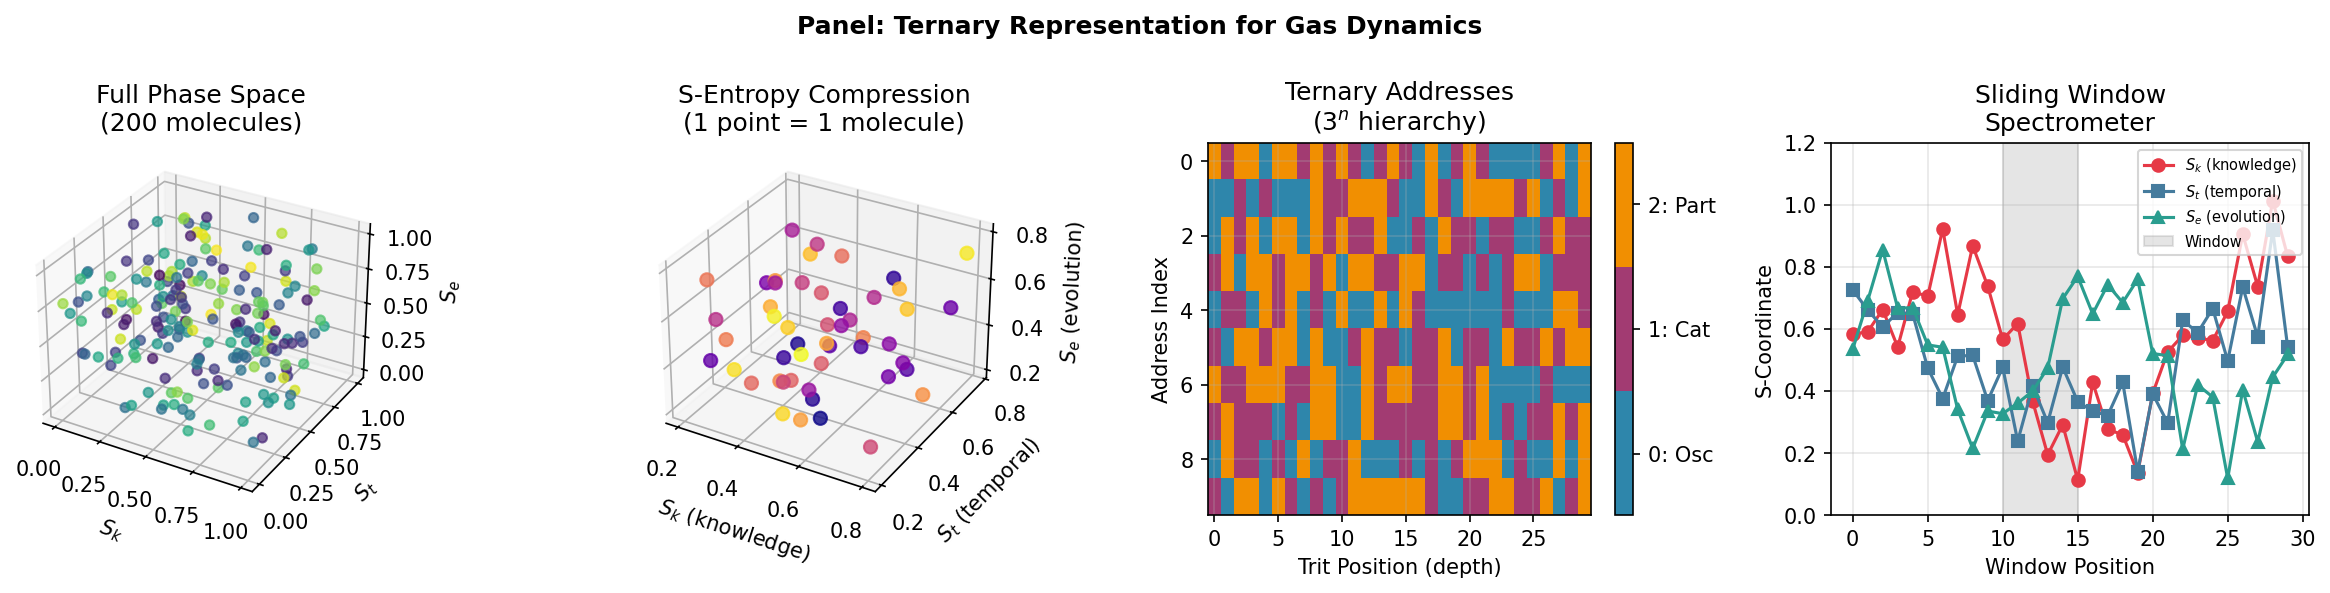
\includegraphics[width=0.95\textwidth]{figures/panel_ternary_computation_1.png}
\caption{\textbf{Ternary Representation for Gas Dynamics: S-Entropy Compression.} Gas dynamics can be represented using ternary (base-3) encoding in S-entropy coordinates, achieving exponential compression of phase space. \textbf{Panel A (Full Phase Space):} 3D scatter plot of 200 virtual gas molecules in categorical S-space $(S_k, S_t, S_e)$, where coordinates are bounded $\in [0,1]^3$. Each point represents a complete molecular state derived from hardware oscillator timing. \textbf{Panel B (S-Entropy Compression):} Compressed representation where each point encodes one molecule's complete state. The mapping from 6D phase space $(x, y, z, v_x, v_y, v_z)$ to 3D S-space achieves $2:1$ dimensional compression while preserving thermodynamic information. \textbf{Panel C (Ternary Addresses):} Heatmap of ternary address encoding showing $3^n$ hierarchical structure. Each row represents one molecule's address; columns show trit positions (depth). Color coding: 0 = Oscillatory (blue), 1 = Categorical (purple), 2 = Partition (orange). \textbf{Panel D (Sliding Window Spectrometer):} Time evolution of S-coordinates as the measurement window slides through the ensemble. The three coordinates $(S_k, S_t, S_e)$ evolve semi-independently, with shaded region indicating the current window position. This demonstrates real-time S-entropy sampling.}
\label{fig:ternary_computation_1}
\end{figure*}

\subsection{Implications for Gas Laws}

The ternary representation framework strengthens the gas law reformulation:

\begin{enumerate}
\item \textbf{Phase space structure:} The $3^k$ hierarchy IS the natural discretization of phase space $\mathcal{S} = [0,1]^3$

\item \textbf{Entropy counting:} The information content of a $k$-trit string is:
\begin{equation}
S = k_B \ln(3^k) = k_B k \ln 3
\end{equation}
This matches the categorical entropy for $M = k$ categories with $n = 3$ states each.

\item \textbf{Temperature:} The rate of trit generation corresponds to $dM/dt$ (Equation~\ref{eq:categorical_temperature}):
\begin{equation}
T = \frac{\hbar}{k_B} \frac{dk}{dt}
\end{equation}

\item \textbf{Pressure:} Trit density in address space corresponds to $\partial M/\partial V$:
\begin{equation}
P = k_B T \left(\frac{\partial k}{\partial V}\right)_{T,N}
\end{equation}
\end{enumerate}

The triple equivalence is not merely conceptual but computational: every ternary operation implements the equivalence between oscillatory, categorical, and partition perspectives.

\subsection{Summary: Ternary as Triple Equivalence}

Ternary representation is the natural encoding of the triple equivalence:

\begin{table}[h]
\centering
\begin{tabular}{p{5cm}p{7cm}}
\hline
\textbf{Ternary Structure} & \textbf{Physical Interpretation} \\
\hline
Three trit values $\{0, 1, 2\}$ & Three perspectives (oscillatory, categorical, partition) \\[0.2cm]
$3^k$ hierarchy & $3^k$ phase space cells in S-entropy space \\[0.2cm]
Trajectory = Address & Path through phase space = Position in phase space \\[0.2cm]
Continuous emergence & Discrete-continuous bridge (categories $\leftrightarrow$ oscillations) \\[0.2cm]
Trit operations & Direct manipulation of three-dimensional structure \\
\hline
\end{tabular}
\caption{Correspondence between ternary structure and physical interpretation.}
\label{tab:ternary_summary}
\end{table}

\textbf{Fundamental insight:} The choice of number base is not merely notational but structural. Binary constrains computation to one-dimensional primitives; ternary provides three-dimensional primitives matching the dimensionality of S-entropy space.

The gas laws, derived from bounded oscillatory dynamics in three-dimensional phase space, find their natural computational form in ternary representation. The triple equivalence---oscillation $\equiv$ category $\equiv$ partition---is encoded in the structure of ternary arithmetic itself.

This suggests a broader principle: \textit{The mathematical structure of physical laws should match the computational structure used to represent them.} Ternary representation is not merely convenient for the triple equivalence framework---it is the native language in which the framework expresses itself.


%=============================================================================
% DISCUSSION AND CONCLUSION
%=============================================================================

\section{Discussion}
\label{sec:discussion}

\subsection{Resolution of Classical Paradoxes}

The triple equivalence framework resolves several long-standing conceptual difficulties in statistical mechanics.

\subsubsection{Resolution-Dependence of Temperature}

Classical kinetic theory defines temperature through the mean square velocity: $T = m\langle v^2\rangle/(3k_B)$. This definition makes temperature dependent on how velocity is measured---the resolution and averaging procedure introduce apparent ambiguity. In the categorical framework, temperature is instead the rate of categorical actualization:
\begin{equation}
T = \frac{\hbar}{k_B}\frac{dM}{dt}
\end{equation}

Categories are discrete and countable; no resolution ambiguity arises. The classical definition emerges as a projection onto the velocity observable, which introduces apparent resolution-dependence through the measurement process. The categorical rate $dM/dt$ is intrinsic to the system and independent of how we choose to observe it.

\subsubsection{Localization of Pressure}

Classical kinetic theory derives pressure from molecular collisions with container walls, suggesting pressure is fundamentally a boundary phenomenon. Yet we routinely measure pressure in the bulk of fluids, far from any boundaries. In the categorical framework, pressure is categorical density:
\begin{equation}
P = k_B T \left(\frac{\partial M}{\partial V}\right)_S
\end{equation}

This is an intrinsic property existing throughout the volume, not localized at boundaries. Wall collisions are one manifestation of categorical density---the rate at which trajectories encounter boundaries---but not its definition. Pressure exists in the bulk because categorical structure exists in the bulk.

\subsubsection{Infinite Velocity Tail}

The Maxwell-Boltzmann distribution $f(v) \propto v^2 e^{-mv^2/(2k_BT)}$ extends to $v \to \infty$, assigning non-zero probability to arbitrarily high velocities. In the categorical framework, the distribution is over discrete categories $m = 0, 1, \ldots, M_{\max}$, where $M_{\max}$ corresponds to $v_{\max} = c$. The distribution is intrinsically bounded:
\begin{equation}
f(m) = \frac{e^{-\beta E_m}}{\sum_{m=0}^{M_{\max}} e^{-\beta E_m}}
\end{equation}

No particle can occupy category $m > M_{\max}$, automatically enforcing $v \leq c$.

\subsection{Unification of Thermodynamics and Computing}

The central insight of this work is that thermodynamics and computation are two perspectives on the same underlying categorical structure. The ideal gas law $PV = Nk_BT$ is simultaneously:
\begin{itemize}
    \item A thermodynamic relation between macroscopic observables
    \item A categorical balance condition in bounded phase space
    \item A constraint on valid solution trajectories in Poincar\'e Computing
\end{itemize}

The processor-oscillator duality ($R_{\text{compute}} = \omega/(2\pi)$) establishes that every oscillator is simultaneously a processor, and vice versa. Hardware timing jitter is not noise to be minimized but categorical information to be exploited.

\subsection{The $\epsilon$-Boundary and Asymptotic Solutions}

Solutions in Poincar\'e Computing are recognized at the $\epsilon$-boundary---exactly one categorical step from closure. This is not approximation but the fundamental nature of categorical computation: categorical irreversibility forbids exact return to the initial state. The ``solution'' IS being one step away; this represents the maximum possible knowledge given G\"odelian constraints.

\section{Conclusion}
\label{sec:conclusion}

We have established that oscillation, categorical distinction, and partition operation are three equivalent descriptions of bounded dynamical systems. From this triple equivalence, we derived:

\textbf{Thermodynamic Results:}
\begin{enumerate}
    \item Entropy in three equivalent forms: $S_{\text{cat}} = k_B M \ln n$, $S_{\text{osc}} = k_B \sum_i \ln(A_i/A_0)$, $S_{\text{part}} = k_B \sum_a \ln(1/s_a)$
    \item Temperature as categorical rate: $T = \hbar(dM/dt)/k_B$
    \item Pressure as categorical density: $P = k_BT(\partial M/\partial V)_S$
    \item The ideal gas law as categorical balance: $PV = Nk_BT$
    \item Maxwell-Boltzmann distribution bounded at $v = c$
\end{enumerate}

\textbf{Computational Results:}
\begin{enumerate}
    \item S-entropy space $\Sspace = [0,1]^3$ satisfies Poincar\'e recurrence
    \item Solutions correspond to recurrent trajectories satisfying constraints
    \item Identity unification: address = processor state = semantic content
    \item Categorical incomparability with Turing computation
    \item Complexity measured in Poincar\'es (categorical completions)
    \item Non-halting dynamics with emergent memory
    \item $3^k$ recursive self-similarity with scale ambiguity
    \item Processor-oscillator duality and processor-memory unification
    \item $\epsilon$-boundary solution recognition
\end{enumerate}

The deeper implication is that thermodynamics and computation are unified through categorical structure in bounded phase space. Temperature measures categorical rate; entropy counts categories; pressure is categorical density; computation is trajectory completion. These are not separate phenomena but projections of a single mathematical structure onto different observables.

All results derive from a single foundational premise: physical systems occupy finite domains. From this boundedness, the triple equivalence structure emerges necessarily, and from the triple equivalence, both statistical mechanics and Poincar\'e Computing follow as mathematical consequences.

\bibliographystyle{plainnat}
\bibliography{references}

\end{document}
